% ==========================================
% BAB IV IMPLEMENTASI
% ==========================================
\cleardoublepage
\chapter{IMPLEMENTASI}
\label{chap:IV}

Bab ini menerapkan DERA pada Kemhan RI menggunakan TOGAF ADM, dari Fase \textit{Preliminary} hingga Fase \textit{Migration Planning}.

\section{Konteks dan Ruang Lingkup Penerapan}
\label{sec:IV.1}

Bab ini merupakan tahap \textit{demonstration} pada DSRM, yaitu penggunaan artefak untuk menyelesaikan satu kasus masalah. Artefak yang didemonstrasikan adalah DERA, sedangkan kasusnya adalah penyusunan EA Kemhan RI sebagai arsitektur turunan. Demonstrasi ini menunjukkan bahwa DERA dapat diterapkan melalui ADM baku (KR-10) dan menghasilkan arsitektur organisasi yang memuat kebutuhan pertahanan, yaitu KR-01 serta KR-03 hingga KR-06 (Tabel~\ref{tab:III.2}).

Kemhan RI dipilih sebagai kasus karena dua alasan. Pertama, Kemhan RI menetapkan kebijakan penyelenggaraan pertahanan negara \cite{UU3Tahun2002}, sehingga berkedudukan sebagai calon pemilik DERA sekaligus pengguna pertamanya. Kedua, tantangan transformasi digital Kemhan RI mencakup seluruh lapisan, mulai dari tata kelola yang belum mengorkestrasi transformasi lintas satuan kerja hingga pusat data tunggal tanpa pusat pemulihan bencana (Tabel~\ref{tab:II.1}). Kondisi tersebut membuat hampir seluruh komponen DERA perlu digunakan. Ruang lingkup penerapan ditetapkan sebagai berikut.

\begin{enumerate}[label=\arabic*.]
\item Organisasi. Arsitektur yang disusun adalah EA Kemhan RI. Mabes TNI, ketiga matra, dan industri pertahanan dicakup pada antarmuka interoperabilitasnya dengan Kemhan RI.
\item Fase ADM. Penerapan dilakukan dari Fase \textit{Preliminary} hingga Fase \textit{Migration Planning}. Fase \textit{Implementation Governance} dan \textit{Architecture Change Management} tidak dilaksanakan, tetapi mekanismenya telah disiapkan pada III.5.3 dan III.5.4.
\item Muatan C6ISR. Lapis operasional C6ISR dimodelkan secara konseptual pada tingkat kapabilitas, antarmuka, dan pola, berdasarkan doktrin, kebijakan, dan sumber terbuka.
\item Horizon waktu. Arsitektur target dan rencana migrasi disusun untuk periode 2026–2030.
\item Sumber data. Data diperoleh dari dokumen dan regulasi Kemhan RI, data portofolio aplikasi dan infrastruktur, serta wawancara dengan unit kerja Kemhan RI.
\end{enumerate}

Penerapan mengikuti panduan pada Tabel~\ref{tab:III.22}. Struktur penerapan pada bab ini disajikan pada Tabel~\ref{tab:IV.1}.

\begingroup\small\setstretch{1.0}
\begin{longtable}{@{}>{\raggedright\arraybackslash\hspace{0pt}}p{0.229\linewidth}>{\raggedright\arraybackslash\hspace{0pt}}p{0.252\linewidth}>{\raggedright\arraybackslash\hspace{0pt}}p{0.312\linewidth}>{\raggedright\arraybackslash\hspace{0pt}}p{0.114\linewidth}@{}}
\caption{Struktur Penerapan DERA pada Kemhan RI}\label{tab:IV.1}\\
\toprule
\textbf{Fase ADM} & \textbf{Komponen DERA} & \textbf{Keluaran Utama} & \textbf{Subbab}\\
\midrule
\endfirsthead
\multicolumn{4}{@{}l}{\small\itshape \tablename\ \thetable{} (lanjutan)}\\
\toprule
\textbf{Fase ADM} & \textbf{Komponen DERA} & \textbf{Keluaran Utama} & \textbf{Subbab}\\
\midrule
\endhead
\bottomrule
\endlastfoot
\textit{Preliminary} & Prinsip, kosakata, \textit{metamodel}, dan tata kelola arsitektur & Prinsip, ruang lingkup, pemangku kepentingan, tata kelola, dan repositori arsitektur & \centering\arraybackslash IV.2\\*
A. \textit{Architecture Vision} & Tujuan strategis, CRM, dan KR & Visi arsitektur, penilaian kapabilitas, dan \textit{Statement of Architecture Work} & \centering\arraybackslash IV.3\\
B. \textit{Business Architecture} & BRA dan CRM & Aliran nilai, peta kapabilitas, dan arsitektur bisnis target & \centering\arraybackslash IV.4\\
C. \textit{Information Systems Architectures} & DRA dan ARA & Arsitektur data dan aplikasi target & \centering\arraybackslash IV.5\\
D. \textit{Technology Architecture} & TRA, posisi teknis, dan pola P3–P5 & Arsitektur teknologi dan keamanan target & \centering\arraybackslash IV.6\\
E. \textit{Opportunities and Solutions} & Pola lintas domain dan ABB & Paket pekerjaan, SBB, arsitektur transisi, dan \textit{roadmap} & \centering\arraybackslash IV.7\\*
F. \textit{Migration Planning} & CRM dan tahapan adopsi & Prioritas paket pekerjaan dan rencana migrasi 2026–2030 & \centering\arraybackslash IV.8\\
\end{longtable}
\endgroup

Tabel~\ref{tab:IV.1} menunjukkan bahwa setiap fase menggunakan komponen DERA sebagai titik awal, kemudian menyesuaikannya dengan kondisi Kemhan RI.

\section{Fase Preliminary}
\label{sec:IV.2}

Fase \textit{Preliminary} menetapkan DERA sebagai acuan EA Kemhan RI dan menyiapkan kapabilitas arsitektur yang dibutuhkan pada fase berikutnya. Fase ini menghasilkan lima keluaran, yaitu prinsip, ruang lingkup, pemangku kepentingan, tata kelola, dan repositori arsitektur.

\subsection{Adopsi Prinsip Arsitektur DERA}
\label{sec:IV.2.1}

Kemhan RI mengadopsi kesembilan prinsip DERA secara utuh karena prinsip termasuk komponen wajib (Tabel~\ref{tab:III.23}). Setiap prinsip kemudian dijabarkan sesuai kondisi Kemhan RI, sebagaimana disajikan pada Tabel~\ref{tab:IV.2}.

\begingroup\small\setstretch{1.0}
\begin{longtable}{@{}>{\raggedright\arraybackslash\hspace{0pt}}p{0.236\linewidth}>{\raggedright\arraybackslash\hspace{0pt}}p{0.489\linewidth}>{\raggedright\arraybackslash\hspace{0pt}}p{0.213\linewidth}@{}}
\caption{Penjabaran Prinsip DERA pada Kemhan RI}\label{tab:IV.2}\\
\toprule
\textbf{Prinsip DERA} & \textbf{Penjabaran pada Kemhan RI} & \textbf{Fase Utama}\\
\midrule
\endfirsthead
\multicolumn{3}{@{}l}{\small\itshape \tablename\ \thetable{} (lanjutan)}\\
\toprule
\textbf{Prinsip DERA} & \textbf{Penjabaran pada Kemhan RI} & \textbf{Fase Utama}\\
\midrule
\endhead
\bottomrule
\endlastfoot
1. \textit{Interoperability} & Pertukaran data antara Kemhan RI, Mabes TNI, matra, dan industri pertahanan dilakukan melalui layanan integrasi dan kamus data bersama. & C dan E\\*
2. \textit{Security by Design} & Setiap aplikasi khusus dan infrastruktur Kemhan RI memiliki klasifikasi sesuai Permenhan Nomor 1 Tahun 2023 dan kendali keamanan sejak perancangan \cite{Permenhan1Tahun2023}. & Seluruh fase, terutama D\\
3. \textit{Data as Strategic Asset} & Data aplikasi khusus dikelola sesuai kebijakan Satu Data Pertahanan, dengan walidata dan kamus data yang ditetapkan. & C\\
4. \textit{Integrated Command \& Control} & Kemhan RI menyediakan kebijakan, data, dan layanan yang mendukung gambaran situasi bersama dengan Mabes TNI, tanpa memodelkan prosedur operasi. & B dan C\\
5. \textit{Availability \& Reliability} & Pusat data Kemhan RI dilengkapi pusat pemulihan bencana untuk menghilangkan titik tunggal kegagalan. & D dan E\\
6. \textit{Scalability \& Flexibility} & Layanan baru dibangun secara modular di atas platform bersama. & D dan E\\
7. \textit{Governance \& Compliance} & Arsitektur Kemhan RI dikelola oleh \textit{Architecture Board} dan diselaraskan dengan Arsitektur SPBE \cite{Perpres132Tahun2022}. & Seluruh fase\\
8. \textit{Smart Defence Oriented} & Setiap inisiatif digital ditelusuri ke sasaran strategis pertahanan sebelum diprioritaskan. & A dan F\\*
9. \textit{User-Centric Service} & Personel Kemhan RI mengakses layanan melalui identitas tunggal dan layanan bersama. & C\\
\end{longtable}
\endgroup

Tabel~\ref{tab:IV.2} menunjukkan bahwa prinsip DERA tidak diubah, tetapi dijabarkan ke dalam kondisi dan permasalahan Kemhan RI. Selain prinsip, Kemhan RI juga mengadopsi kosakata dan \textit{metamodel} DERA, serta menggunakan ArchiMate sebagai notasi pemodelan sesuai posisi teknis DERA \cite{ArchiMate2019}.

\subsection{Ruang Lingkup}
\label{sec:IV.2.2}

Ruang lingkup arsitektur ditetapkan dalam tiga dimensi, yaitu organisasi yang terlibat, unit organisasi Kemhan RI, dan domain arsitektur, sebagaimana ditunjukkan pada Gambar~\ref{fig:IV.1}.

\begin{figure}[htbp]
\centering
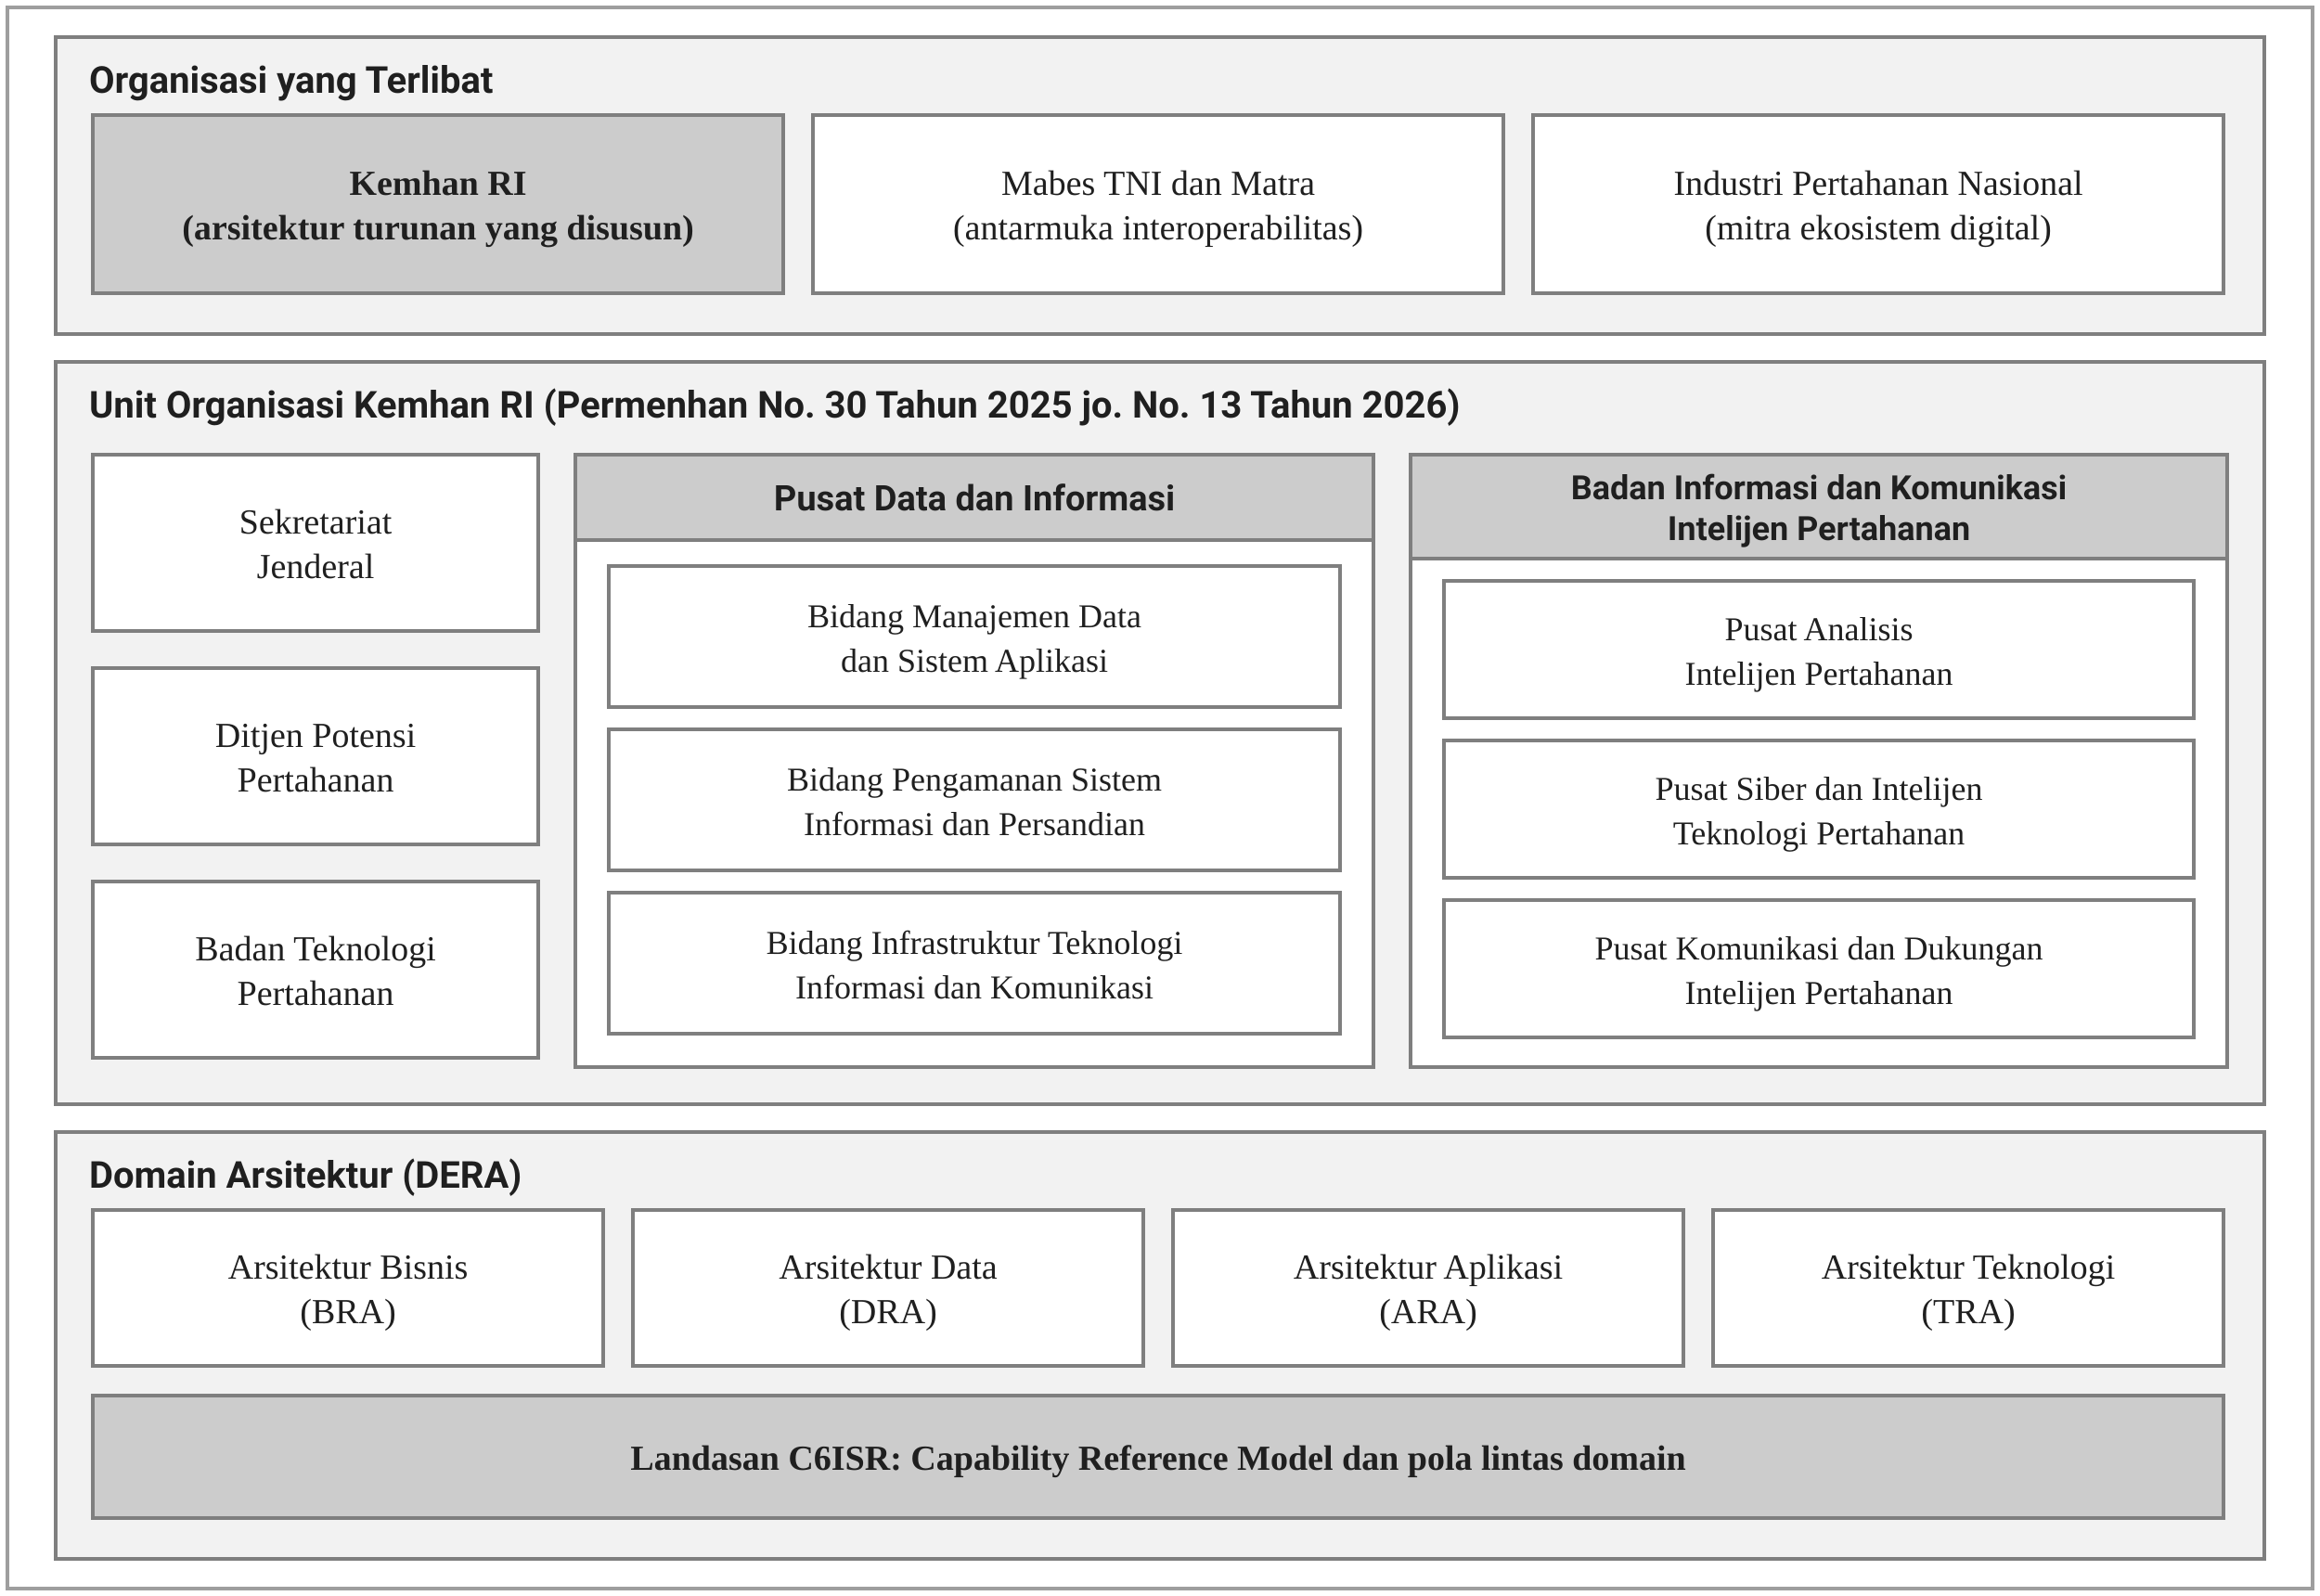
\includegraphics[width=1.00\linewidth,height=0.8\textheight,keepaspectratio]{images/Ruang Lingkup Arsitektur.png}
\caption{Ruang Lingkup Arsitektur}
\label{fig:IV.1}
\end{figure}

Gambar~\ref{fig:IV.1} menunjukkan bahwa Kemhan RI menjadi organisasi inti, Mabes TNI dan ketiga matra terhubung melalui antarmuka interoperabilitas, sedangkan industri pertahanan nasional menjadi mitra ekosistem digital. Dari sisi unit, ruang lingkup mengacu pada Permenhan Nomor 30 Tahun 2025 \cite{Permenhan30Tahun2025} sebagaimana telah diubah dengan Permenhan Nomor 13 Tahun 2026 \cite{Permenhan13Tahun2026}. Pusat Data dan Informasi menyelenggarakan data, sistem informasi, dan infrastruktur TIK, sedangkan fungsi siber dan intelijen teknologi berada pada Badan Informasi dan Komunikasi Intelijen Pertahanan. Dari sisi domain, EA Kemhan RI mencakup keempat domain DERA, dengan C6ISR sebagai landasan melalui CRM dan pola lintas domain.

Lapis CRM disesuaikan dengan mandat Kemhan RI melalui mekanisme seleksi pada III.5.3. Hasil penyesuaian disajikan pada Tabel~\ref{tab:IV.3}.

\begingroup\small\setstretch{1.0}
\begin{longtable}{@{}>{\raggedright\arraybackslash\hspace{0pt}}p{0.248\linewidth}>{\raggedright\arraybackslash\hspace{0pt}}p{0.213\linewidth}>{\raggedright\arraybackslash\hspace{0pt}}p{0.477\linewidth}@{}}
\caption{Penyesuaian Lapis CRM terhadap Mandat Kemhan RI}\label{tab:IV.3}\\
\toprule
\textbf{Lapis CRM} & \textbf{Cakupan} & \textbf{Dasar Penyesuaian}\\
\midrule
\endfirsthead
\multicolumn{3}{@{}l}{\small\itshape \tablename\ \thetable{} (lanjutan)}\\
\toprule
\textbf{Lapis CRM} & \textbf{Cakupan} & \textbf{Dasar Penyesuaian}\\
\midrule
\endhead
\bottomrule
\endlastfoot
Strategis dan tata kelola & Penuh & Kemhan RI menetapkan kebijakan penyelenggaraan pertahanan negara \cite{UU3Tahun2002}.\\*
Operasional C6ISR & Terbatas & Kemhan RI hanya menyediakan kebijakan, standar, data, dan antarmuka dengan Mabes TNI dan matra, karena komando dan pengendalian operasional berada pada Mabes TNI.\\
Pengelolaan sumber daya pertahanan & Penuh & Kemhan RI mengelola personel, anggaran, materiil, dan pengadaan pertahanan \cite{Permenhan30Tahun2025}.\\
Bersama & Penuh & Pusat Data dan Informasi menyelenggarakan data, sistem informasi, dan infrastruktur TIK \cite{Permenhan30Tahun2025,Permenhan13Tahun2026}.\\*
Pendukung & Penuh & Kemhan RI menyelenggarakan telekomunikasi khusus \cite{Permenhan8Tahun2016} dan fungsi siber melalui Badan Informasi dan Komunikasi Intelijen Pertahanan \cite{Permenhan30Tahun2025,Permenhan13Tahun2026}.\\
\end{longtable}
\endgroup

Tabel~\ref{tab:IV.3} menunjukkan bahwa empat lapis dicakup secara penuh, sedangkan lapis operasional C6ISR dicakup secara terbatas. Penyesuaian ini sesuai dengan ruang lingkup penelitian pada I.5 dan tetap menjaga keterpaduan C6ISR melalui antarmuka dengan Mabes TNI dan matra.

\subsection{Identifikasi Stakeholder}
\label{sec:IV.2.3}

Identifikasi pemangku kepentingan dilakukan untuk mengenali pihak yang memengaruhi atau dipengaruhi arsitektur, beserta \textit{concern}, tingkat pengaruh, dan kebutuhan utamanya. Hasilnya disajikan pada Tabel~\ref{tab:IV.4}.

\begingroup\small\setstretch{1.0}
\begin{longtable}{@{}>{\raggedright\arraybackslash\hspace{0pt}}p{0.072\linewidth}>{\raggedright\arraybackslash\hspace{0pt}}p{0.215\linewidth}>{\raggedright\arraybackslash\hspace{0pt}}p{0.232\linewidth}>{\raggedright\arraybackslash\hspace{0pt}}p{0.121\linewidth}>{\raggedright\arraybackslash\hspace{0pt}}p{0.236\linewidth}@{}}
\caption{Matriks Pemangku Kepentingan}\label{tab:IV.4}\\
\toprule
\textbf{No.} & \textbf{Pemangku Kepentingan} & \textbf{\textit{Concern}} & \textbf{Pengaruh} & \textbf{Kebutuhan Utama}\\
\midrule
\endfirsthead
\multicolumn{5}{@{}l}{\small\itshape \tablename\ \thetable{} (lanjutan)}\\
\toprule
\textbf{No.} & \textbf{Pemangku Kepentingan} & \textbf{\textit{Concern}} & \textbf{Pengaruh} & \textbf{Kebutuhan Utama}\\
\midrule
\endhead
\bottomrule
\endlastfoot
\centering\arraybackslash 1 & Menteri Pertahanan & Arah strategis dan kedaulatan pertahanan & Sangat tinggi & Informasi eksekutif dan keputusan berbasis data\\*
\centering\arraybackslash 2 & Sekretaris Jenderal & Koordinasi dan tata kelola organisasi & Tinggi & Integrasi lintas unit dan kepatuhan SPBE\\
\centering\arraybackslash 3 & Kepala Pusat Data dan Informasi & Pengelolaan data, sistem informasi, dan infrastruktur TIK & Sangat tinggi & Infrastruktur TIK terpadu dan tata kelola data\\
\centering\arraybackslash 4 & Pusat Siber dan Intelijen Teknologi Pertahanan & Keamanan dan intelijen siber pertahanan & Tinggi & Penerapan \textit{security by design} dan pusat operasi keamanan\\
\centering\arraybackslash 5 & Ditjen Potensi Pertahanan & Potensi dan industri pertahanan & Tinggi & Data potensi pertahanan dan kolaborasi industri\\
\centering\arraybackslash 6 & Ditjen Strategi Pertahanan dan Ditjen Perencanaan Pertahanan & Perumusan strategi dan perencanaan & Tinggi & Data perencanaan pertahanan yang terintegrasi\\
\centering\arraybackslash 7 & Mabes TNI dan matra (TNI AD\label{sk:AD}, AL\label{sk:AL}, dan AU\label{sk:AU}) & Operasi dan interoperabilitas lintas matra & Tinggi & Pertukaran data dan dukungan komando-kendali\\
\centering\arraybackslash 8 & Badan Teknologi Pertahanan & Pengembangan teknologi pertahanan & Sedang & Standar teknologi dan dukungan inovasi\\
\centering\arraybackslash 9 & Industri pertahanan nasional & Kolaborasi dan alih teknologi & Sedang & Standar terbuka dan interoperabilitas\\*
\centering\arraybackslash 10 & Personel dan pengguna layanan & Kemudahan dan keandalan layanan & Sedang & Layanan digital yang berorientasi pengguna\\
\end{longtable}
\endgroup

Tabel~\ref{tab:IV.4} menunjukkan bahwa Menteri Pertahanan dan Kepala Pusat Data dan Informasi memiliki pengaruh sangat tinggi, sehingga keduanya menjadi sasaran utama komunikasi arsitektur. Mabes TNI dan matra memiliki pengaruh tinggi karena menjadi pengguna DERA berikutnya dan pihak utama pada antarmuka C6ISR.

\subsection{Governance}
\label{sec:IV.2.4}

Pusat Data dan Informasi telah berkedudukan langsung di bawah Menteri Pertahanan. Namun, mandatnya bersifat pengelolaan operasional (\textit{run-the-engine}) dan belum mencakup orkestrasi transformasi digital lintas satuan kerja dan matra. Oleh karena itu, tata kelola arsitektur menambahkan fungsi \textit{Chief Digital Transformation Officer} (CDTO\label{sk:CDTO}) pada tingkat strategis di bawah Menteri Pertahanan. Karena Kemhan RI juga berkedudukan sebagai pemilik DERA, struktur tata kelola mencakup pengelolaan DERA dan EA Kemhan RI, sebagaimana disajikan pada Tabel~\ref{tab:IV.5}.

\begingroup\small\setstretch{1.0}
\begin{longtable}{@{}>{\raggedright\arraybackslash\hspace{0pt}}p{0.201\linewidth}>{\raggedright\arraybackslash\hspace{0pt}}p{0.382\linewidth}>{\raggedright\arraybackslash\hspace{0pt}}p{0.355\linewidth}@{}}
\caption{Struktur Tata Kelola Arsitektur}\label{tab:IV.5}\\
\toprule
\textbf{Elemen} & \textbf{Penanggung Jawab} & \textbf{Peran Utama}\\
\midrule
\endfirsthead
\multicolumn{3}{@{}l}{\small\itshape \tablename\ \thetable{} (lanjutan)}\\
\toprule
\textbf{Elemen} & \textbf{Penanggung Jawab} & \textbf{Peran Utama}\\
\midrule
\endhead
\bottomrule
\endlastfoot
Pemilik arsitektur & Menteri Pertahanan sebagai pemilik utama, dengan Kepala Pusat Data dan Informasi sebagai pemilik pelaksana & Memiliki, membiayai, dan menjamin keberlanjutan DERA serta EA Kemhan RI, termasuk menetapkan versi baru DERA\\*
\textit{Architecture Board} & Diketuai CDTO, dengan anggota Kepala Pusat Data dan Informasi, Kepala Badan Informasi dan Komunikasi Intelijen Pertahanan, para Direktur Jenderal terkait, serta perwakilan Mabes TNI dan matra; Sekretaris Jenderal sebagai pengarah & Menetapkan prinsip, menyetujui \textit{Request for Architecture Work}, meninjau kesesuaian berdasarkan KK-01 hingga KK-09, memutuskan dispensasi, dan membahas usulan pemutakhiran DERA\\
\textit{Architecture Team} & Dipimpin CDTO, dengan Pusat Data dan Informasi sebagai pelaksana & Menjalankan ADM dengan DERA sebagai acuan dan memelihara repositori arsitektur\\*
Tim keamanan siber & Bidang Pengamanan Sistem Informasi dan Persandian bersama Pusat Siber dan Intelijen Teknologi Pertahanan & Menjamin penerapan \textit{security by design} dan pemisahan domain klasifikasi pada seluruh fase\\
\end{longtable}
\endgroup

Tabel~\ref{tab:IV.5} menunjukkan bahwa CDTO memimpin \textit{Architecture Board} dan \textit{Architecture Team}, sedangkan Pusat Data dan Informasi berperan sebagai pelaksana. Pembagian ini memisahkan fungsi perubahan (\textit{change-the-business}) dari fungsi operasional (\textit{run-the-engine}). Keikutsertaan Mabes TNI dan matra dalam \textit{Architecture Board} menjadikan forum tersebut sebagai dewan arsitektur DERA pada III.5.3.

\subsection{Repositori Arsitektur}
\label{sec:IV.2.5}

Repositori arsitektur Kemhan RI disusun mengikuti kelas \textit{Architecture Repository} TOGAF \cite{TOGAF2022} dan penempatan komponen DERA pada Tabel~\ref{tab:III.21}. Struktur repositori disajikan pada Tabel~\ref{tab:IV.6}.

\begingroup\small\setstretch{1.0}
\begin{longtable}{@{}>{\raggedright\arraybackslash\hspace{0pt}}p{0.354\linewidth}>{\raggedright\arraybackslash\hspace{0pt}}p{0.615\linewidth}@{}}
\caption{Struktur Repositori Arsitektur Kemhan RI}\label{tab:IV.6}\\
\toprule
\textbf{Bagian Repositori} & \textbf{Muatan Utama}\\
\midrule
\endfirsthead
\multicolumn{2}{@{}l}{\small\itshape \tablename\ \thetable{} (lanjutan)}\\
\toprule
\textbf{Bagian Repositori} & \textbf{Muatan Utama}\\
\midrule
\endhead
\bottomrule
\endlastfoot
\textit{Architecture Metamodel} & \textit{Metamodel} dan kosakata DERA, serta notasi ArchiMate\\*
\textit{Reference Library} & DERA versi yang digunakan, serta katalog regulasi SPBE, Satu Data, dan pelindungan infrastruktur informasi vital\\
\textit{Standards Library} & Posisi teknis DERA dan standar teknis internal Kemhan RI\\
\textit{Architecture Requirements Repository} & Kebutuhan arsitektur Kemhan RI yang ditelusuri ke KR DERA\\
\textit{Architecture Landscape} & Arsitektur \textit{baseline}, target, dan transisi Kemhan RI pada domain bisnis, data, aplikasi, dan teknologi\\*
\textit{Governance Repository} & Keputusan \textit{Architecture Board}, hasil tinjauan kesesuaian, dan catatan dispensasi\\
\end{longtable}
\endgroup

Tabel~\ref{tab:IV.6} menunjukkan bahwa DERA disimpan sebagai acuan pada \textit{Reference Library} dan \textit{Standards Library}, sedangkan EA Kemhan RI disimpan pada \textit{Architecture Landscape}. Artefak terkait C6ISR tidak disimpan terpisah, tetapi ditandai dengan lapis CRM dan pola lintas domain, sehingga dapat ditelusuri lintas domain.

\section{Fase A: Architecture Vision}
\label{sec:IV.3}

Fase \textit{Architecture Vision} menetapkan arah EA Kemhan RI dengan tujuan strategis DERA, CRM, dan KR sebagai masukan. Fase ini menghasilkan enam keluaran, yaitu visi dan tujuan, pendorong dan kendala, penilaian kapabilitas, risiko dan mitigasi, konsep solusi, serta \textit{Statement of Architecture Work}.

\subsection{Visi, Misi, dan Tujuan Arsitektur}
\label{sec:IV.3.1}

Visi arsitektur transformasi digital Kemhan RI dirumuskan sebagai berikut.

“Terwujudnya arsitektur transformasi digital pertahanan yang terintegrasi, aman, dan berorientasi pertahanan cerdas untuk mewujudkan keunggulan informasi serta mendukung pengambilan keputusan yang cepat dan tepat di lingkungan Kemhan RI dan TNI.”

Visi tersebut dijabarkan ke dalam lima misi berikut.

\begin{enumerate}[label=\arabic*.]
\item Mewujudkan interoperabilitas dan integrasi data lintas unit Kemhan RI, Mabes TNI, dan ketiga matra.
\item Menerapkan keamanan siber sejak perancangan pada seluruh sistem pertahanan.
\item Menyediakan layanan digital yang andal dan berorientasi pengguna.
\item Menyediakan kebijakan, data, dan layanan yang mendukung keterpaduan C6ISR bersama Mabes TNI dan matra.
\item Menyelenggarakan tata kelola digital yang selaras dengan SPBE dan Satu Data Indonesia.
\end{enumerate}

Visi dan misi tersebut diturunkan menjadi tujuan strategis. Setiap tujuan ditautkan pada prinsip DERA dan lapis CRM, sebagaimana disajikan pada Tabel~\ref{tab:IV.7}.

\begingroup\small\setstretch{1.0}
\begin{longtable}{@{}>{\raggedright\arraybackslash\hspace{0pt}}p{0.069\linewidth}>{\raggedright\arraybackslash\hspace{0pt}}p{0.393\linewidth}>{\raggedright\arraybackslash\hspace{0pt}}p{0.240\linewidth}>{\raggedright\arraybackslash\hspace{0pt}}p{0.206\linewidth}@{}}
\caption{Tujuan Strategis Arsitektur}\label{tab:IV.7}\\
\toprule
\textbf{No.} & \textbf{Tujuan Strategis} & \textbf{Prinsip DERA} & \textbf{Lapis CRM}\\
\midrule
\endfirsthead
\multicolumn{4}{@{}l}{\small\itshape \tablename\ \thetable{} (lanjutan)}\\
\toprule
\textbf{No.} & \textbf{Tujuan Strategis} & \textbf{Prinsip DERA} & \textbf{Lapis CRM}\\
\midrule
\endhead
\bottomrule
\endlastfoot
\centering\arraybackslash 1 & Mewujudkan integrasi data dan sistem antara Kemhan RI, Mabes TNI, dan matra & \textit{Interoperability} & Bersama\\*
\centering\arraybackslash 2 & Memperkuat keamanan siber pertahanan secara menyeluruh & \textit{Security by Design} & Pendukung\\
\centering\arraybackslash 3 & Mengelola data pertahanan sebagai aset strategis pengambilan keputusan & \textit{Data as Strategic Asset} & Bersama\\
\centering\arraybackslash 4 & Menyediakan dukungan C6ISR yang terpadu bersama Mabes TNI & \textit{Integrated Command \& Control} & Operasional C6ISR\\
\centering\arraybackslash 5 & Menjamin ketersediaan layanan pertahanan yang andal & \textit{Availability \& Reliability} & Bersama dan pendukung\\
\centering\arraybackslash 6 & Meningkatkan kualitas layanan dan efektivitas personel & \textit{User-Centric Service} & Pengelolaan sumber daya\\*
\centering\arraybackslash 7 & Menjamin tata kelola dan kepatuhan transformasi digital pertahanan & \textit{Governance \& Compliance}; \textit{Smart Defence Oriented} & Strategis dan tata kelola\\
\end{longtable}
\endgroup

Tabel~\ref{tab:IV.7} menunjukkan bahwa setiap tujuan strategis dapat ditelusuri ke prinsip DERA dan lapis CRM. Prinsip \textit{Scalability \& Flexibility} tidak dijadikan tujuan tersendiri, tetapi diterapkan sebagai kriteria perancangan pada Fase D.

\subsection{Pendorong dan Kendala}
\label{sec:IV.3.2}

Pendorong dan kendala transformasi dirangkum pada Tabel~\ref{tab:IV.8}. Pendorong utama berasal dari arah RPJPN 2025–2045 \cite{UU59Tahun2024}, kebijakan SPBE \cite{Perpres95Tahun2018}, percepatan transformasi digital \cite{Perpres82Tahun2023}, dan Satu Data Indonesia \cite{Perpres39Tahun2019}.

\begingroup\small\setstretch{1.0}
\begin{longtable}{@{}>{\raggedright\arraybackslash\hspace{0pt}}p{0.208\linewidth}>{\raggedright\arraybackslash\hspace{0pt}}p{0.761\linewidth}@{}}
\caption{Pendorong dan Kendala Transformasi Digital Pertahanan}\label{tab:IV.8}\\
\toprule
\textbf{Aspek} & \textbf{Uraian}\\
\midrule
\endfirsthead
\multicolumn{2}{@{}l}{\small\itshape \tablename\ \thetable{} (lanjutan)}\\
\toprule
\textbf{Aspek} & \textbf{Uraian}\\
\midrule
\endhead
\bottomrule
\endlastfoot
Pendorong & Arah modernisasi pertahanan dalam RPJPN 2025–2045; kebijakan SPBE dan Satu Data Indonesia; meningkatnya ancaman siber dan tuntutan operasi multidomain; kebutuhan interoperabilitas lintas matra; serta tuntutan pengambilan keputusan berbasis data.\\
Kendala & Fragmentasi sistem dan data yang tersilo; keterbatasan SDM digital; keberadaan sistem lama (\textit{legacy}); aspek kerahasiaan pertahanan; serta keterbatasan anggaran dan waktu.\\
\end{longtable}
\endgroup

Tabel~\ref{tab:IV.8} menunjukkan bahwa pendorong transformasi bersifat eksternal dan didukung regulasi, sedangkan kendalanya terutama bersifat internal, yaitu kondisi sistem, data, dan SDM.

\subsection{Penilaian Kapabilitas Berbasis Capability Reference Model}
\label{sec:IV.3.3}

Penilaian kapabilitas memetakan kondisi Kemhan RI pada setiap kapabilitas CRM. Setiap kapabilitas dinilai dengan tiga status, yaitu tersedia, parsial, dan belum tersedia. Kapabilitas tersedia berarti fungsi dan dukungan digitalnya telah berjalan, kapabilitas parsial berarti fungsinya ada tetapi dukungan digitalnya terfragmentasi, sedangkan kapabilitas belum tersedia berarti fungsinya belum memiliki penanggung jawab. Hasil penilaian ditunjukkan pada Gambar~\ref{fig:IV.2}.

\begin{figure}[htbp]
\centering
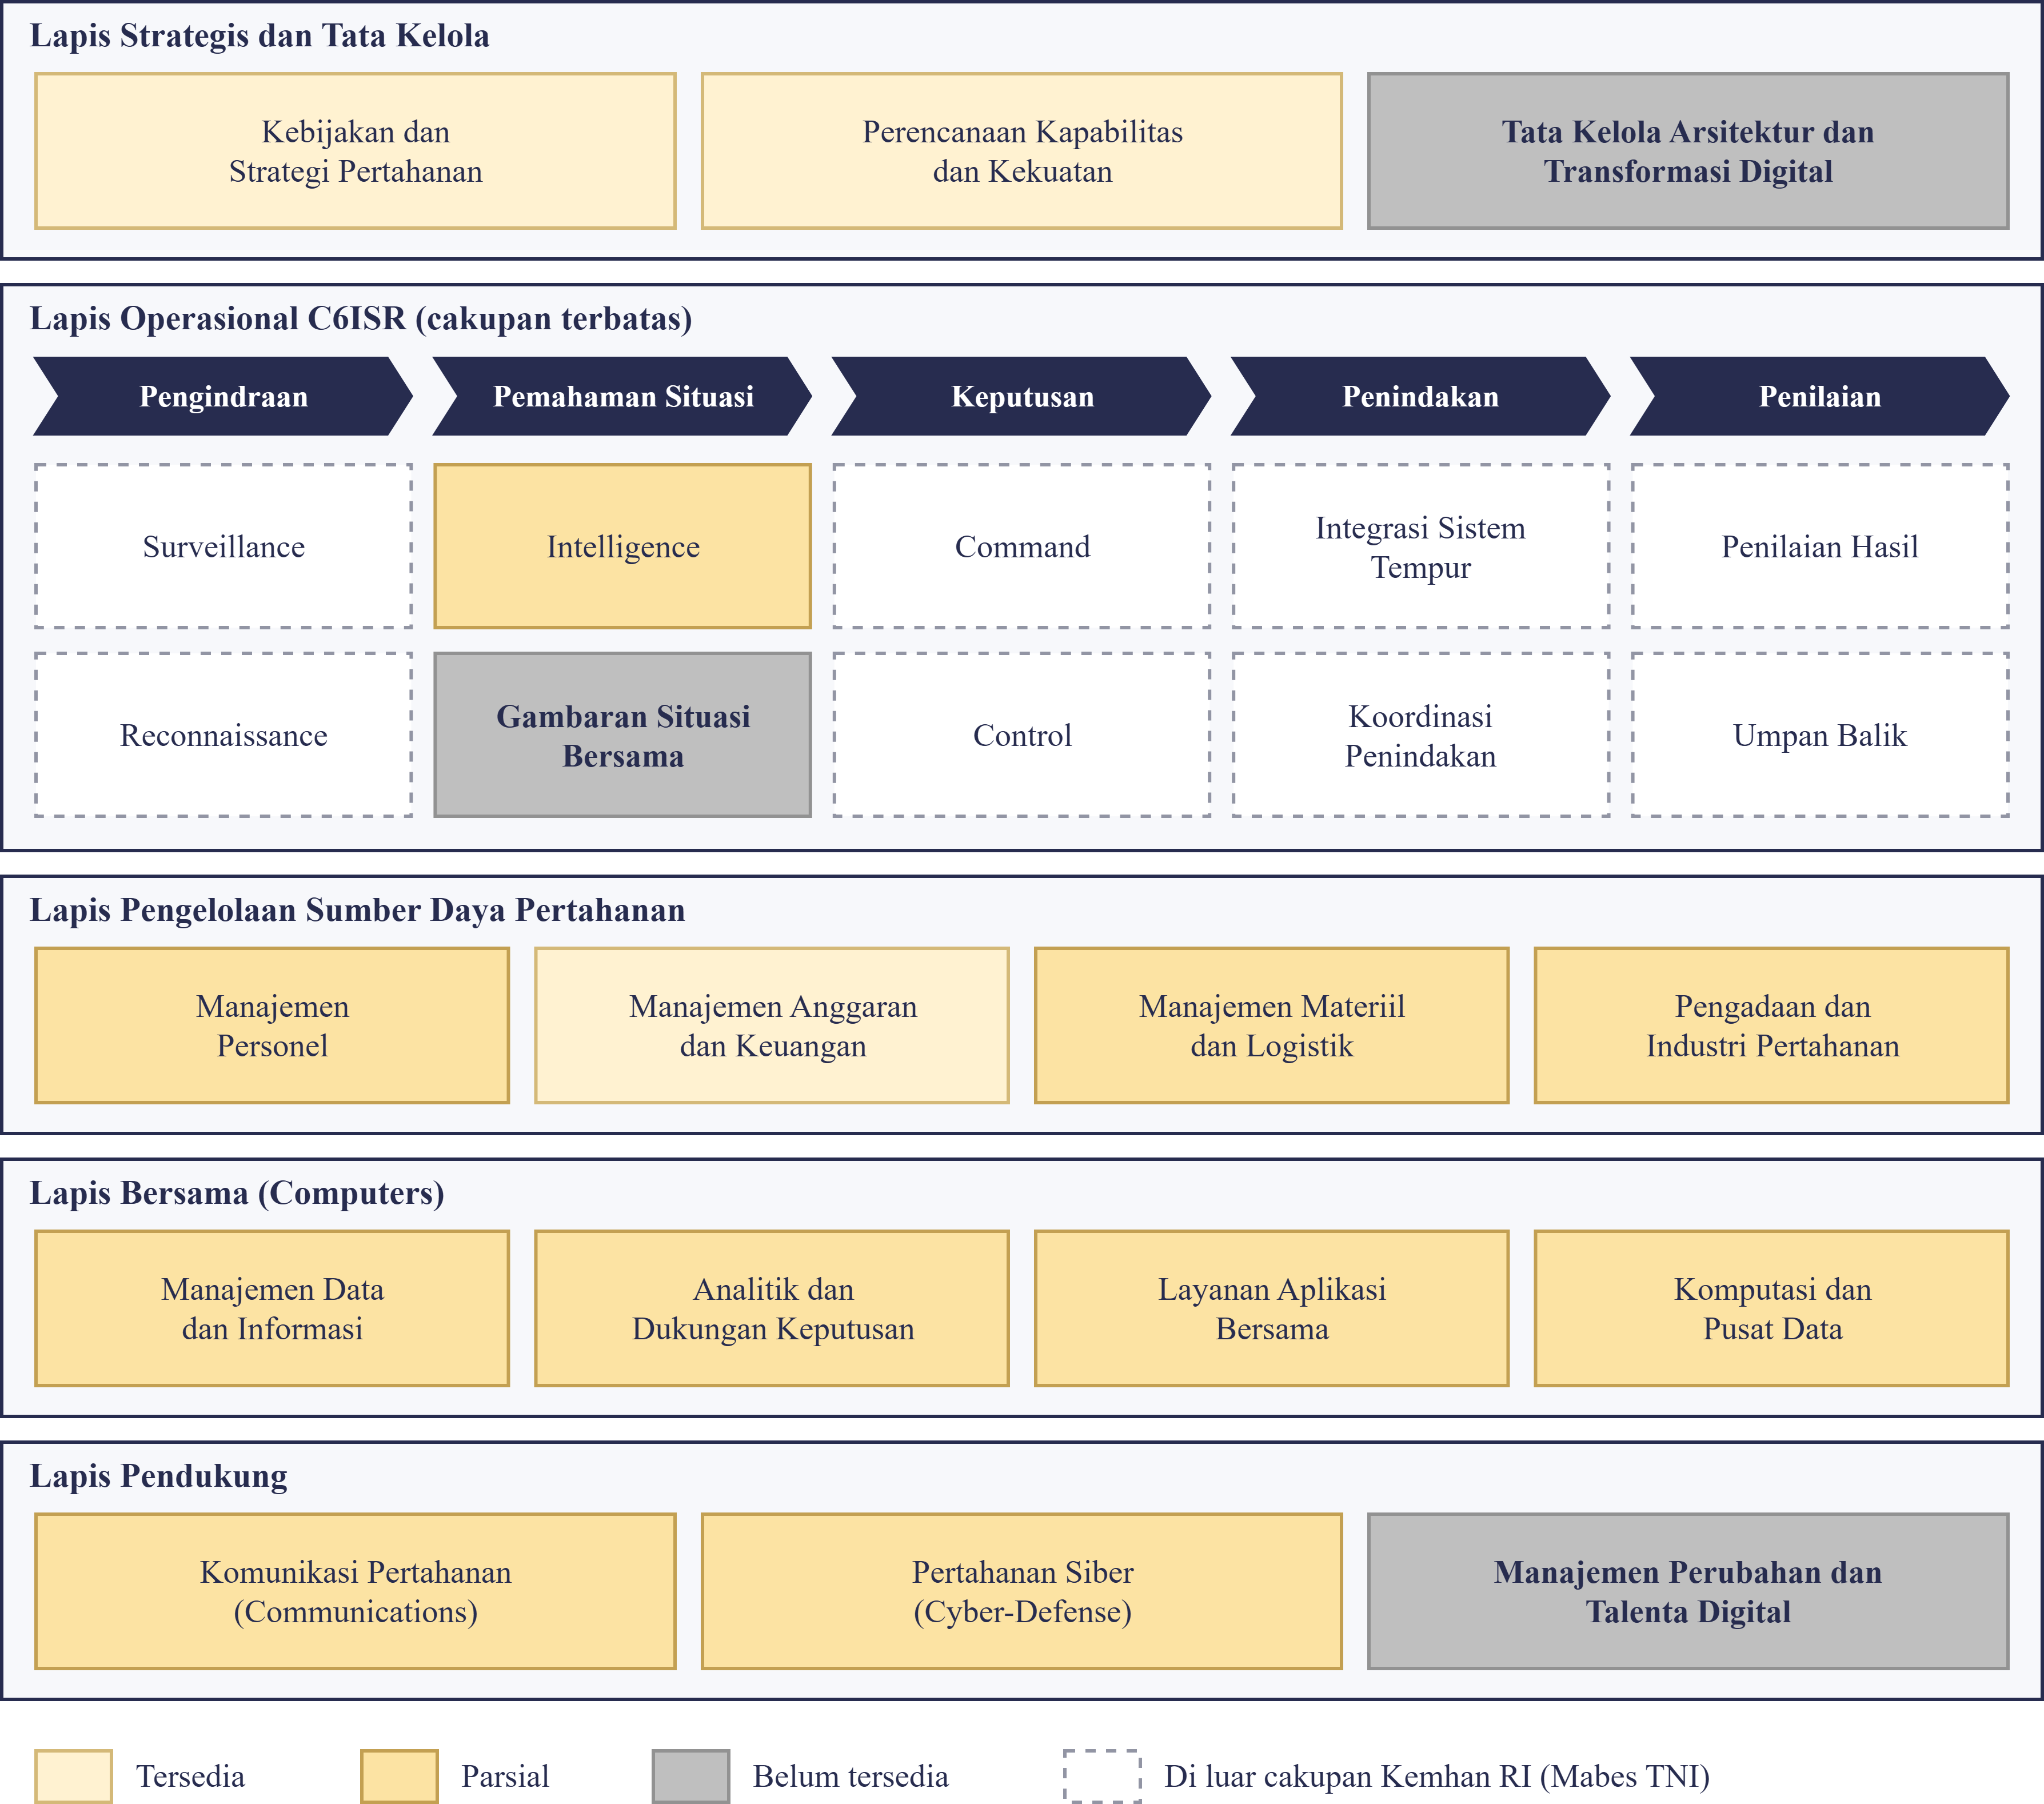
\includegraphics[width=1.00\linewidth,height=0.8\textheight,keepaspectratio]{images/Gambar_IV.2_Penilaian_Kapabilitas_CRM_Berwarna.drawio.png}
\caption{Penilaian Kapabilitas Kemhan RI pada \textit{Capability Reference Model}}
\label{fig:IV.2}
\end{figure}

Gambar~\ref{fig:IV.2} menunjukkan bahwa sebagian besar kapabilitas Kemhan RI berstatus parsial. Dasar penilaian setiap lapis disajikan pada Tabel~\ref{tab:IV.9}.

\begingroup\small\setstretch{1.0}
\begin{longtable}{@{}>{\raggedright\arraybackslash\hspace{0pt}}p{0.189\linewidth}>{\raggedright\arraybackslash\hspace{0pt}}p{0.323\linewidth}>{\raggedright\arraybackslash\hspace{0pt}}p{0.426\linewidth}@{}}
\caption{Dasar Penilaian Kapabilitas per Lapis CRM}\label{tab:IV.9}\\
\toprule
\textbf{Lapis CRM} & \textbf{Status Kapabilitas} & \textbf{Kondisi Saat Ini}\\
\midrule
\endfirsthead
\multicolumn{3}{@{}l}{\small\itshape \tablename\ \thetable{} (lanjutan)}\\
\toprule
\textbf{Lapis CRM} & \textbf{Status Kapabilitas} & \textbf{Kondisi Saat Ini}\\
\midrule
\endhead
\bottomrule
\endlastfoot
Strategis dan tata kelola & Tersedia: kebijakan dan strategi, serta perencanaan kapabilitas dan kekuatan. Belum tersedia: tata kelola arsitektur dan transformasi digital. & Fungsi kebijakan dan perencanaan telah dijalankan direktorat jenderal terkait, tetapi belum ada unit yang mengorkestrasi transformasi digital lintas satuan kerja dan matra (Tabel~\ref{tab:II.1}).\\*
Operasional C6ISR & Parsial: \textit{intelligence}. Belum tersedia: gambaran situasi bersama. & Analisis intelijen pertahanan dijalankan Badan Informasi dan Komunikasi Intelijen Pertahanan, tetapi sistem dengan standar berbeda sulit bertukar informasi, sehingga gambaran situasi bersama dengan Mabes TNI belum tersedia.\\
Pengelolaan sumber daya pertahanan & Tersedia: anggaran dan keuangan. Parsial: personel, materiil dan logistik, serta pengadaan dan industri pertahanan. & Pengelolaan anggaran didukung aplikasi umum SPBE, sedangkan aplikasi khusus untuk personel, logistik, dan potensi pertahanan berjalan terpisah dengan mekanisme autentikasi berbeda.\\
Bersama & Parsial: seluruh kapabilitas. & Data terkotak per aplikasi tanpa kamus data dan klasifikasi, integrasi akses tunggal baru dirintis \cite{Pusdatin2026SSO}, dan seluruh layanan bertumpu pada satu pusat data tanpa pusat pemulihan bencana.\\*
Pendukung & Parsial: komunikasi pertahanan dan pertahanan siber. Belum tersedia: manajemen perubahan dan talenta digital. & Infrastruktur tersedia tetapi belum sepenuhnya terpadu, pengamanan siber masih parsial, dan kompetensi digital belum merata.\\
\end{longtable}
\endgroup

Tabel~\ref{tab:IV.9} menunjukkan bahwa dari 16 kapabilitas dalam cakupan Kemhan RI, tiga kapabilitas tersedia, sepuluh parsial, dan tiga belum tersedia. Kesenjangan terbesar terdapat pada lapis bersama, sejalan dengan empat permasalahan prioritas Satu Data Pertahanan, yaitu kelembagaan dan koordinasi, kualitas data, integrasi sistem, dan kapasitas SDM \cite{Pusdatin2026SatuData}. Tiga kapabilitas yang belum tersedia menjadi prioritas pada Fase B hingga D.

\subsection{Risiko dan Mitigasi}
\label{sec:IV.3.4}

Risiko transformasi diidentifikasi untuk mengantisipasi hambatan dalam mencapai arsitektur target. Setiap risiko disertai tindakan mitigasi, sebagaimana disajikan pada Tabel~\ref{tab:IV.10}.

\begingroup\small\setstretch{1.0}
\begin{longtable}{@{}>{\raggedright\arraybackslash\hspace{0pt}}p{0.069\linewidth}>{\raggedright\arraybackslash\hspace{0pt}}p{0.263\linewidth}>{\raggedright\arraybackslash\hspace{0pt}}p{0.255\linewidth}>{\raggedright\arraybackslash\hspace{0pt}}p{0.320\linewidth}@{}}
\caption{Risiko Transformasi dan Mitigasi}\label{tab:IV.10}\\
\toprule
\textbf{No.} & \textbf{Risiko} & \textbf{Dampak} & \textbf{Mitigasi}\\
\midrule
\endfirsthead
\multicolumn{4}{@{}l}{\small\itshape \tablename\ \thetable{} (lanjutan)}\\
\toprule
\textbf{No.} & \textbf{Risiko} & \textbf{Dampak} & \textbf{Mitigasi}\\
\midrule
\endhead
\bottomrule
\endlastfoot
\centering\arraybackslash 1 & Resistensi perubahan organisasi & Adopsi arsitektur berjalan lambat & Manajemen perubahan, dukungan pimpinan, dan fungsi CDTO\\*
\centering\arraybackslash 2 & Keterbatasan SDM digital & Kualitas implementasi menurun & Pelatihan, rekrutmen, dan kerja sama kelembagaan\\
\centering\arraybackslash 3 & Kompleksitas integrasi sistem \textit{legacy} & Keterlambatan dan pembengkakan biaya & Penerapan bertahap, layanan integrasi dan API\label{sk:API}, serta standar terbuka\\
\centering\arraybackslash 4 & Ancaman siber selama transisi & Kebocoran atau gangguan data & Penerapan \textit{security by design} dan penguatan fungsi keamanan siber\\
\centering\arraybackslash 5 & Ketergantungan pada teknologi asing & Risiko terhadap kedaulatan data & Mengutamakan teknologi dalam negeri dan standar terbuka\\
\centering\arraybackslash 6 & Keterbatasan anggaran dan waktu & Cakupan target tidak tercapai & Prioritas berbasis nilai dan \textit{roadmap} bertahap\\*
\centering\arraybackslash 7 & Penerapan DERA tidak seragam antarorganisasi pertahanan & Interoperabilitas lintas organisasi tidak tercapai & Kriteria kesesuaian KK-01 hingga KK-09 dan tinjauan oleh \textit{Architecture Board} yang melibatkan Mabes TNI dan matra\\
\end{longtable}
\endgroup

Tabel~\ref{tab:IV.10} menunjukkan bahwa sebagian besar risiko bersifat organisasional. Risiko ketujuh muncul karena DERA digunakan bersama, sehingga mitigasinya bertumpu pada tata kelola DERA.

\subsection{Konsep Solusi}
\label{sec:IV.3.5}

Konsep solusi memberikan gambaran menyeluruh mengenai arsitektur target. Konsep ini disusun berlapis dengan mengacu pada pola lintas domain DERA, sebagaimana ditunjukkan pada Gambar~\ref{fig:IV.3}.

\begin{figure}[htbp]
\centering
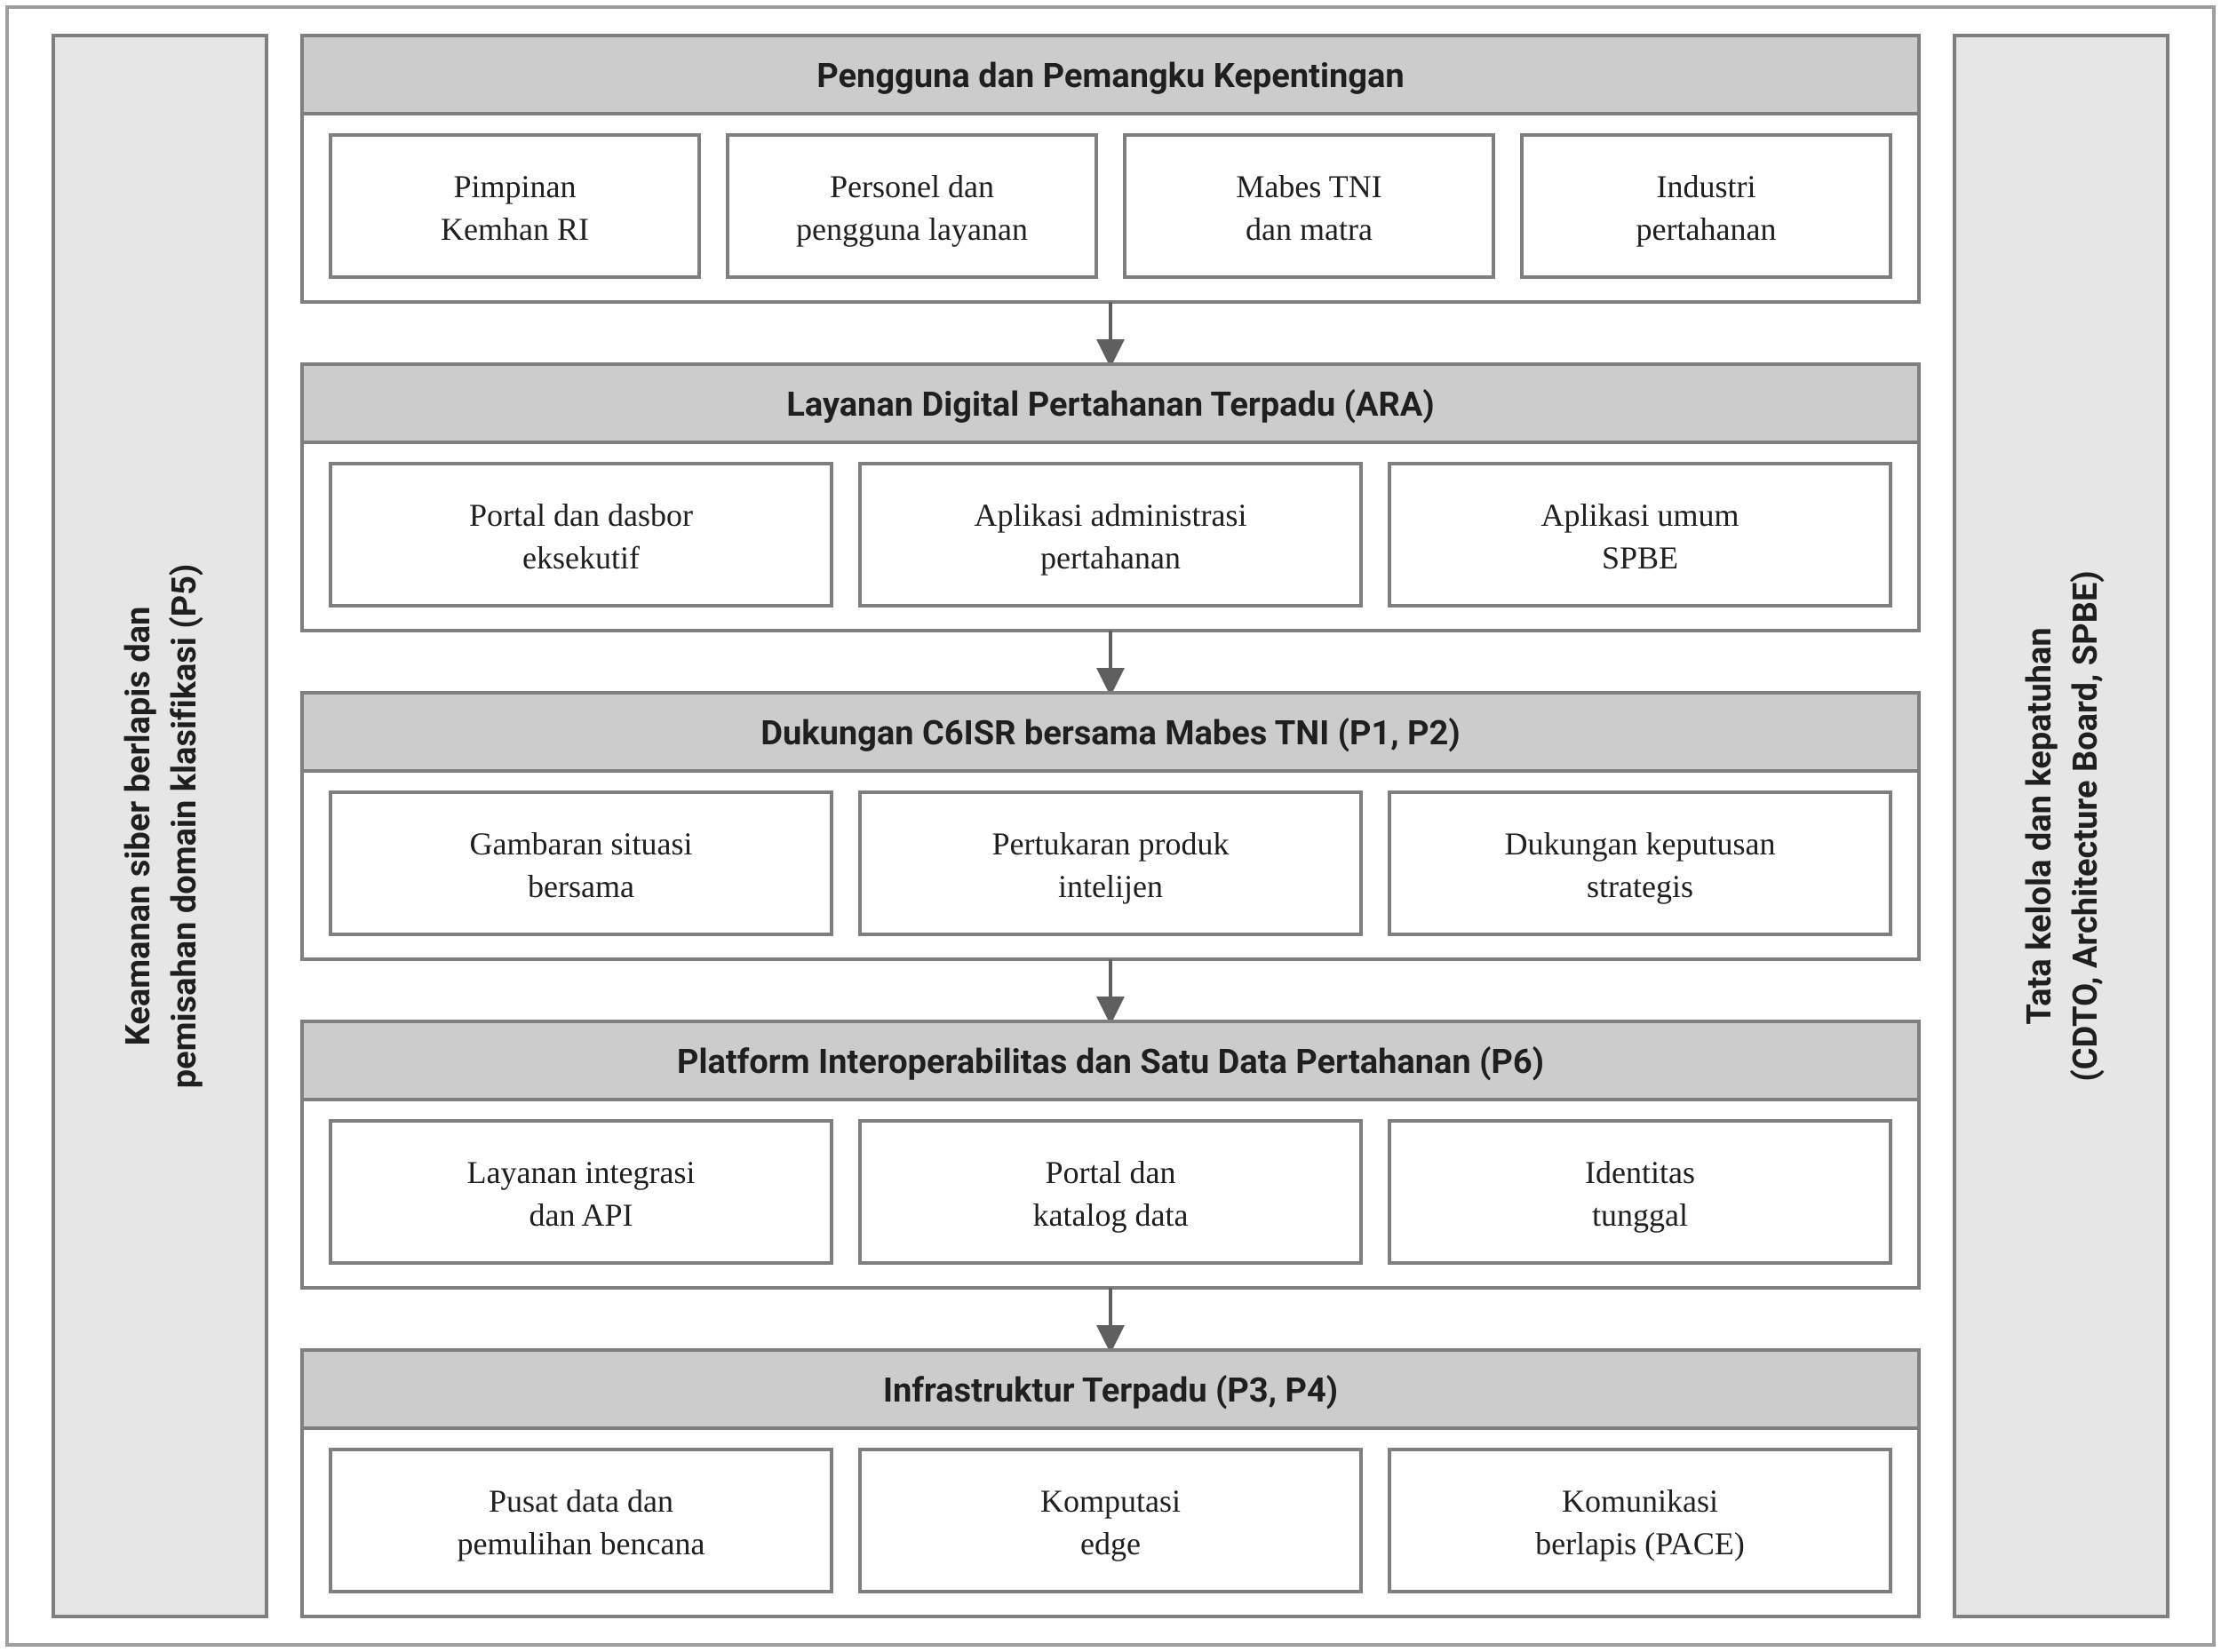
\includegraphics[width=1.00\linewidth,height=0.8\textheight,keepaspectratio]{images/Konsep Solusi Arsitektur Target.png}
\caption{Konsep Solusi Arsitektur Target}
\label{fig:IV.3}
\end{figure}

Gambar~\ref{fig:IV.3} menunjukkan bahwa infrastruktur terpadu menjadi fondasi, platform interoperabilitas dan Satu Data Pertahanan menjadi simpul integrasi, dukungan C6ISR bersama Mabes TNI menjadi muatan khas pertahanan, dan layanan digital menjadi antarmuka bagi pengguna. Keamanan siber serta tata kelola dan kepatuhan membentang pada seluruh lapisan. Setiap lapisan merealisasikan pola DERA, sehingga konsep solusi Kemhan RI tetap selaras dengan arsitektur referensinya.

\subsection{Statement of Architecture Work}
\label{sec:IV.3.6}

\textit{Statement of Architecture Work} (SoAW\label{sk:SoAW}) merupakan kesepakatan kerja yang menetapkan acuan, ruang lingkup, tujuan, keluaran, pelaksana, dan batasan pekerjaan arsitektur. Ringkasan SoAW disajikan pada Tabel~\ref{tab:IV.11}.

\begingroup\small\setstretch{1.0}
\begin{longtable}{@{}>{\raggedright\arraybackslash\hspace{0pt}}p{0.244\linewidth}>{\raggedright\arraybackslash\hspace{0pt}}p{0.725\linewidth}@{}}
\caption{Ringkasan \textit{Statement of Architecture Work}}\label{tab:IV.11}\\
\toprule
\textbf{Komponen} & \textbf{Uraian}\\
\midrule
\endfirsthead
\multicolumn{2}{@{}l}{\small\itshape \tablename\ \thetable{} (lanjutan)}\\
\toprule
\textbf{Komponen} & \textbf{Uraian}\\
\midrule
\endhead
\bottomrule
\endlastfoot
Nama pekerjaan & Penyusunan EA Kemhan RI berbasis DERA\\*
Acuan & Prinsip, CRM, BRA, DRA, ARA, TRA, pola lintas domain, dan ABB pada DERA\\
Ruang lingkup & Kemhan RI pada empat domain DERA, beserta antarmuka dengan Mabes TNI, matra, dan industri pertahanan\\
Tujuan & Tujuh tujuan strategis pada Tabel~\ref{tab:IV.7}\\
Keluaran & Arsitektur \textit{baseline} dan target setiap domain, paket pekerjaan, \textit{roadmap}, serta rencana migrasi 2026–2030\\
Pelaksana & \textit{Architecture Board}, \textit{Architecture Team}, dan tim keamanan siber (Tabel~\ref{tab:IV.5})\\
Prinsip dan batasan & Sembilan prinsip DERA, kepatuhan terhadap SPBE, Satu Data, dan regulasi pertahanan, serta tidak menggunakan informasi rahasia militer\\
Kriteria penerimaan & EA Kemhan RI mencapai tingkat kesesuaian minimal "sesuai" terhadap DERA (\ref{sec:III.5.4})\\*
Jadwal & Bertahap dari Fase \textit{Preliminary} hingga Fase \textit{Migration Planning}\\
\end{longtable}
\endgroup

Tabel~\ref{tab:IV.11} menunjukkan bahwa DERA berperan sebagai acuan sekaligus kriteria penerimaan pekerjaan arsitektur.

\section{Fase B: Business Architecture}
\label{sec:IV.4}

Fase \textit{Business Architecture} menjabarkan visi arsitektur menjadi struktur organisasi, aliran nilai, dan kapabilitas Kemhan RI. Pada langkah \textit{Select Reference Models, Viewpoints, and Tools}, BRA dan CRM dipilih sebagai model referensi \cite{TOGAF2022}. Struktur organisasi mengacu pada Permenhan Nomor 30 Tahun 2025 \cite{Permenhan30Tahun2025} sebagaimana telah diubah dengan Permenhan Nomor 13 Tahun 2026 \cite{Permenhan13Tahun2026}.

\subsection{Struktur Organisasi dan Tata Kelola}
\label{sec:IV.4.1}

Struktur organisasi Kemhan RI pada kondisi \textit{baseline} menjadi dasar untuk mengidentifikasi fungsi yang telah ada maupun fungsi yang belum memiliki penanggung jawab. Struktur tersebut disajikan pada Gambar~\ref{fig:IV.4}.

\begin{figure}[htbp]
\centering
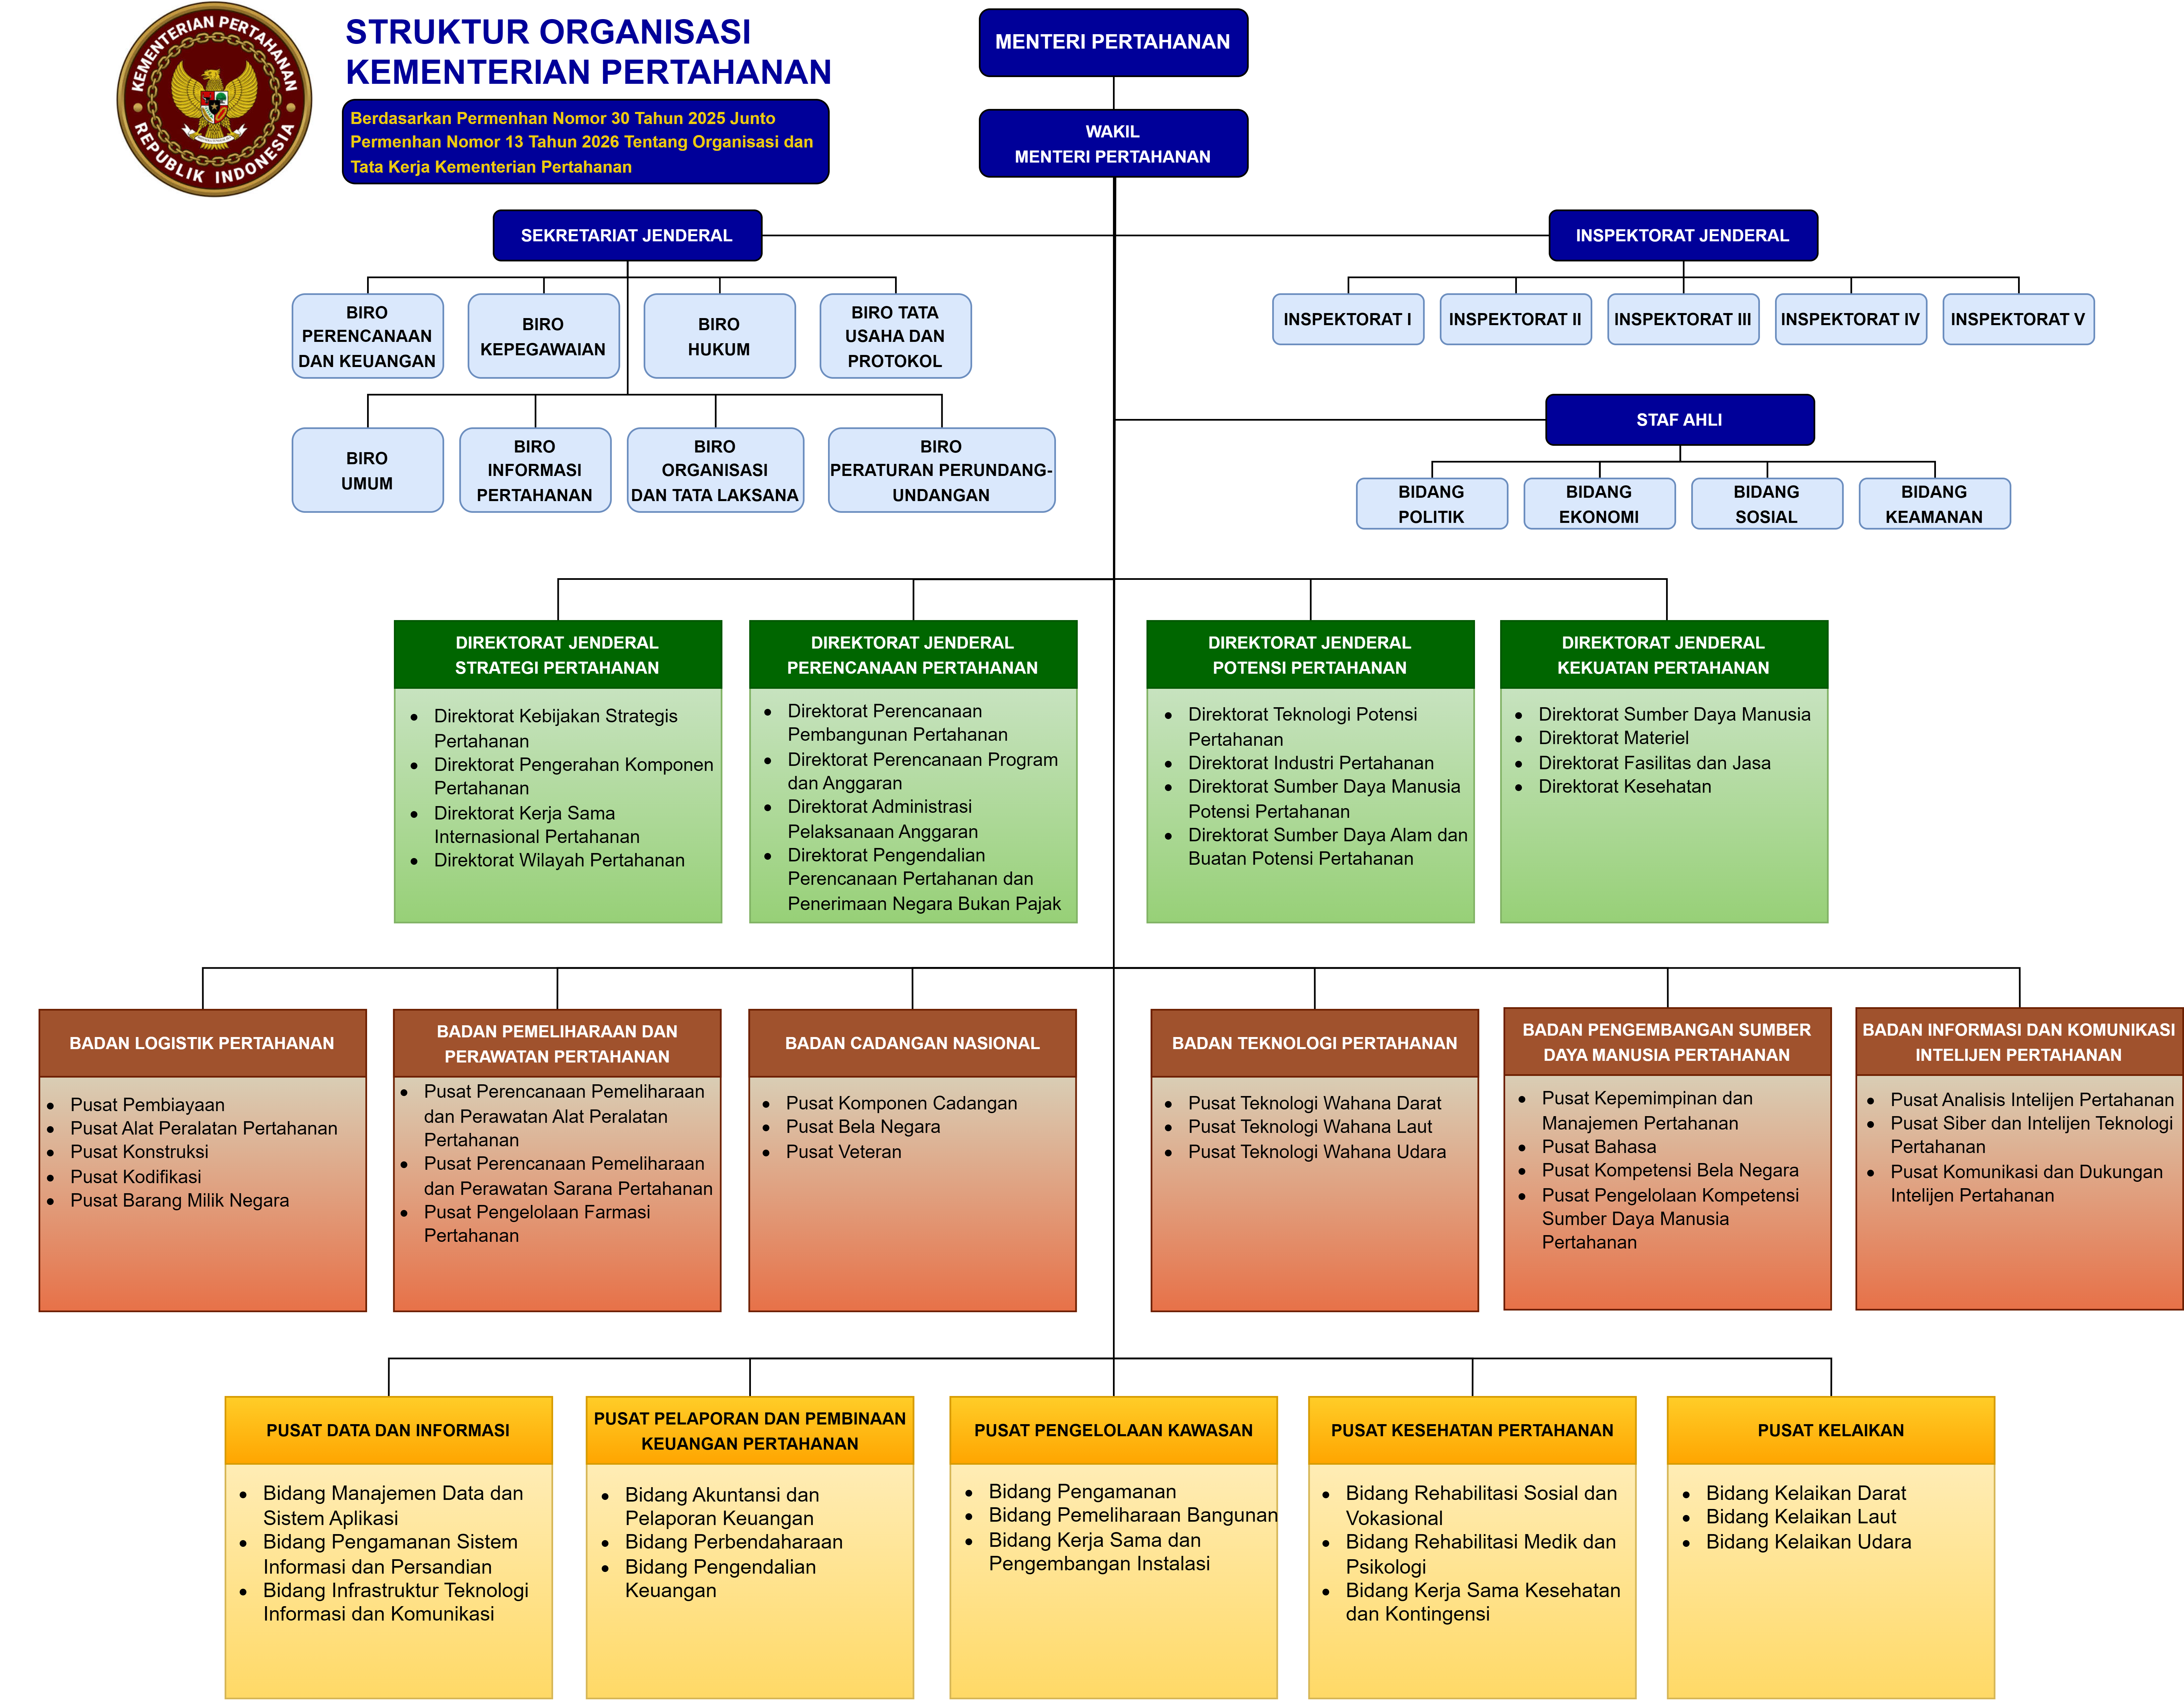
\includegraphics[width=1.00\linewidth,height=0.8\textheight,keepaspectratio]{images/Struktur Organisasi Kemhan Permenhan 30_2025 dan 13_2026.drawio.png}
\caption{Struktur Organisasi dan Tata Kerja Kemhan RI}
\label{fig:IV.4}
\end{figure}

Gambar~\ref{fig:IV.4} menunjukkan bahwa Kemhan RI dipimpin oleh Menteri Pertahanan yang dibantu Wakil Menteri Pertahanan. Unsur di bawahnya terdiri atas Sekretariat Jenderal, Inspektorat Jenderal, Staf Ahli, empat direktorat jenderal, enam badan, dan lima pusat. Fungsi utama setiap unit dirangkum pada Tabel~\ref{tab:IV.12}.

\begingroup\small\setstretch{1.0}
\begin{longtable}{@{}>{\raggedright\arraybackslash\hspace{0pt}}p{0.071\linewidth}>{\raggedright\arraybackslash\hspace{0pt}}p{0.343\linewidth}>{\raggedright\arraybackslash\hspace{0pt}}p{0.524\linewidth}@{}}
\caption{Fungsi Utama Unit Organisasi Kemhan RI}\label{tab:IV.12}\\
\toprule
\textbf{No.} & \textbf{Unit Organisasi} & \textbf{Fungsi Utama}\\
\midrule
\endfirsthead
\multicolumn{3}{@{}l}{\small\itshape \tablename\ \thetable{} (lanjutan)}\\
\toprule
\textbf{No.} & \textbf{Unit Organisasi} & \textbf{Fungsi Utama}\\
\midrule
\endhead
\bottomrule
\endlastfoot
\centering\arraybackslash 1 & Inspektorat Jenderal & Pengawasan intern di lingkungan Kemhan RI\\*
\centering\arraybackslash 2 & Sekretariat Jenderal & Koordinasi pelaksanaan tugas, pembinaan, dan dukungan administrasi seluruh unsur Kemhan RI\\
\centering\arraybackslash 3 & Staf Ahli & Rekomendasi atas isu strategis kepada Menteri sesuai bidangnya\\
\centering\arraybackslash 4 & Ditjen Strategi Pertahanan & Kebijakan di bidang strategi pertahanan\\
\centering\arraybackslash 5 & Ditjen Perencanaan Pertahanan & Kebijakan di bidang perencanaan pertahanan\\
\centering\arraybackslash 6 & Ditjen Potensi Pertahanan & Kebijakan di bidang potensi pertahanan, termasuk pembinaan industri pertahanan\\
\centering\arraybackslash 7 & Ditjen Kekuatan Pertahanan & Kebijakan di bidang kekuatan pertahanan\\
\centering\arraybackslash 8 & Badan Logistik Pertahanan & Pengelolaan logistik dan sarana pertahanan\\
\centering\arraybackslash 9 & Badan Pemeliharaan dan Perawatan Pertahanan & Pemeliharaan Alpalhankam dan sarana pertahanan serta koordinasi farmasi pertahanan\\
\centering\arraybackslash 10 & Badan Cadangan Nasional & Pembinaan komponen cadangan, bela negara, dan keveteranan\\
\centering\arraybackslash 11 & Badan Teknologi Pertahanan & Pengembangan teknologi wahana darat, laut, dan udara\\
\centering\arraybackslash 12 & Badan Pengembangan Sumber Daya Manusia Pertahanan & Pengembangan sumber daya manusia pertahanan\\
\centering\arraybackslash 13 & Badan Informasi dan Komunikasi Intelijen Pertahanan & Analisis intelijen, siber dan intelijen teknologi, serta komunikasi dan dukungan intelijen pertahanan\\
\centering\arraybackslash 14 & Pusat Data dan Informasi & Sistem informasi, infrastruktur TIK, pengamanan sistem informasi dan persandian, serta manajemen Satu Data Pertahanan\\
\centering\arraybackslash 15 & Pusat Pelaporan dan Pembinaan Keuangan Pertahanan & Pelaporan dan pembinaan pengelolaan keuangan pertahanan\\
\centering\arraybackslash 16 & Pusat Pengelolaan Kawasan & Pengamanan, pemeliharaan bangunan, serta kerja sama dan pengembangan instalasi kawasan\\
\centering\arraybackslash 17 & Pusat Kesehatan Pertahanan & Rehabilitasi pascacedera, penyandang disabilitas, dan kesehatan pertahanan\\*
\centering\arraybackslash 18 & Pusat Kelaikan & Sertifikasi kelaikan Alpalhankam, konstruksi, satwa, dan fasilitas pertahanan\\
\end{longtable}
\endgroup

Tabel~\ref{tab:IV.12} menunjukkan bahwa fungsi data, sistem informasi, dan infrastruktur TIK berada pada Pusat Data dan Informasi, sedangkan fungsi siber dan intelijen teknologi berada pada Badan Informasi dan Komunikasi Intelijen Pertahanan. Pembagian peran Kemhan RI juga sesuai dengan entitas dan peran pada BRA (Tabel~\ref{tab:III.12}). Kemhan RI berperan sebagai penetap kebijakan, standar, dan pengelola sumber daya pertahanan, sedangkan penggunaan kekuatan berada pada Mabes TNI \cite{UU3Tahun2025}.

Meskipun demikian, pengelolaan teknologi informasi dan data masih bersifat operasional pada masing-masing unit. Akibatnya, sistem berjalan terfragmentasi dan data tersilo antarunit. Kondisi ini menunjukkan bahwa struktur saat ini belum memiliki unit yang memegang mandat transformasi digital lintas organisasi.

\subsection{Value Stream}
\label{sec:IV.4.2}

Aliran nilai Kemhan RI diadopsi dari lima aliran nilai pada BRA tanpa perubahan, kemudian dijabarkan sesuai fungsi Kemhan RI. Aliran nilai tersebut menggambarkan penyelenggaraan pertahanan secara horizontal lintas unit, sebagaimana disajikan pada Gambar~\ref{fig:IV.5}.

\begin{figure}[htbp]
\centering
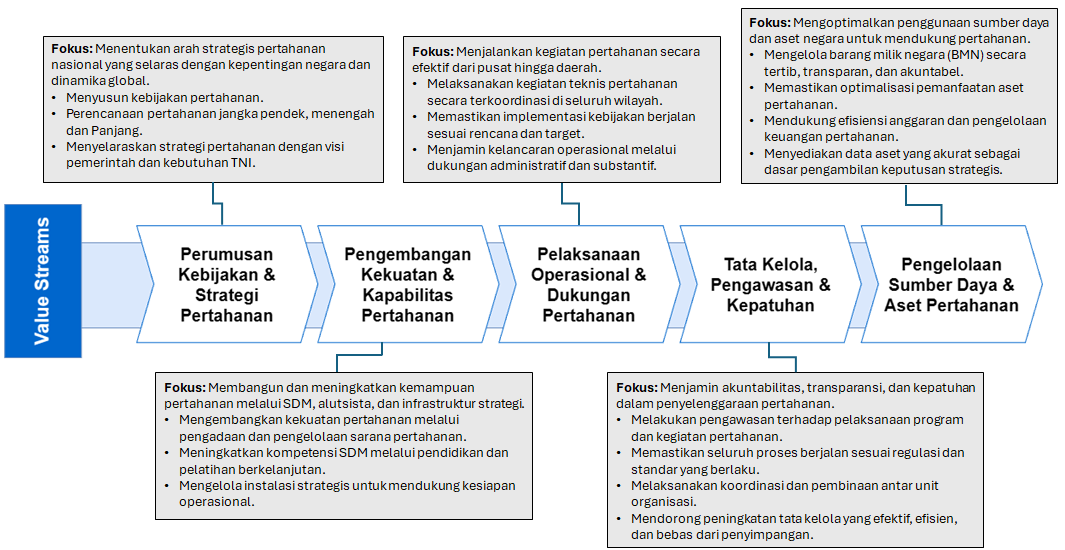
\includegraphics[width=1.00\linewidth,height=0.8\textheight,keepaspectratio]{images/Value Stream Kemhan dan Penjelasan.png}
\caption{\textit{Value Stream} Kemhan RI}
\label{fig:IV.5}
\end{figure}

Gambar~\ref{fig:IV.5} menunjukkan lima aliran nilai yang berurutan, yaitu:

\begin{enumerate}[label=\arabic*.]
\item Perumusan Kebijakan dan Strategi Pertahanan, yang menetapkan arah strategis serta perencanaan pertahanan jangka pendek, menengah, dan panjang;
\item Pengembangan Kekuatan dan Kapabilitas Pertahanan, yang membangun kemampuan melalui SDM, alutsista, dan infrastruktur strategis;
\item Pelaksanaan Operasional dan Dukungan Pertahanan, yang menjalankan kegiatan pertahanan secara terkoordinasi dari pusat hingga daerah;
\item Tata Kelola, Pengawasan, dan Kepatuhan, yang menjamin akuntabilitas, transparansi, dan kepatuhan terhadap regulasi; serta
\item Pengelolaan Sumber Daya dan Aset Pertahanan, yang mengoptimalkan barang milik negara, aset, dan keuangan pertahanan.
\end{enumerate}

Kelima aliran nilai tersebut menjadi dasar penurunan peta kapabilitas.

\subsection{Peta Kapabilitas}
\label{sec:IV.4.3}

Peta kapabilitas menjabarkan kemampuan yang diperlukan untuk menjalankan kelima aliran nilai. Pendekatan berbasis kapabilitas memisahkan “apa yang dilakukan” dari “siapa yang melakukannya”, sehingga arsitektur tetap stabil meskipun organisasi ditata ulang. Peta kapabilitas Kemhan RI pada kondisi \textit{baseline} disajikan pada Gambar~\ref{fig:IV.6}.

\begin{figure}[htbp]
\centering
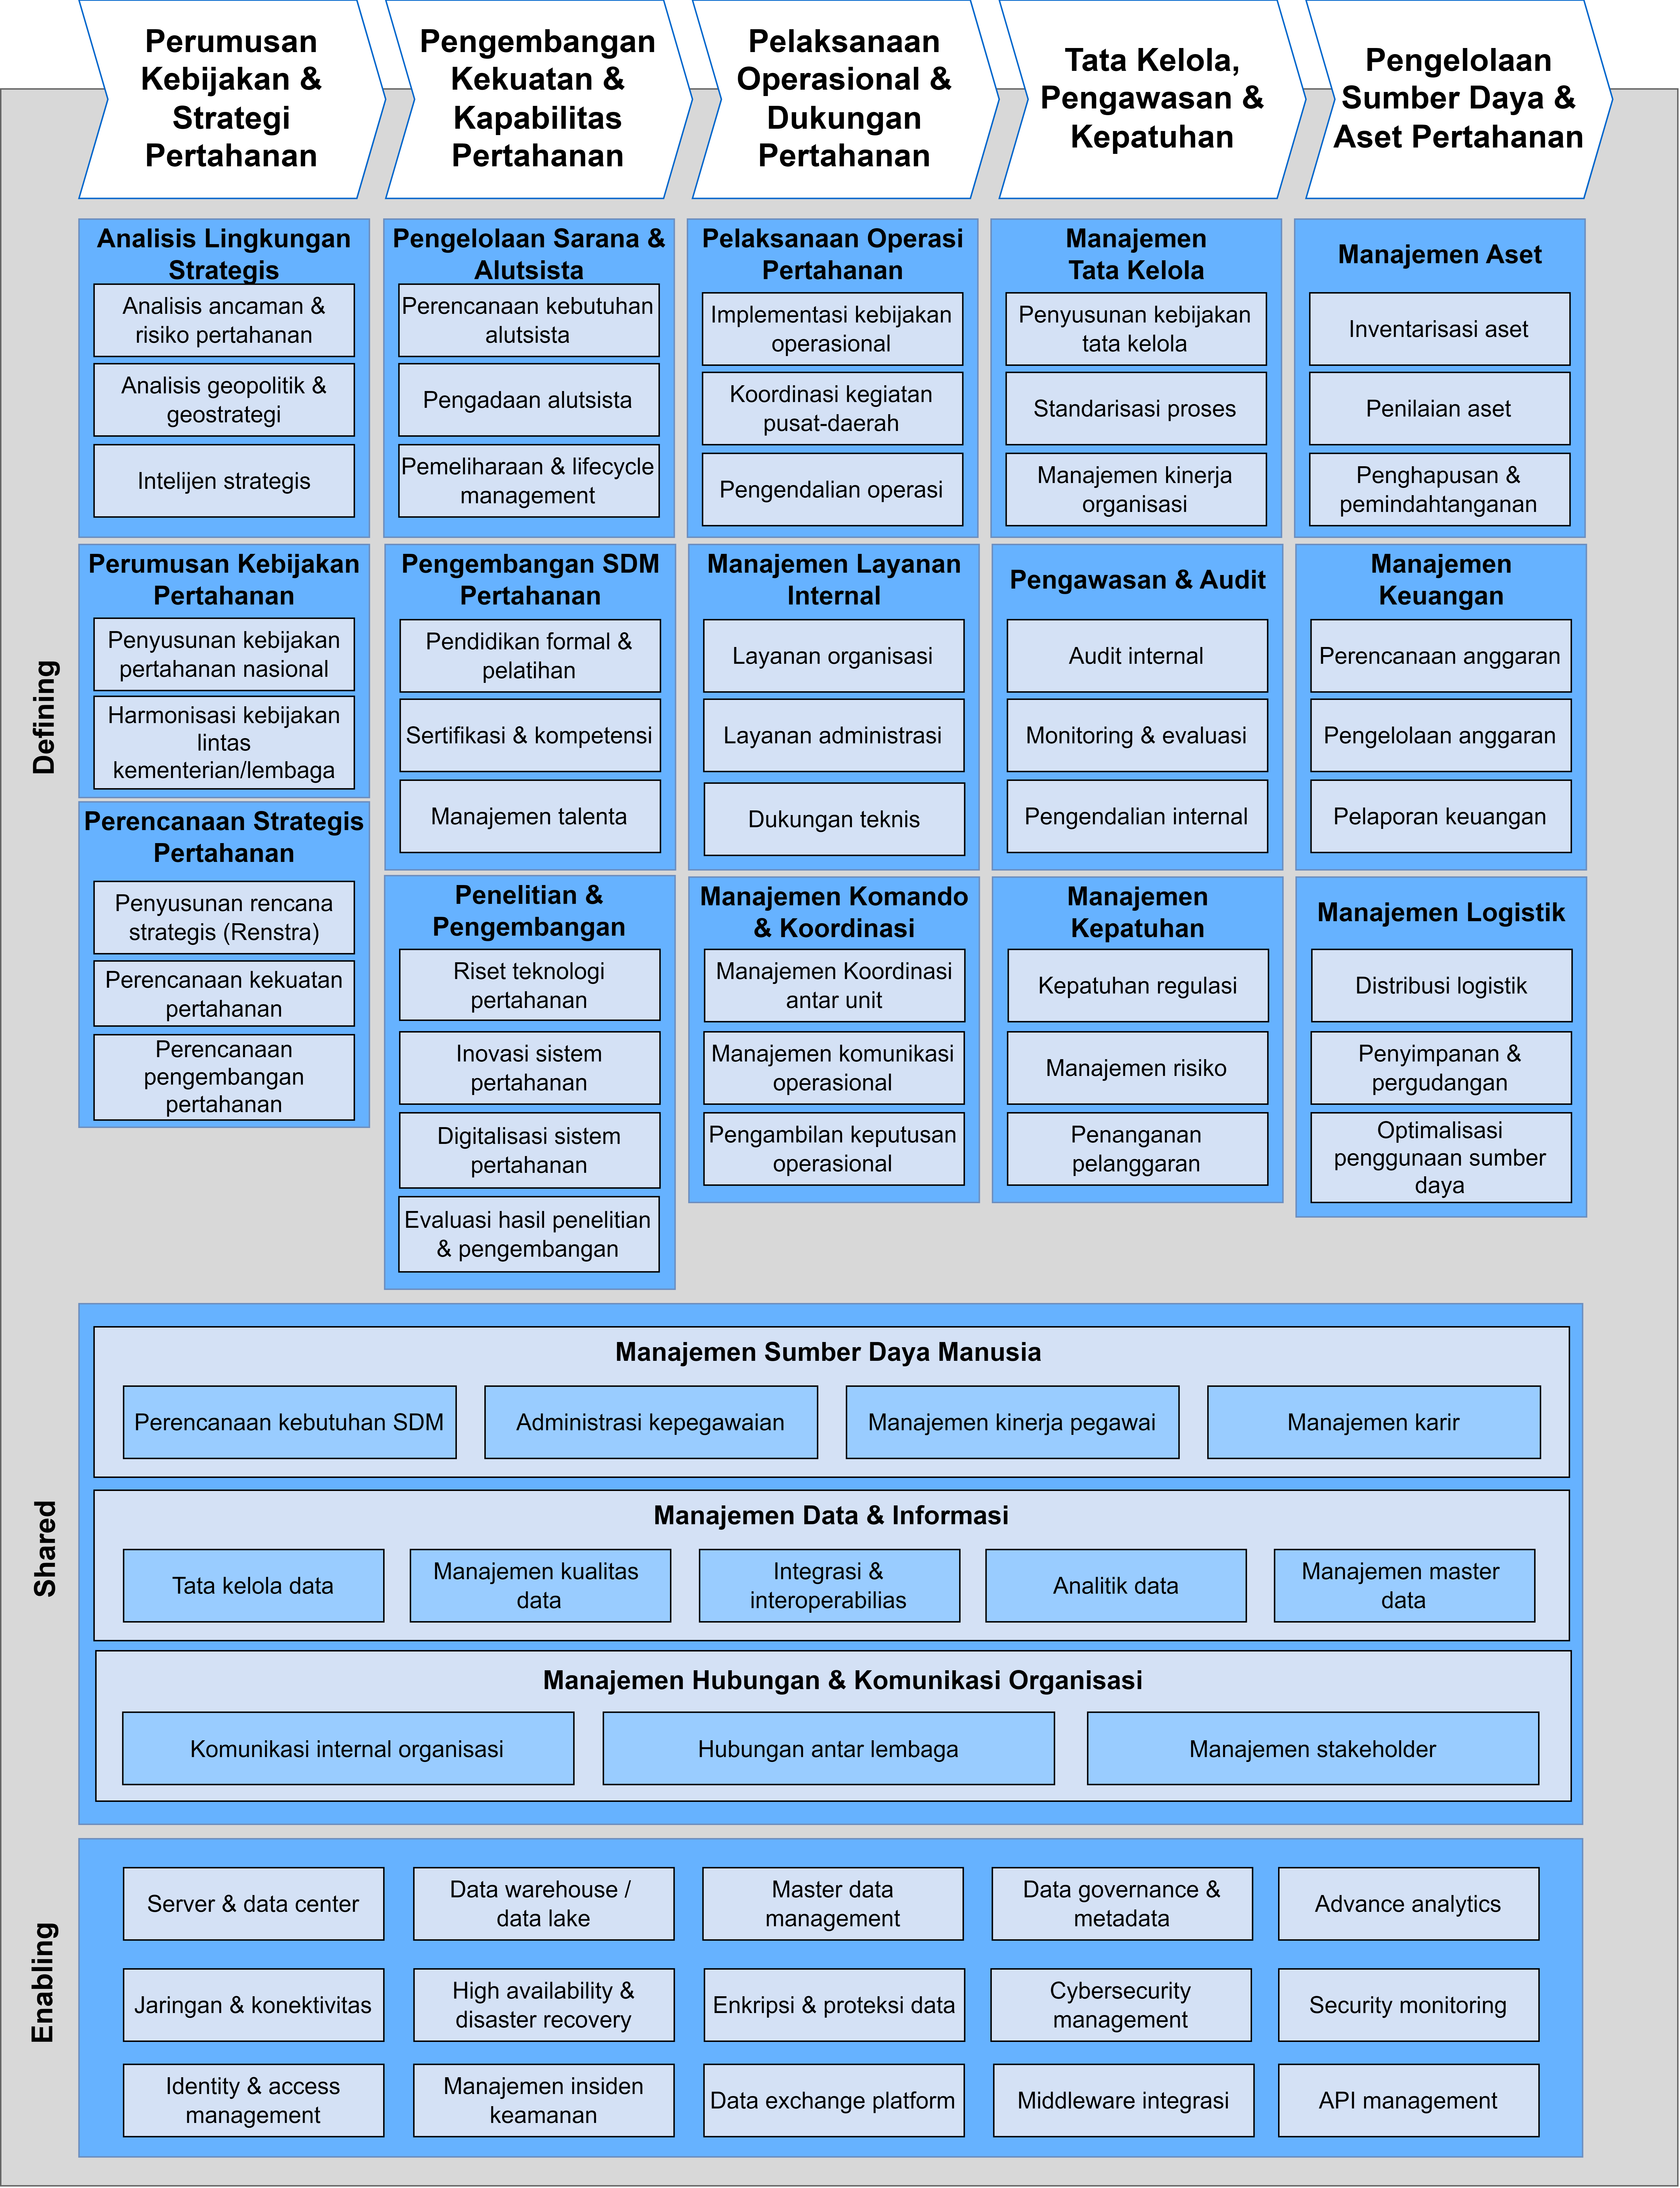
\includegraphics[width=0.93\linewidth,height=0.8\textheight,keepaspectratio]{images/Value Stream & Business Capability Map Kemhan.drawio.png}
\caption{\textit{Business Capability Map} Kemhan RI}
\label{fig:IV.6}
\end{figure}

Gambar~\ref{fig:IV.6} menyusun kapabilitas ke dalam tiga lapis. Lapis \textit{defining} memuat kapabilitas inti yang selaras dengan kelima aliran nilai. Lapis \textit{shared} memuat kapabilitas lintas fungsi, yaitu manajemen sumber daya manusia, manajemen data dan informasi, serta manajemen hubungan dan komunikasi organisasi. Lapis \textit{enabling} memuat fondasi teknologi. Untuk memenuhi KK-03, setiap kelompok kapabilitas dipetakan ke lapis CRM, sebagaimana disajikan pada Tabel~\ref{tab:IV.13}.

\begingroup\small\setstretch{1.0}
\begin{longtable}{@{}>{\raggedright\arraybackslash\hspace{0pt}}p{0.201\linewidth}>{\raggedright\arraybackslash\hspace{0pt}}p{0.477\linewidth}>{\raggedright\arraybackslash\hspace{0pt}}p{0.260\linewidth}@{}}
\caption{Pemetaan Peta Kapabilitas Kemhan RI ke CRM}\label{tab:IV.13}\\
\toprule
\textbf{Lapis CRM} & \textbf{Kelompok Kapabilitas Kemhan RI} & \textbf{Kapabilitas CRM Tanpa Padanan}\\
\midrule
\endfirsthead
\multicolumn{3}{@{}l}{\small\itshape \tablename\ \thetable{} (lanjutan)}\\
\toprule
\textbf{Lapis CRM} & \textbf{Kelompok Kapabilitas Kemhan RI} & \textbf{Kapabilitas CRM Tanpa Padanan}\\
\midrule
\endhead
\bottomrule
\endlastfoot
Strategis dan tata kelola & Analisis lingkungan strategis; perumusan kebijakan pertahanan; perencanaan strategis pertahanan; manajemen tata kelola; pengawasan dan audit; manajemen kepatuhan; manajemen hubungan dan komunikasi organisasi & Tata kelola arsitektur dan transformasi digital\\*
Operasional C6ISR & Pelaksanaan operasi pertahanan; manajemen komando dan koordinasi; intelijen strategis & Gambaran situasi bersama\\
Pengelolaan sumber daya pertahanan & Pengelolaan sarana dan alutsista; pengembangan SDM pertahanan; penelitian dan pengembangan; manajemen aset; manajemen keuangan; manajemen logistik; manajemen sumber daya manusia & \centering\arraybackslash –\\
Bersama & Manajemen layanan internal; manajemen data dan informasi; pusat data, gudang data, data induk, tata kelola data, analitik, ketersediaan tinggi dan pemulihan bencana, serta platform pertukaran data dan API & \centering\arraybackslash –\\*
Pendukung & Jaringan dan konektivitas; enkripsi; manajemen keamanan siber; pemantauan keamanan; manajemen identitas dan akses; manajemen insiden keamanan & Manajemen perubahan dan talenta digital\\
\end{longtable}
\endgroup

Tabel~\ref{tab:IV.13} menunjukkan bahwa seluruh kelompok kapabilitas Kemhan RI dapat dipetakan ke lapis CRM. Sebaliknya, terdapat tiga kapabilitas CRM yang belum memiliki padanan, yaitu kapabilitas yang berstatus belum tersedia pada Gambar~\ref{fig:IV.2}. Dengan demikian, CRM berfungsi sebagai alat untuk menemukan kapabilitas yang hilang pada peta kapabilitas organisasi.

\subsection{Arsitektur Bisnis Target}
\label{sec:IV.4.4}

Arsitektur bisnis target difokuskan pada penutupan tiga kapabilitas yang belum tersedia. Dua di antaranya, yaitu tata kelola arsitektur dan transformasi digital serta manajemen perubahan dan talenta digital, memerlukan perubahan struktur organisasi dan peta kapabilitas. Kapabilitas gambaran situasi bersama dikelola bersama Mabes TNI, sehingga kontribusi Kemhan RI diwujudkan melalui arsitektur data, aplikasi, dan teknologi pada Fase C dan D.

\subsubsection{Struktur Organisasi Target}
\label{sec:IV.4.4.1}

Berdasarkan Gambar~\ref{fig:IV.4} dan Tabel~\ref{tab:IV.13}, terdapat lima fungsi strategis transformasi digital yang belum memiliki penanggung jawab, yaitu:

\begin{enumerate}[label=\arabic*.]
\item perumusan strategi dan \textit{roadmap} transformasi digital pertahanan;
\item tata kelola arsitektur enterprise, termasuk pengelolaan DERA, serta standardisasi sistem lintas unit dan lintas matra;
\item koordinasi transformasi digital lintas satuan kerja dan lintas matra;
\item tata kelola data sebagai aset strategis, melampaui pengelolaan data yang bersifat operasional; dan
\item pengkajian dan adopsi teknologi baru, seperti kecerdasan buatan dan komputasi awan.
\end{enumerate}

Kelima fungsi tersebut diampu oleh unit \textit{Digital Transformation Officer} (DTO\label{sk:DTO}) yang dipimpin CDTO dan bertanggung jawab langsung kepada Menteri Pertahanan. Kedudukan ini memberikan kewenangan lintas eselon I dan lintas matra, memisahkan DTO dari fungsi operasional Pusat Data dan Informasi, serta memungkinkan CDTO memimpin \textit{Architecture Board}. Struktur organisasi target disajikan pada Gambar~\ref{fig:IV.7}.

\begin{figure}[htbp]
\centering
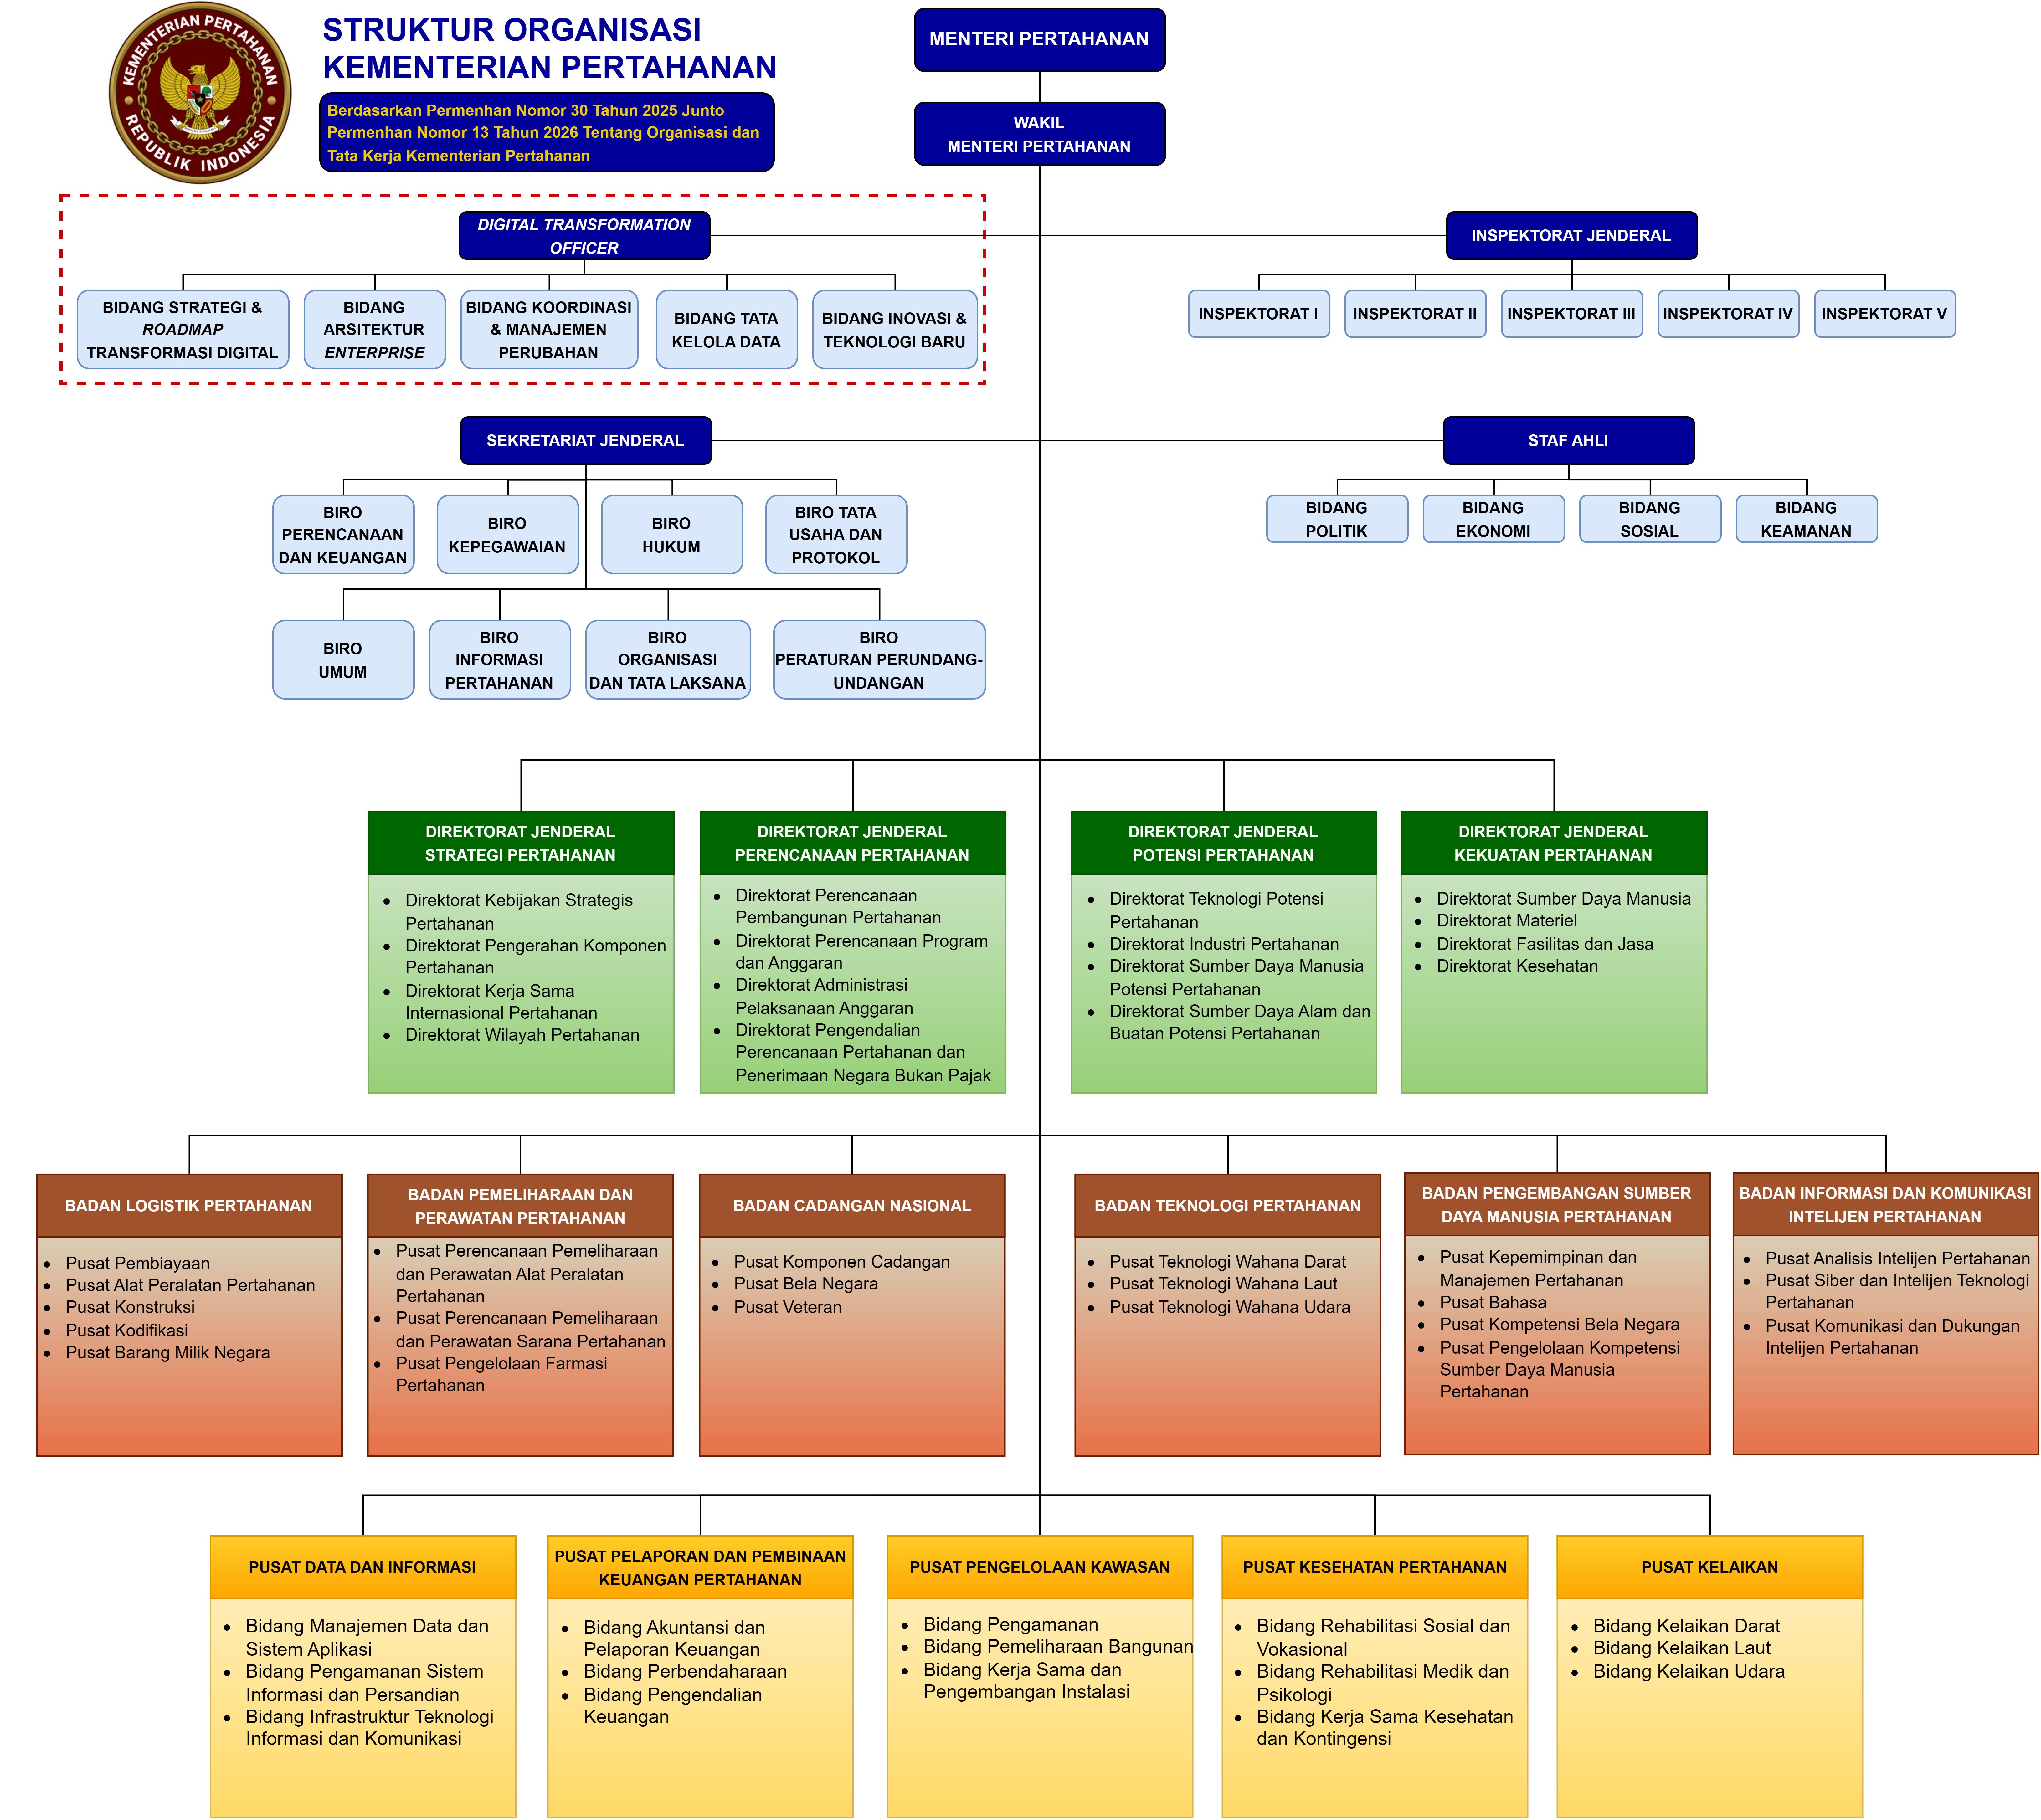
\includegraphics[width=1.00\linewidth,height=0.8\textheight,keepaspectratio]{images/Struktur Organisasi Kemhan Permenhan 30_2025 dan 13_2026 To Be.drawio.png}
\caption{Struktur Organisasi \textit{To-Be} Kemhan RI}
\label{fig:IV.7}
\end{figure}

Gambar~\ref{fig:IV.7} menunjukkan unit DTO (kotak bergaris putus merah) yang berkedudukan langsung di bawah Menteri Pertahanan. Unit ini terdiri atas lima bidang yang masing-masing mengampu satu fungsi strategis di atas, yaitu:

\begin{enumerate}[label=\arabic*.]
\item Bidang Strategi dan \textit{Roadmap} Transformasi Digital, yang merumuskan strategi dan \textit{roadmap} transformasi digital serta memantau capaiannya;
\item Bidang Arsitektur \textit{Enterprise}, yang memelihara DERA dan EA Kemhan RI, menetapkan standar sistem lintas unit dan lintas matra, serta menyiapkan bahan keputusan \textit{Architecture Board};
\item Bidang Koordinasi dan Manajemen Perubahan, yang mengoordinasikan transformasi lintas satuan kerja dan lintas matra serta mengelola kesiapan organisasi;
\item Bidang Tata Kelola Data, yang menetapkan kebijakan, standar, dan kepemilikan data pertahanan, sedangkan pengelolaan teknisnya tetap dilaksanakan Pusat Data dan Informasi selaku walidata; serta
\item Bidang Inovasi dan Teknologi Baru, yang mengkaji teknologi baru dan menyiapkan adopsinya melalui uji coba terbatas.
\end{enumerate}

DTO menetapkan arah strategi dan arsitektur, sedangkan Pusat Data dan Informasi tetap menjadi pelaksana di bidang data, sistem informasi, dan infrastruktur TIK. Dengan demikian, DTO memperkuat, bukan menggantikan, unit yang telah ada.

\subsubsection{Peta Kapabilitas Target}
\label{sec:IV.4.4.2}

Peta kapabilitas target merupakan pemutakhiran atas Gambar~\ref{fig:IV.6} dengan menambahkan kapabilitas yang belum memiliki padanan pada Tabel~\ref{tab:IV.13}. Karena bersifat lintas fungsi, kapabilitas baru ditempatkan pada lapis \textit{shared}, sebagaimana disajikan pada Gambar~\ref{fig:IV.8}.

\begin{figure}[htbp]
\centering
\includegraphics[width=0.93\linewidth,height=0.8\textheight,keepaspectratio]{images/Value Stream & Business Capability Map Kemhan To-Be.drawio.png}
\caption{\textit{Business Capability Map} Kemhan RI \textit{To-Be}}
\label{fig:IV.8}
\end{figure}

Gambar~\ref{fig:IV.8} menunjukkan tiga tambahan kapabilitas yang ditandai warna hijau, yaitu:

\begin{enumerate}[label=\arabic*.]
\item Tata Kelola Arsitektur \textit{Enterprise}, sebagai padanan kapabilitas tata kelola arsitektur dan transformasi digital pada CRM;
\item Manajemen Perubahan, yang mencakup manajemen perubahan organisasi, adopsi dan komunikasi perubahan, serta kesiapan transformasi; dan
\item Manajemen Talenta Digital, sebagai subkapabilitas manajemen sumber daya manusia.
\end{enumerate}

Tambahan kedua dan ketiga merupakan padanan kapabilitas manajemen perubahan dan talenta digital pada CRM. Dengan tambahan tersebut, seluruh kapabilitas CRM dalam cakupan Kemhan RI memiliki padanan, kecuali gambaran situasi bersama yang ditindaklanjuti pada Fase C dan D.

\subsubsection{Analisis Kesenjangan}
\label{sec:IV.4.4.3}

Analisis kesenjangan membandingkan kondisi \textit{baseline} dengan arsitektur bisnis target. Hasilnya disajikan pada Tabel~\ref{tab:IV.14}.

\begingroup\small\setstretch{1.0}
\begin{longtable}{@{}>{\raggedright\arraybackslash\hspace{0pt}}p{0.066\linewidth}>{\raggedright\arraybackslash\hspace{0pt}}p{0.177\linewidth}>{\raggedright\arraybackslash\hspace{0pt}}p{0.210\linewidth}>{\raggedright\arraybackslash\hspace{0pt}}p{0.213\linewidth}>{\raggedright\arraybackslash\hspace{0pt}}p{0.210\linewidth}@{}}
\caption{Analisis Kesenjangan Arsitektur Bisnis}\label{tab:IV.14}\\
\toprule
\textbf{No.} & \textbf{Aspek} & \textbf{Kondisi \textit{Baseline}} & \textbf{Kondisi Target} & \textbf{Tindak Lanjut}\\
\midrule
\endfirsthead
\multicolumn{5}{@{}l}{\small\itshape \tablename\ \thetable{} (lanjutan)}\\
\toprule
\textbf{No.} & \textbf{Aspek} & \textbf{Kondisi \textit{Baseline}} & \textbf{Kondisi Target} & \textbf{Tindak Lanjut}\\
\midrule
\endhead
\bottomrule
\endlastfoot
\centering\arraybackslash 1 & Struktur dan mandat transformasi & Belum ada unit bermandat transformasi digital lintas organisasi & Unit DTO pada tingkat strategis dengan lima bidang & Pembentukan unit DTO\\*
\centering\arraybackslash 2 & Tata kelola arsitektur & Belum ada tata kelola arsitektur dan standar lintas unit & Kapabilitas Tata Kelola Arsitektur \textit{Enterprise} dan \textit{Architecture Board} & Penetapan tata kelola dan adopsi DERA\\
\centering\arraybackslash 3 & Manajemen perubahan & Transformasi berjalan parsial tanpa pengelolaan perubahan & Kapabilitas Manajemen Perubahan yang terlembaga & Pembangunan kapabilitas manajemen perubahan\\
\centering\arraybackslash 4 & Proses bisnis lintas unit & Proses terfragmentasi dan belum terstandar antarunit & Proses terstandar dan terintegrasi berbasis kapabilitas & Standardisasi dan integrasi proses bisnis\\
\centering\arraybackslash 5 & Koordinasi lintas matra & Koordinasi antarunit dan antarmatra bersifat \textit{ad hoc} & Mekanisme koordinasi transformasi lintas matra yang terlembaga & Penetapan mekanisme koordinasi lintas matra\\
\centering\arraybackslash 6 & Talenta digital & Kompetensi digital terbatas dan tersebar antarunit & Kapabilitas Manajemen Talenta Digital & Pengembangan dan rekrutmen talenta digital\\*
\centering\arraybackslash 7 & Antarmuka C6ISR & Gambaran situasi bersama dengan Mabes TNI belum tersedia & Kebijakan dan standar pertukaran data untuk gambaran situasi bersama sesuai hak akses & Ditindaklanjuti pada Fase C dan D melalui pola P2 dan P6\\
\end{longtable}
\endgroup

Tabel~\ref{tab:IV.14} menunjukkan bahwa kesenjangan 1 dan 2 bersifat struktural, sehingga harus ditutup lebih dahulu sebagai prasyarat bagi kesenjangan lainnya.

\section{Fase C: Information Systems Architectures}
\label{sec:IV.5}

Fase \textit{Information Systems Architectures} merancang arsitektur data dan aplikasi yang mendukung arsitektur bisnis target. Pada langkah \textit{Select Reference Models, Viewpoints, and Tools}, DRA dan ARA dipilih sebagai model referensi. Arsitektur data dikerjakan lebih dahulu, kemudian arsitektur aplikasi. Keduanya bertolak dari inventarisasi aplikasi Kemhan RI tahun 2025 yang mencatat 247 aplikasi, terdiri atas 176 aplikasi umum dan 71 aplikasi khusus.

\subsection{Data Architecture}
\label{sec:IV.5.1}

Data Pertahanan adalah data yang dibina dan diselenggarakan oleh Kemhan RI dan TNI untuk kepentingan penyelenggaraan pertahanan negara. Aplikasi umum merupakan sistem nasional yang digunakan bersama oleh banyak instansi, sehingga datanya tunduk pada tata kelola instansi penyelenggaranya. Oleh karena itu, lingkup arsitektur data Kemhan RI adalah data pada 71 aplikasi khusus.

\subsubsection{Arsitektur Data Baseline}
\label{sec:IV.5.1.1}

Entitas data diturunkan dari fungsi 71 aplikasi khusus, kemudian dikelompokkan ke dalam area subjek DRA (Tabel~\ref{tab:III.13}). Hasil pengelompokan disajikan pada Tabel~\ref{tab:IV.15}.

\begingroup\small\setstretch{1.0}
\begin{longtable}{@{}>{\raggedright\arraybackslash\hspace{0pt}}p{0.248\linewidth}>{\raggedright\arraybackslash\hspace{0pt}}p{0.477\linewidth}>{\raggedright\arraybackslash\hspace{0pt}}p{0.213\linewidth}@{}}
\caption{Pemetaan Entitas Data Pertahanan ke Area Subjek DRA}\label{tab:IV.15}\\
\toprule
\textbf{Area Subjek DRA} & \textbf{Entitas Data Kemhan RI} & \textbf{Klasifikasi Acuan}\\
\midrule
\endfirsthead
\multicolumn{3}{@{}l}{\small\itshape \tablename\ \thetable{} (lanjutan)}\\
\toprule
\textbf{Area Subjek DRA} & \textbf{Entitas Data Kemhan RI} & \textbf{Klasifikasi Acuan}\\
\midrule
\endhead
\bottomrule
\endlastfoot
Kebijakan dan strategi & \centering\arraybackslash – & Terbatas–Rahasia\\*
Personel & Kinerja pegawai; kompetensi dan asesmen; kartu identitas pegawai; veteran & Terbatas\\
Anggaran dan keuangan & Pelaporan keuangan internal & Terbuka–Terbatas\\
Materiil dan alutsista & Penelitian dan pengembangan & Terbatas–Rahasia\\
Operasi dan situasi & \centering\arraybackslash – & Rahasia\\
Intelijen dan ISR & \centering\arraybackslash – & Rahasia\\
Geospasial & Geospasial wilayah pertahanan & Terbuka–Rahasia\\
Infrastruktur dan TIK & Log dan insiden keamanan siber; identitas dan kendali akses; aset dan infrastruktur TIK & Terbatas\\
Industri pertahanan & Sumber daya dan industri pertahanan; perizinan pertahanan & Terbuka–Terbatas\\
Informasi publik & Layanan informasi publik & Terbuka\\
Hukum dan pengawasan (perluasan) & Perkara dan dokumentasi hukum; pengawasan intern & Terbatas\\*
Pendidikan dan kesehatan (perluasan) & Peserta didik dan akademik; alumni; bahan ajar dan pembelajaran digital; rekam medis dan pasien; klaim layanan kesehatan & Terbatas\\
\end{longtable}
\endgroup

Tabel~\ref{tab:IV.15} menunjukkan tiga temuan. Pertama, dua area subjek ditambahkan sebagai perluasan DRA, yaitu hukum dan pengawasan serta pendidikan dan kesehatan, sesuai mekanisme penyesuaian pada III.5.3. Kedua, area kebijakan dan strategi tidak memiliki entitas pada aplikasi khusus karena datanya dikelola melalui aplikasi umum. Ketiga, area operasi dan situasi serta intelijen dan ISR belum memiliki entitas, sehingga pertukaran data C6ISR dengan Mabes TNI belum didukung. Selain itu, satu entitas dapat bersumber dari lebih dari satu aplikasi, sedangkan kamus data, klasifikasi, dan kanal berbagi-pakai belum tersedia.

\subsubsection{Klasifikasi dan Tata Kelola Data}
\label{sec:IV.5.1.2}

Klasifikasi data menyeimbangkan kewajiban berbagi-pakai data dengan kewajiban kerahasiaan pertahanan. Sesuai Pasal 21 Permenhan Nomor 1 Tahun 2023 \cite{Permenhan1Tahun2023}, Data Pertahanan diklasifikasikan ke dalam tiga tingkat, sebagaimana disajikan pada Tabel~\ref{tab:IV.16}.

\begingroup\small\setstretch{1.0}
\begin{longtable}{@{}>{\raggedright\arraybackslash\hspace{0pt}}p{0.177\linewidth}>{\raggedright\arraybackslash\hspace{0pt}}p{0.418\linewidth}>{\raggedright\arraybackslash\hspace{0pt}}p{0.343\linewidth}@{}}
\caption{Klasifikasi Data Pertahanan}\label{tab:IV.16}\\
\toprule
\textbf{Klasifikasi} & \textbf{Kriteria} & \textbf{Kendali Akses}\\
\midrule
\endfirsthead
\multicolumn{3}{@{}l}{\small\itshape \tablename\ \thetable{} (lanjutan)}\\
\toprule
\textbf{Klasifikasi} & \textbf{Kriteria} & \textbf{Kendali Akses}\\
\midrule
\endhead
\bottomrule
\endlastfoot
Terbuka & Data yang boleh diketahui publik & Terbuka bagi publik melalui Portal Satu Data Pertahanan\\*
Terbatas & Data yang hanya dapat diakses kementerian/lembaga yang diberi akses oleh Walidata Pertahanan & Otentikasi dan hak akses berbasis izin Walidata Pertahanan\\*
Rahasia & Data yang hanya dapat diakses pejabat berwenang di Kemhan RI, Mabes TNI, dan Mabes Angkatan & Otorisasi khusus, enkripsi, pencatatan audit, dan pemrosesan pada domain operasional terklasifikasi\\
\end{longtable}
\endgroup

Tabel~\ref{tab:IV.16} menunjukkan bahwa klasifikasi Rahasia diproses pada domain operasional terklasifikasi sesuai pola P5. Setiap entitas juga dicatat dalam kamus data yang memuat definisi baku entitas dan atribut, sedangkan metadata melekat pada setiap set data mengikuti struktur Satu Data Indonesia \cite{Perpres39Tahun2019}. Tata kelola Data Pertahanan mengikuti peran penyelenggara Satu Data Pertahanan \cite{Permenhan1Tahun2023}, sebagaimana disajikan pada Tabel~\ref{tab:IV.17}.

\begingroup\small\setstretch{1.0}
\begin{longtable}{@{}>{\raggedright\arraybackslash\hspace{0pt}}p{0.225\linewidth}>{\raggedright\arraybackslash\hspace{0pt}}p{0.406\linewidth}>{\raggedright\arraybackslash\hspace{0pt}}p{0.307\linewidth}@{}}
\caption{Peran Penyelenggara Satu Data Pertahanan}\label{tab:IV.17}\\
\toprule
\textbf{Peran} & \textbf{Tugas Pokok} & \textbf{Pemangku Peran}\\
\midrule
\endfirsthead
\multicolumn{3}{@{}l}{\small\itshape \tablename\ \thetable{} (lanjutan)}\\
\toprule
\textbf{Peran} & \textbf{Tugas Pokok} & \textbf{Pemangku Peran}\\
\midrule
\endhead
\bottomrule
\endlastfoot
Pengarah & Mengoordinasikan pelaksanaan, pemantauan, evaluasi, dan pelaporan Satu Data Pertahanan kepada Menteri & Sekretaris Jenderal\\*
Walidata Pertahanan & Merencanakan, mengumpulkan, memeriksa, mengelola, dan menyebarluaskan data melalui Portal Satu Data Pertahanan & Pusat Data dan Informasi\\
Produsen Data Pertahanan & Menghasilkan data sesuai prinsip Satu Data serta menyampaikan data dan metadata kepada walidata & Satuan kerja penghasil data di Kemhan RI dan Mabes TNI\\
Pengolah Data Pertahanan & Mendistribusikan Data Pertahanan hingga sampai kepada walidata & Satuan kerja pengelola data di Mabes Angkatan\\*
Pengaman Sistem Data Pertahanan & Mengamankan, memantau, menguji, dan merespons ancaman siber terhadap sistem Satu Data Pertahanan & Bidang Pengamanan Sistem Informasi dan Persandian, didukung Pusat Siber dan Intelijen Teknologi Pertahanan\\
\end{longtable}
\endgroup

Tabel~\ref{tab:IV.17} menunjukkan bahwa data dihasilkan oleh produsen data di satuan kerja, sedangkan pengelolaan dan penyebarluasannya dipusatkan pada Walidata Pertahanan. Kebijakan dan standar data ditetapkan oleh Bidang Tata Kelola Data pada unit DTO, kemudian dijalankan oleh walidata.

\subsubsection{Arsitektur Data Target}
\label{sec:IV.5.1.3}

Arsitektur data target adalah terwujudnya Satu Data Pertahanan, yaitu Data Pertahanan yang terstandar, terklasifikasi, dimiliki secara jelas, aman, dan dapat dibagipakaikan secara terkendali. Arsitektur ini disusun dalam tiga lapis, yaitu fondasi, platform, dan target, sebagaimana ditunjukkan pada Gambar~\ref{fig:IV.9}.

\begin{figure}[htbp]
\centering
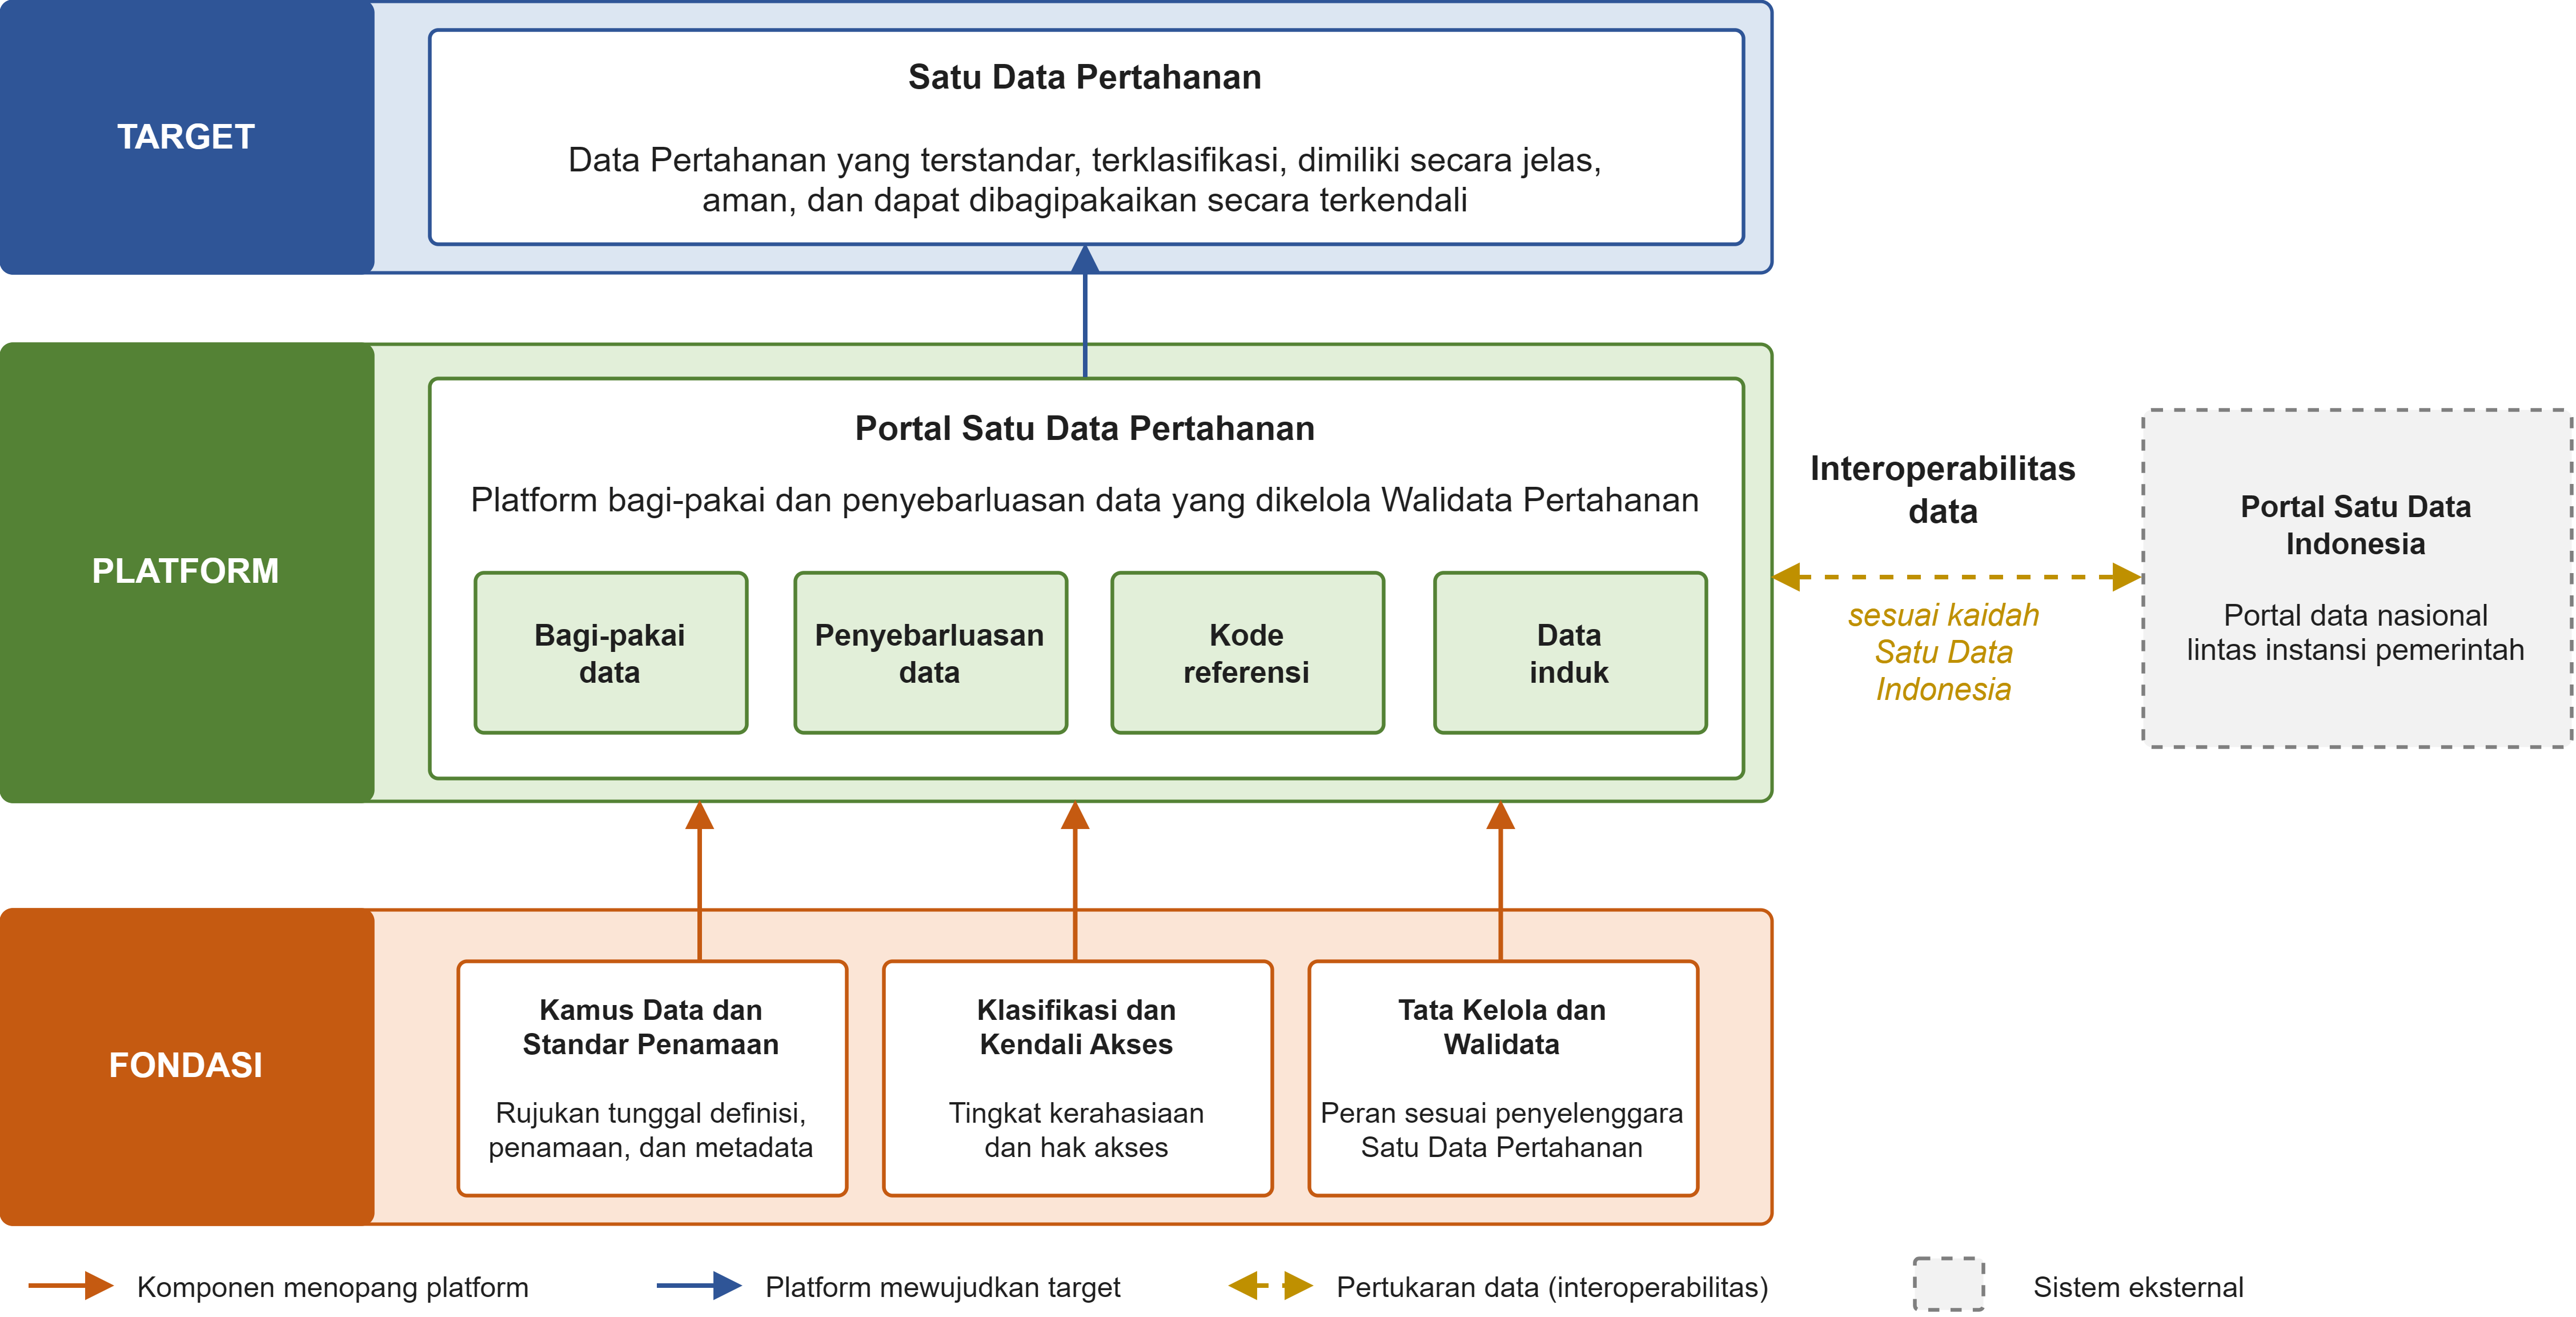
\includegraphics[width=1.00\linewidth,height=0.8\textheight,keepaspectratio]{images/Arsitektur_Data_Target.drawio.png}
\caption{Arsitektur Data Target}
\label{fig:IV.9}
\end{figure}

Gambar~\ref{fig:IV.9} menunjukkan bahwa lapis fondasi terdiri atas kamus data dan standar penamaan, klasifikasi dan kendali akses, serta tata kelola dan walidata. Lapis platform adalah Portal Satu Data Pertahanan (ABB-03) dengan fungsi bagi-pakai data, penyebarluasan data, kode referensi, dan data induk. Portal ini terhubung dengan Portal Satu Data Indonesia hanya untuk data yang klasifikasinya memungkinkan. Data operasi dan intelijen tetap berada pada domain operasional terklasifikasi, sedangkan Kemhan RI menerima data situasi tingkat strategis melalui gerbang lintas domain sesuai pola P5 dan P6.

\subsubsection{Analisis Kesenjangan Data}
\label{sec:IV.5.1.4}

Analisis kesenjangan arsitektur data disajikan pada Tabel~\ref{tab:IV.18}.

\begingroup\small\setstretch{1.0}
\begin{longtable}{@{}>{\raggedright\arraybackslash\hspace{0pt}}p{0.066\linewidth}>{\raggedright\arraybackslash\hspace{0pt}}p{0.177\linewidth}>{\raggedright\arraybackslash\hspace{0pt}}p{0.210\linewidth}>{\raggedright\arraybackslash\hspace{0pt}}p{0.213\linewidth}>{\raggedright\arraybackslash\hspace{0pt}}p{0.210\linewidth}@{}}
\caption{Analisis Kesenjangan Arsitektur Data}\label{tab:IV.18}\\
\toprule
\textbf{No.} & \textbf{Aspek} & \textbf{Kondisi \textit{Baseline}} & \textbf{Kondisi Target} & \textbf{Tindak Lanjut}\\
\midrule
\endfirsthead
\multicolumn{5}{@{}l}{\small\itshape \tablename\ \thetable{} (lanjutan)}\\
\toprule
\textbf{No.} & \textbf{Aspek} & \textbf{Kondisi \textit{Baseline}} & \textbf{Kondisi Target} & \textbf{Tindak Lanjut}\\
\midrule
\endhead
\bottomrule
\endlastfoot
\centering\arraybackslash 1 & Standar dan definisi data & Definisi dan penamaan berbeda antaraplikasi & Kamus data dan standar penamaan yang seragam & Penetapan kamus data dan standar penamaan\\*
\centering\arraybackslash 2 & Integrasi dan berbagi-pakai & Data terkotak per aplikasi dan satuan kerja & Berbagi-pakai melalui Portal Satu Data Pertahanan & Pembangunan Portal Satu Data Pertahanan\\
\centering\arraybackslash 3 & Tata kelola dan kepemilikan & Belum ada walidata dan produsen data yang baku & Walidata dan produsen data sesuai Permenhan 1/2023 & Penetapan penyelenggara Satu Data Pertahanan\\
\centering\arraybackslash 4 & Klasifikasi & Belum ada klasifikasi yang tegas & Tiga tingkat klasifikasi & Penetapan dan penerapan klasifikasi data\\
\centering\arraybackslash 5 & Keamanan dan akses & Kendali akses parsial per aplikasi & Kendali akses berbasis klasifikasi & Penerapan kendali akses dan pengamanan sistem data\\
\centering\arraybackslash 6 & Interoperabilitas nasional & Pertukaran data manual atau terbatas & Interoperabilitas dengan Portal Satu Data Indonesia & Penetapan kode referensi, data induk, dan kaidah interoperabilitas\\*
\centering\arraybackslash 7 & Data C6ISR & Belum ada pertukaran data situasi dengan Mabes TNI & Pertukaran data situasi tingkat strategis melalui gerbang lintas domain & Penetapan standar pertukaran data bersama Mabes TNI\\
\end{longtable}
\endgroup

Tabel~\ref{tab:IV.18} menunjukkan bahwa kesenjangan 1, 3, 4, dan 7 dapat ditutup melalui penetapan kebijakan dan standar, sedangkan kesenjangan 2, 5, dan 6 memerlukan pembangunan platform.

\subsection{Application Architecture}
\label{sec:IV.5.2}

Arsitektur aplikasi merancang portofolio aplikasi yang mendukung proses bisnis dan arsitektur data target. Aplikasi umum digunakan sesuai ketentuan pemiliknya dan tidak dikembangkan ulang \cite{Perpres95Tahun2018}, sehingga perancangan difokuskan pada 71 aplikasi khusus.

\subsubsection{Arsitektur Aplikasi Baseline dan Rasionalisasi}
\label{sec:IV.5.2.1}

Pada kondisi \textit{baseline}, ke-71 aplikasi khusus berdiri sendiri per satuan kerja tanpa integrasi terpusat, sebagaimana ditunjukkan pada Gambar~\ref{fig:IV.10}.

\begin{figure}[htbp]
\centering
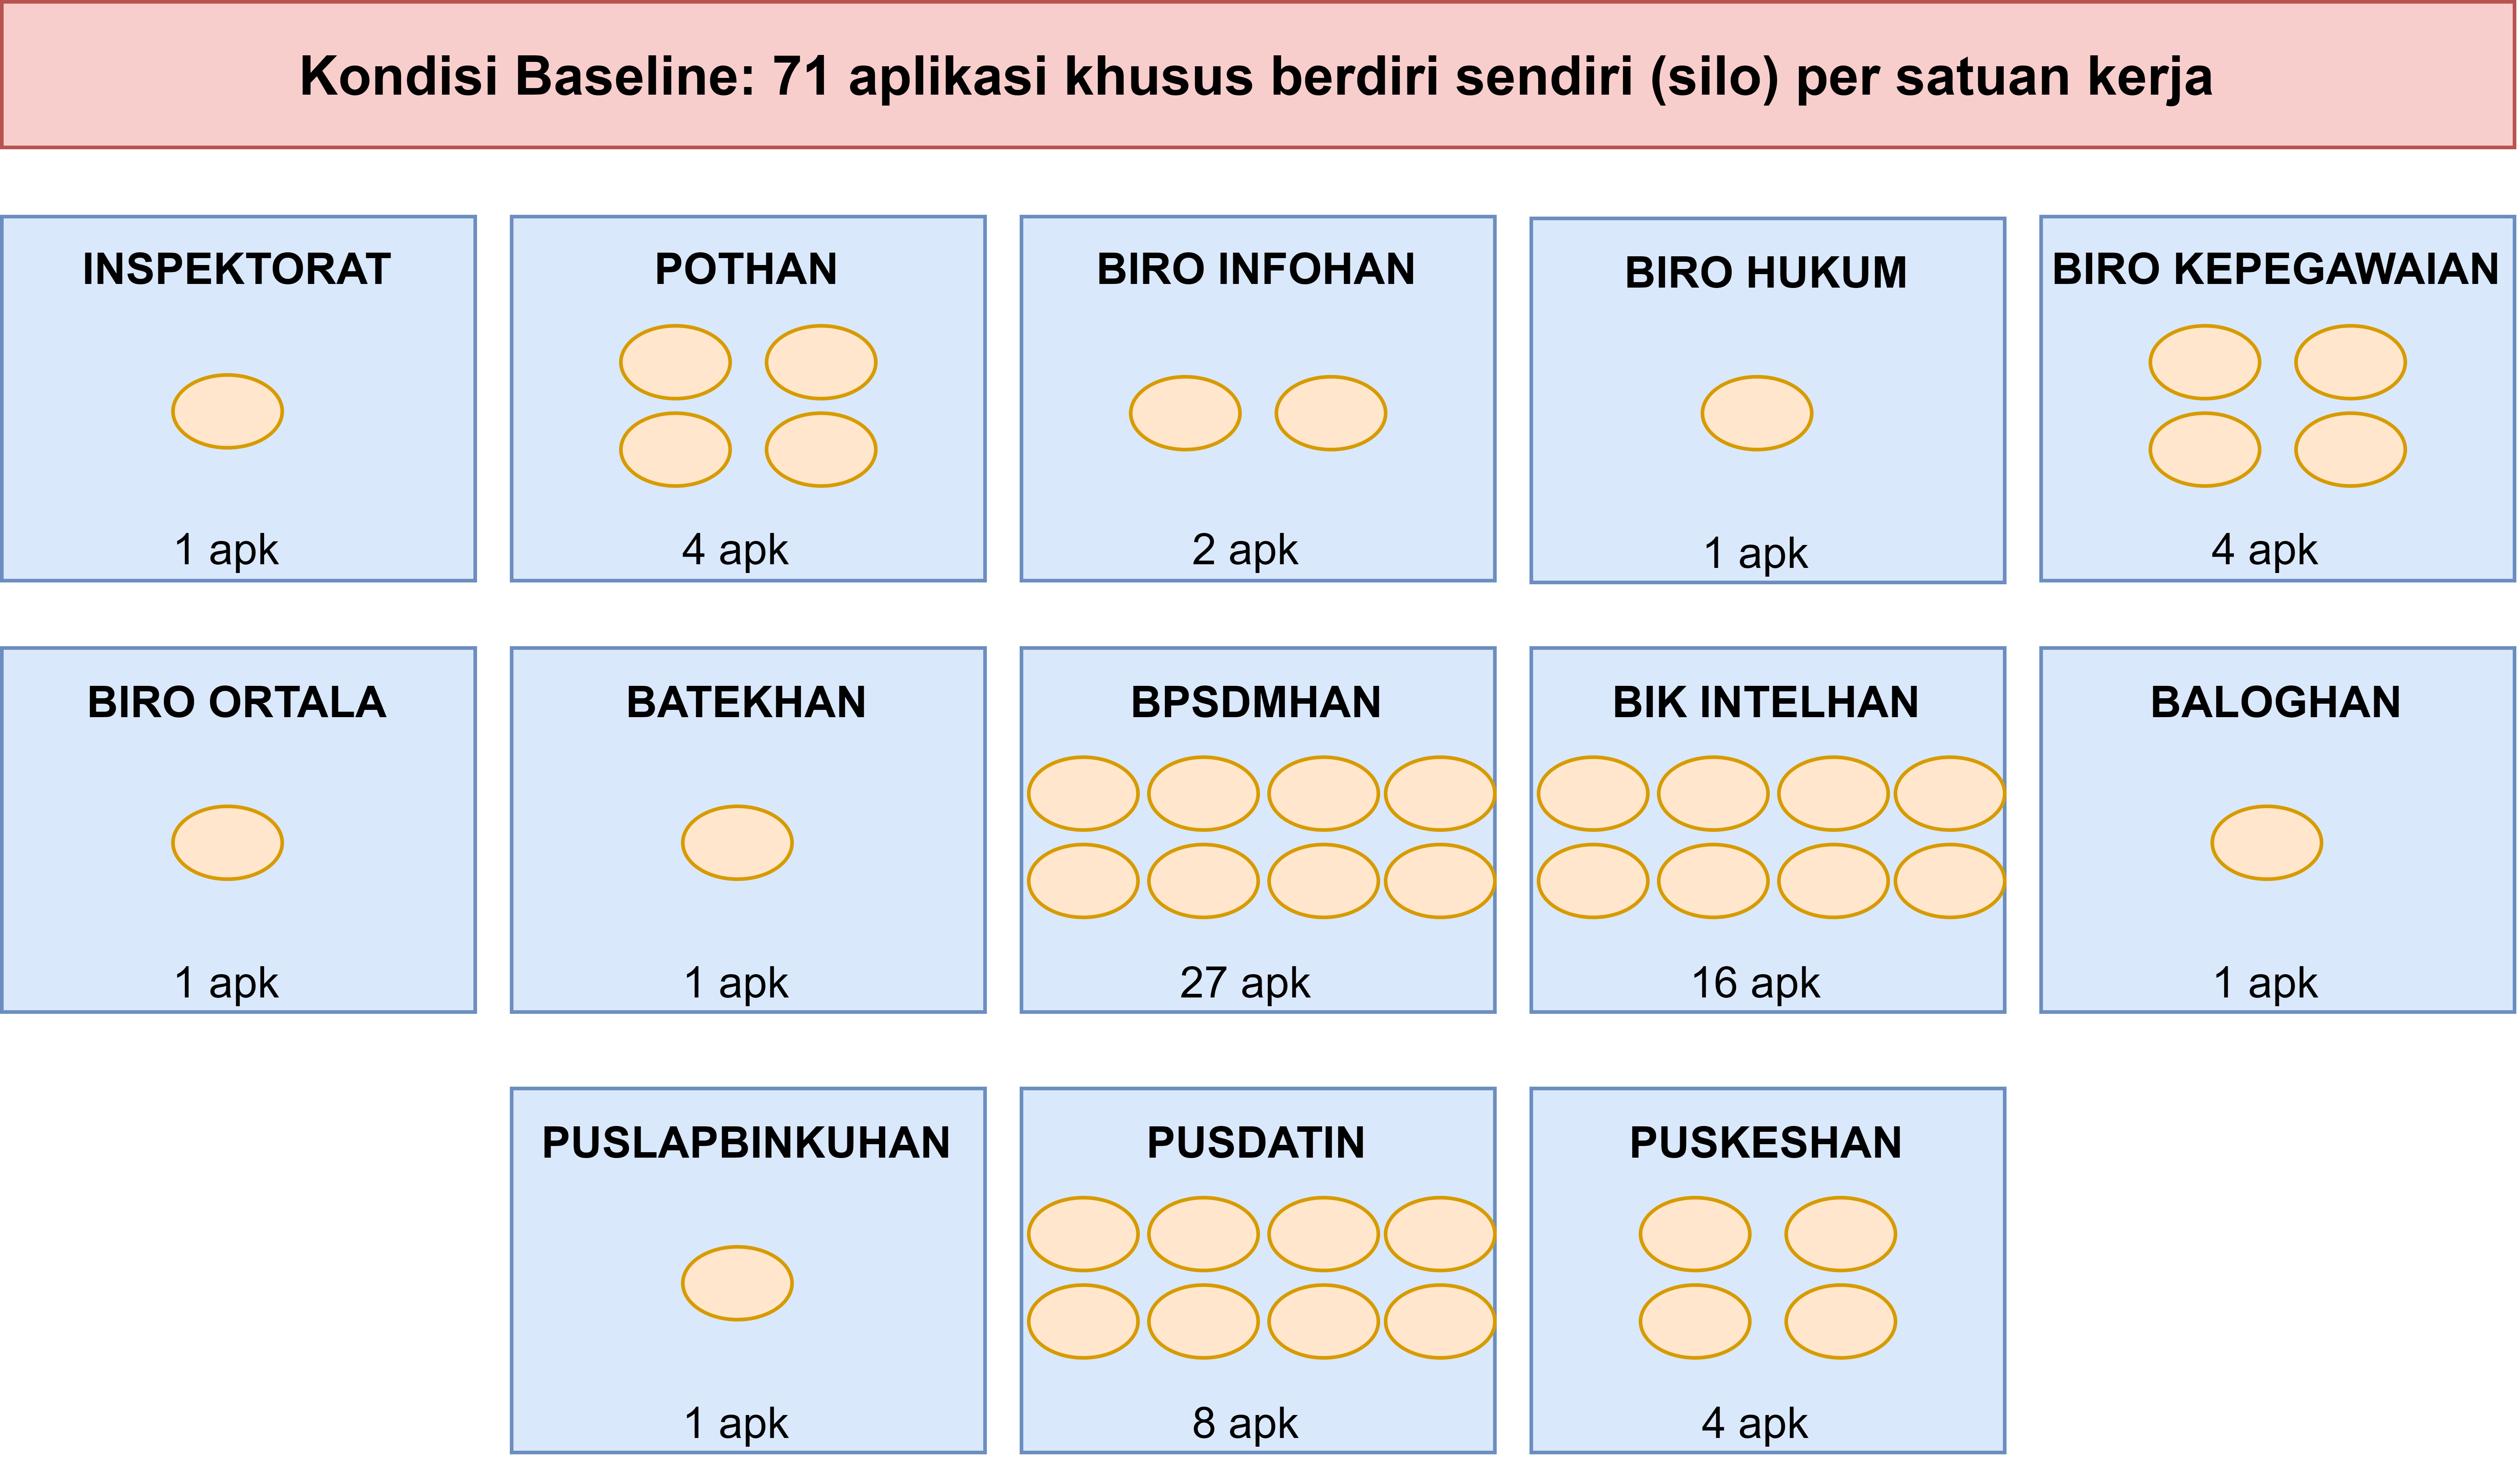
\includegraphics[width=1.00\linewidth,height=0.8\textheight,keepaspectratio]{images/Baseline Integrasi antar Aplikasi (Silo).drawio.png}
\caption{Aplikasi \textit{Baseline}}
\label{fig:IV.10}
\end{figure}

Gambar~\ref{fig:IV.10} menunjukkan bahwa pertukaran data antaraplikasi masih dilakukan secara manual atau terbatas. Kondisi ini menimbulkan duplikasi pemasukan data, akun terpisah untuk setiap aplikasi, dan sulitnya menyajikan data terpadu bagi pimpinan. Aplikasi tersebut dikelompokkan ke dalam sepuluh kelompok fungsi, dipetakan ke kategori ARA, dan dirasionalisasi, sebagaimana disajikan pada Tabel~\ref{tab:IV.19}.

\begingroup\small\setstretch{1.0}
\begin{longtable}{@{}>{\raggedright\arraybackslash\hspace{0pt}}p{0.229\linewidth}>{\raggedright\arraybackslash\hspace{0pt}}p{0.240\linewidth}>{\raggedright\arraybackslash\hspace{0pt}}p{0.335\linewidth}>{\raggedright\arraybackslash\hspace{0pt}}p{0.103\linewidth}@{}}
\caption{Pemetaan dan Rasionalisasi Aplikasi Khusus}\label{tab:IV.19}\\
\toprule
\textbf{Kelompok Fungsi} & \textbf{Kategori ARA} & \textbf{Keputusan Rasionalisasi} & \textbf{Jumlah}\\
\midrule
\endfirsthead
\multicolumn{4}{@{}l}{\small\itshape \tablename\ \thetable{} (lanjutan)}\\
\toprule
\textbf{Kelompok Fungsi} & \textbf{Kategori ARA} & \textbf{Keputusan Rasionalisasi} & \textbf{Jumlah}\\
\midrule
\endhead
\bottomrule
\endlastfoot
Kepegawaian & Administrasi pertahanan & Digabungkan menjadi layanan kepegawaian terpadu & \centering\arraybackslash 5\\*
Hukum dan pengawasan & Administrasi pertahanan & Dipertahankan dan diintegrasikan & \centering\arraybackslash 2\\
Informasi publik & Administrasi pertahanan & Dipertahankan dan diintegrasikan & \centering\arraybackslash 2\\
Potensi pertahanan & Administrasi pertahanan & Dipertahankan dan diintegrasikan & \centering\arraybackslash 4\\
Sarana pertahanan & Administrasi pertahanan & Dipertahankan dan diintegrasikan & \centering\arraybackslash 1\\
Pendidikan dan pelatihan & Administrasi pertahanan & Digabungkan menjadi platform pembelajaran (LMS\label{sk:LMS}) terpadu & \centering\arraybackslash 27\\
Kesehatan dan rehabilitasi & Administrasi pertahanan & Dipertahankan dan diintegrasikan & \centering\arraybackslash 4\\
Data strategis dan geospasial & Aplikasi bersama & Dipertahankan sebagai sumber Portal Satu Data Pertahanan & \centering\arraybackslash 8\\
Keamanan siber dan infrastruktur TIK & Aplikasi bersama dan layanan teknologi & Dipertahankan; pemantauannya dipadukan dalam pusat operasi keamanan & \centering\arraybackslash 16\\*
Litbang dan keuangan & Administrasi pertahanan & Dipertahankan dan diintegrasikan & \centering\arraybackslash 2\\
\end{longtable}
\endgroup

Tabel~\ref{tab:IV.19} menunjukkan bahwa 32 aplikasi pada kelompok kepegawaian serta pendidikan dan pelatihan digabungkan menjadi dua layanan terpadu, sedangkan 39 aplikasi lainnya dipertahankan dan dihubungkan ke platform integrasi. Pemetaan ke ARA juga menunjukkan bahwa belum ada aplikasi pada kategori layanan integrasi dan aplikasi operasional C6ISR.

\subsubsection{Arsitektur Aplikasi Target}
\label{sec:IV.5.2.2}

Arsitektur aplikasi target terdiri atas aplikasi hasil rasionalisasi dan komponen baru yang menutup kategori ARA yang kosong. Komponen baru dirancang sebagai perwujudan ABB DERA, sebagaimana disajikan pada Tabel~\ref{tab:IV.20}.

\begingroup\small\setstretch{1.0}
\begin{longtable}{@{}>{\raggedright\arraybackslash\hspace{0pt}}p{0.418\linewidth}>{\raggedright\arraybackslash\hspace{0pt}}p{0.302\linewidth}>{\raggedright\arraybackslash\hspace{0pt}}p{0.218\linewidth}@{}}
\caption{Komponen Aplikasi Target dan ABB DERA}\label{tab:IV.20}\\
\toprule
\textbf{Komponen Aplikasi Target} & \textbf{Kategori ARA} & \textbf{ABB DERA}\\
\midrule
\endfirsthead
\multicolumn{3}{@{}l}{\small\itshape \tablename\ \thetable{} (lanjutan)}\\
\toprule
\textbf{Komponen Aplikasi Target} & \textbf{Kategori ARA} & \textbf{ABB DERA}\\
\midrule
\endhead
\bottomrule
\endlastfoot
Platform Integrasi Pertahanan (API \textit{gateway} dan pertukaran data) & Layanan integrasi & ABB-02\\*
Portal Satu Data Pertahanan & Aplikasi bersama & ABB-03\\
Layanan SSO/IAM\label{sk:IAM} tingkat \textit{enterprise} & Aplikasi bersama & ABB-01\\
Dasbor eksekutif dan analitik & Aplikasi bersama & ABB-07\\
Tampilan Pemantauan Terpusat (TPT\label{sk:TPT}) tingkat strategis & Aplikasi operasional C6ISR & ABB-04\\*
Layanan kepegawaian dan LMS terpadu & Administrasi pertahanan & \centering\arraybackslash –\\
\end{longtable}
\endgroup

Tabel~\ref{tab:IV.20} menunjukkan bahwa lima komponen baru merupakan perwujudan ABB DERA. TPT tingkat strategis menyajikan gambaran situasi bersama bagi pimpinan Kemhan RI sesuai hak aksesnya dan dikembangkan bersama Mabes TNI pada domain operasional terklasifikasi. ABB-05 dan ABB-06 tidak digunakan karena fusi data sensor dan antarmuka dengan sistem tempur berada pada lingkup Mabes TNI. Model integrasi aplikasi target ditunjukkan pada Gambar~\ref{fig:IV.11}.

\begin{figure}[htbp]
\centering
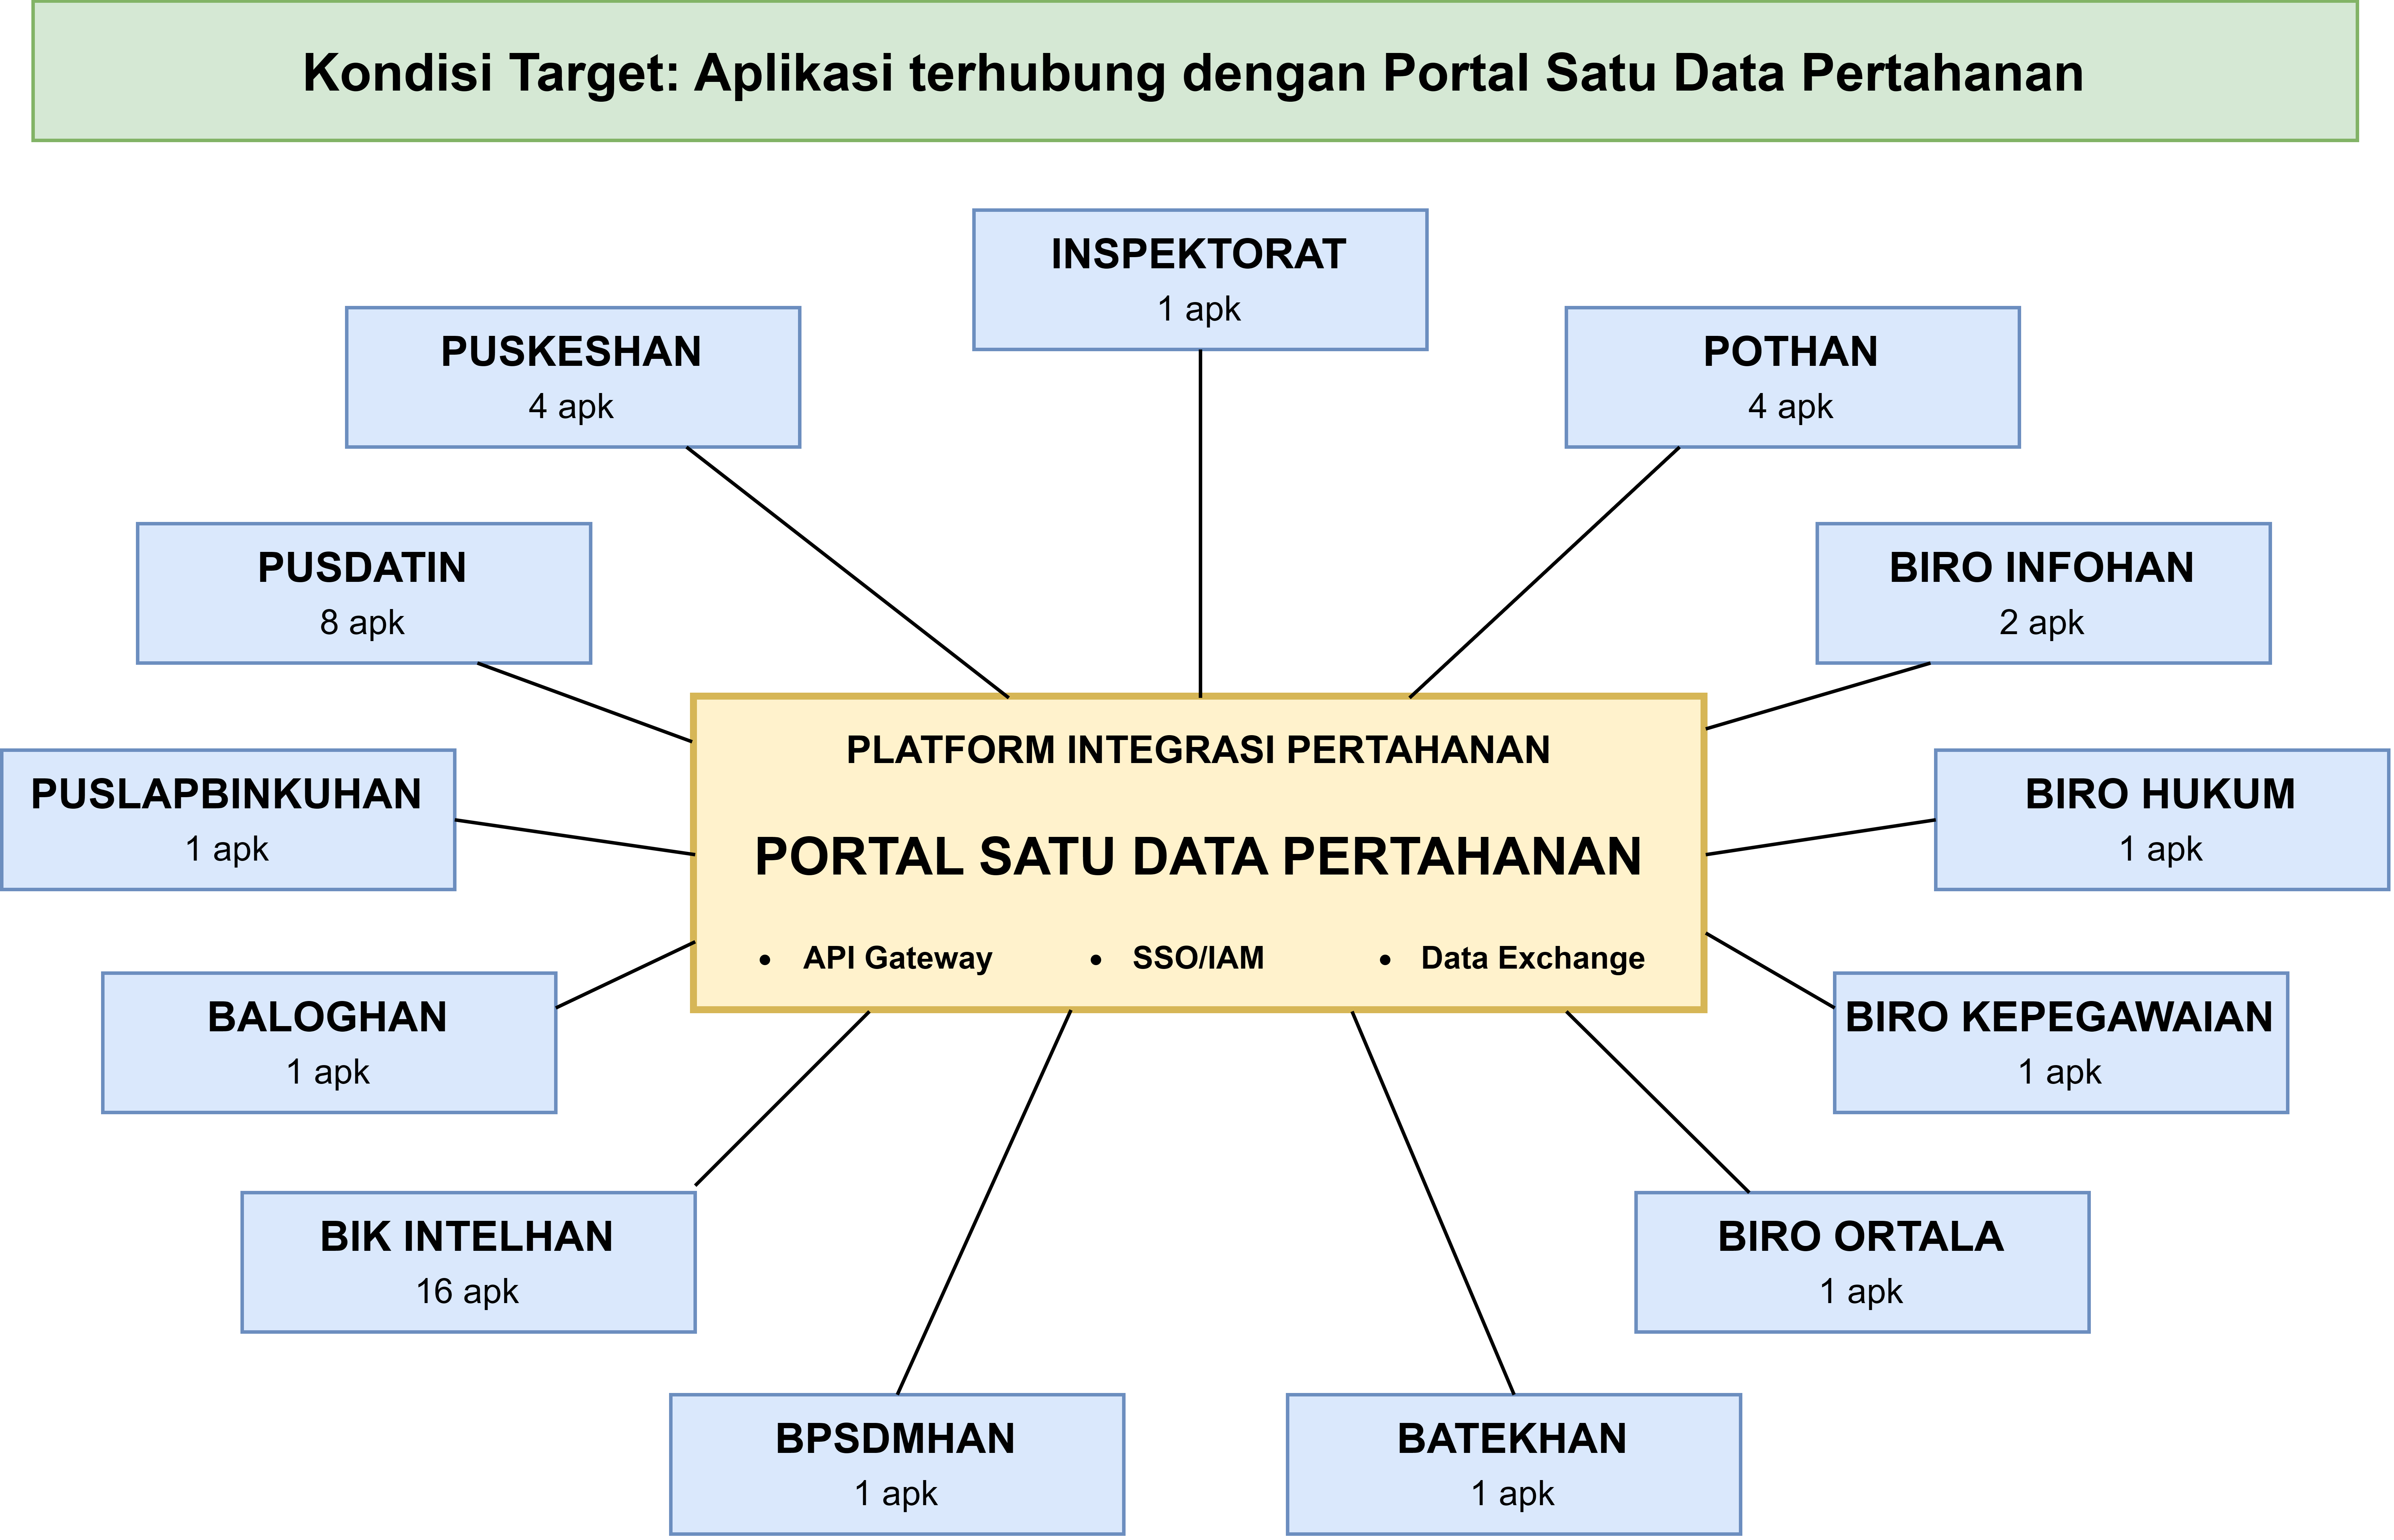
\includegraphics[width=1.00\linewidth,height=0.8\textheight,keepaspectratio]{images/Model Integrasi Target dengan Rasionalisasi Aplikasi.drawio.png}
\caption{Model Integrasi Aplikasi Target}
\label{fig:IV.11}
\end{figure}

Gambar~\ref{fig:IV.11} menunjukkan model \textit{hub} yang menggantikan pola \textit{silo} pada Gambar~\ref{fig:IV.10}. Pertukaran data dilakukan melalui API \textit{gateway} dan pertukaran data dengan otentikasi tunggal, serta dikendalikan sesuai klasifikasi pada Tabel~\ref{tab:IV.16}. Setiap aplikasi cukup terhubung ke satu platform, sehingga integrasi lebih sederhana, aman, dan mudah dikelola. Perluasan SSO ke seluruh aplikasi melanjutkan inisiatif yang telah dirintis Pusat Data dan Informasi.

\subsubsection{Analisis Kesenjangan Aplikasi}
\label{sec:IV.5.2.3}

Analisis kesenjangan arsitektur aplikasi disajikan pada Tabel~\ref{tab:IV.21}.

\begingroup\small\setstretch{1.0}
\begin{longtable}{@{}>{\raggedright\arraybackslash\hspace{0pt}}p{0.066\linewidth}>{\raggedright\arraybackslash\hspace{0pt}}p{0.177\linewidth}>{\raggedright\arraybackslash\hspace{0pt}}p{0.210\linewidth}>{\raggedright\arraybackslash\hspace{0pt}}p{0.213\linewidth}>{\raggedright\arraybackslash\hspace{0pt}}p{0.210\linewidth}@{}}
\caption{Analisis Kesenjangan Arsitektur Aplikasi}\label{tab:IV.21}\\
\toprule
\textbf{No.} & \textbf{Aspek} & \textbf{Kondisi \textit{Baseline}} & \textbf{Kondisi Target} & \textbf{Tindak Lanjut}\\
\midrule
\endfirsthead
\multicolumn{5}{@{}l}{\small\itshape \tablename\ \thetable{} (lanjutan)}\\
\toprule
\textbf{No.} & \textbf{Aspek} & \textbf{Kondisi \textit{Baseline}} & \textbf{Kondisi Target} & \textbf{Tindak Lanjut}\\
\midrule
\endhead
\bottomrule
\endlastfoot
\centering\arraybackslash 1 & Integrasi antaraplikasi & Aplikasi \textit{silo}; pertukaran data manual & Aplikasi terhubung melalui platform integrasi & Pembangunan platform integrasi dan API \textit{gateway}\\*
\centering\arraybackslash 2 & Redundansi fungsi & Aplikasi berfungsi serupa pada kepegawaian dan pembelajaran & Portofolio ramping dan terkonsolidasi & Penggabungan menjadi layanan kepegawaian dan LMS terpadu\\
\centering\arraybackslash 3 & Otentikasi dan akses & Akun terpisah per aplikasi; SSO belum mencakup seluruh aplikasi & SSO/IAM tingkat \textit{enterprise} & Perluasan SSO/IAM ke seluruh aplikasi\\
\centering\arraybackslash 4 & Dukungan C6ISR & Belum ada aplikasi operasional C6ISR maupun dasbor pimpinan terpadu & TPT tingkat strategis serta dasbor eksekutif dan analitik & Pengembangan TPT bersama Mabes TNI serta dasbor eksekutif\\*
\centering\arraybackslash 5 & Tata kelola aplikasi & Pengelolaan aplikasi tersebar per satuan kerja & Tata kelola portofolio aplikasi terpusat & Penetapan tata kelola portofolio aplikasi oleh DTO\\
\end{longtable}
\endgroup

Tabel~\ref{tab:IV.21} menunjukkan bahwa platform integrasi menjadi prasyarat bagi penutupan kesenjangan lainnya.

\section{Fase D: Technology Architecture}
\label{sec:IV.6}

Fase \textit{Technology Architecture} merancang infrastruktur teknologi yang menopang arsitektur data dan aplikasi. Pada langkah \textit{Select Reference Models, Viewpoints, and Tools}, TRA dan posisi teknis DERA dipilih sebagai acuan, sedangkan aspek keamanan mengacu pada Permenhan Nomor 34 Tahun 2025 \cite{Permenhan34Tahun2025}.

\subsection{Arsitektur Teknologi Baseline}
\label{sec:IV.6.1}

Topologi jaringan dan infrastruktur pusat data Kemhan RI secara rinci tidak tersedia dalam penelitian ini. Oleh karena itu, arsitektur teknologi \textit{baseline} disusun sebagai model logis berdasarkan informasi yang tersedia, sebagaimana disajikan pada Gambar~\ref{fig:IV.12}.

\begin{figure}[htbp]
\centering
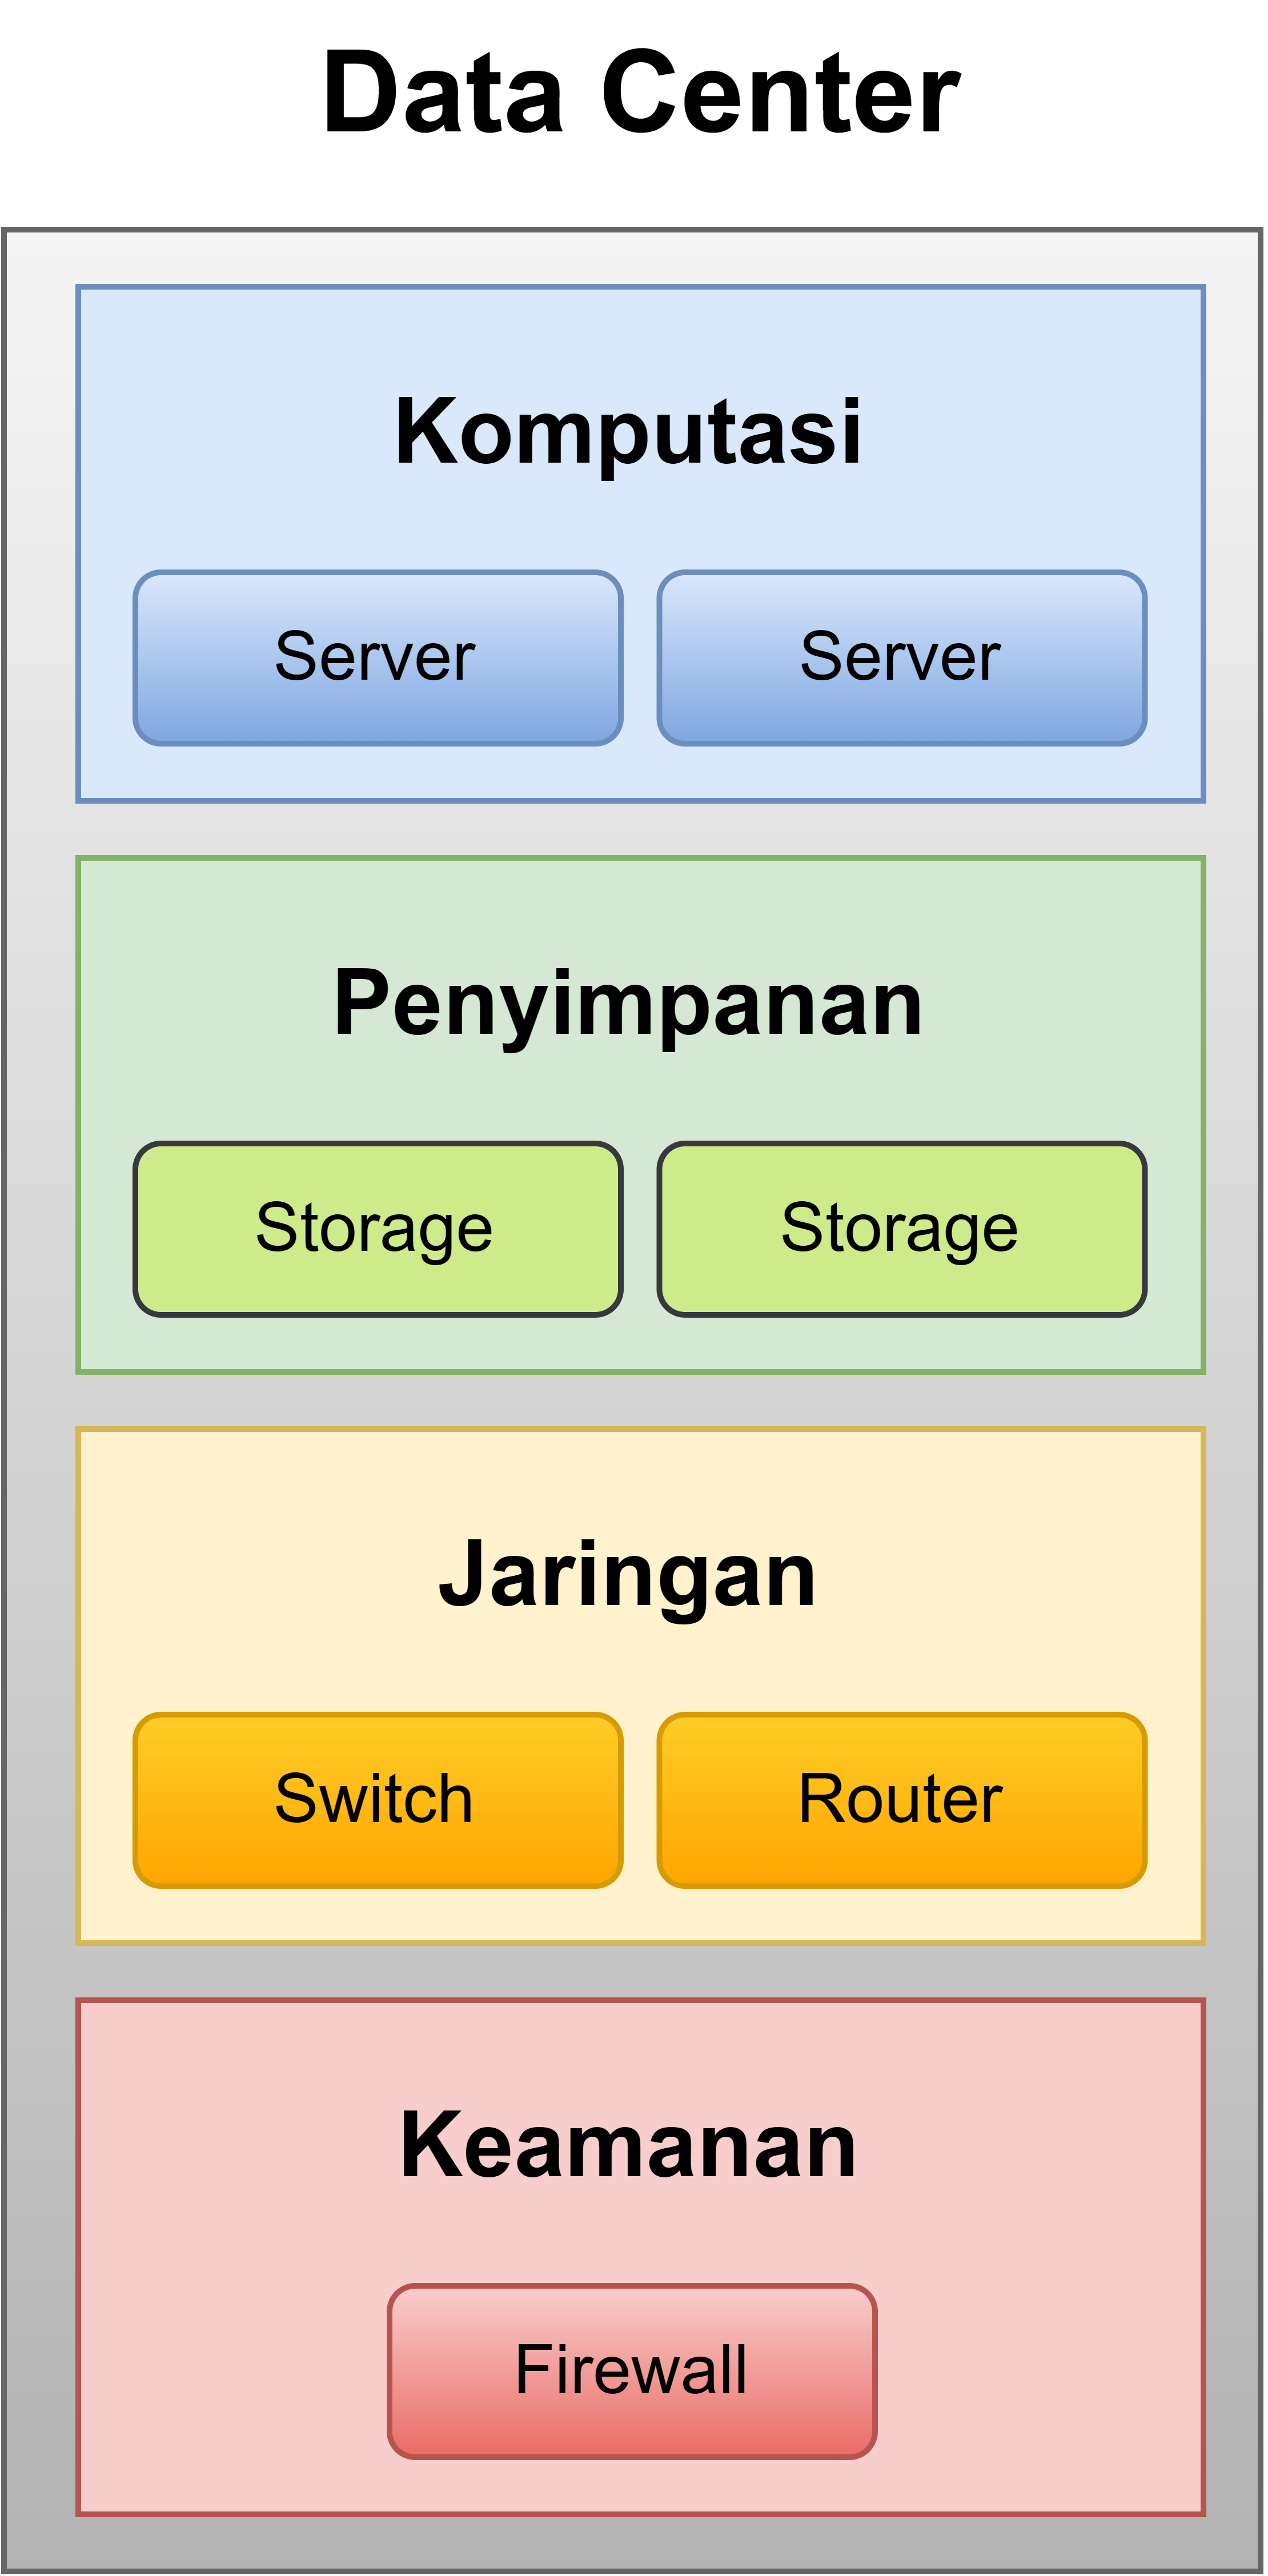
\includegraphics[width=0.33\linewidth,height=0.8\textheight,keepaspectratio]{images/Arsitektur Teknologi Baseline.drawio.png}
\caption{Arsitektur Teknologi \textit{Baseline}}
\label{fig:IV.12}
\end{figure}

Gambar~\ref{fig:IV.12} menunjukkan bahwa infrastruktur teknologi Kemhan RI berpusat pada satu pusat data di Pusat Data dan Informasi, Pondok Labu, Jakarta Selatan. Infrastruktur tersebut terdiri atas lapisan komputasi, penyimpanan, jaringan, dan keamanan. Terdapat dua karakteristik utama. Pertama, seluruh layanan bertumpu pada satu pusat data tanpa pusat pemulihan bencana, sehingga menjadi titik tunggal kegagalan. Kedua, keamanan masih bersifat parsial dan belum ada jaringan operasional terklasifikasi yang terpisah.

\subsection{Prinsip dan Standar Teknologi}
\label{sec:IV.6.2}

Penerapan prinsip DERA pada domain teknologi disajikan pada Tabel~\ref{tab:IV.22}.

\begingroup\small\setstretch{1.0}
\begin{longtable}{@{}>{\raggedright\arraybackslash\hspace{0pt}}p{0.281\linewidth}>{\raggedright\arraybackslash\hspace{0pt}}p{0.688\linewidth}@{}}
\caption{Penerapan Prinsip DERA pada Arsitektur Teknologi}\label{tab:IV.22}\\
\toprule
\textbf{Prinsip} & \textbf{Penerapan pada Arsitektur Teknologi}\\
\midrule
\endfirsthead
\multicolumn{2}{@{}l}{\small\itshape \tablename\ \thetable{} (lanjutan)}\\
\toprule
\textbf{Prinsip} & \textbf{Penerapan pada Arsitektur Teknologi}\\
\midrule
\endhead
\bottomrule
\endlastfoot
\textit{Availability \& Reliability} & Pusat data dilengkapi pusat pemulihan bencana, redundansi, dan cadangan untuk menjamin ketersediaan layanan\\*
\textit{Security by Design} & Keamanan diterapkan sejak perancangan pada setiap lapisan, termasuk pemisahan domain klasifikasi\\
\textit{Scalability \& Flexibility} & Virtualisasi dan kontainer agar sumber daya elastis dan mudah diskalakan\\
\textit{Interoperability} & Standar terbuka dan API untuk pertukaran data antarsistem\\
\textit{Integrated Command \& Control} & Jaringan operasional terklasifikasi yang terhubung dengan Mabes TNI dan matra\\*
\textit{Data as Strategic Asset} & Penyimpanan redundan dan cadangan terpusat untuk melindungi Data Pertahanan\\
\end{longtable}
\endgroup

Tabel~\ref{tab:IV.22} menunjukkan bahwa enam dari sembilan prinsip DERA diterapkan langsung pada domain teknologi. Selain prinsip, arsitektur teknologi mengadopsi posisi teknis DERA (Tabel~\ref{tab:III.19}), yaitu ISO/IEC 27001 \cite{ISO27001}, Pedoman Pertahanan Siber \cite{Permenhan82Tahun2014}, dan Arsitektur SPBE Nasional \cite{Perpres132Tahun2022}, ditambah ketentuan telekomunikasi khusus pertahanan \cite{Permenhan8Tahun2016} sebagai standar internal Kemhan RI.

\subsection{Arsitektur Teknologi Target}
\label{sec:IV.6.3}

Arsitektur teknologi target dirancang untuk menutup kesenjangan \textit{baseline} serta menopang Platform Integrasi Pertahanan, Portal Satu Data Pertahanan, dan TPT tingkat strategis. Arsitektur ini menerapkan pola P3, P4, dan P5, sebagaimana ditunjukkan pada Gambar~\ref{fig:IV.13}.

\begin{figure}[htbp]
\centering
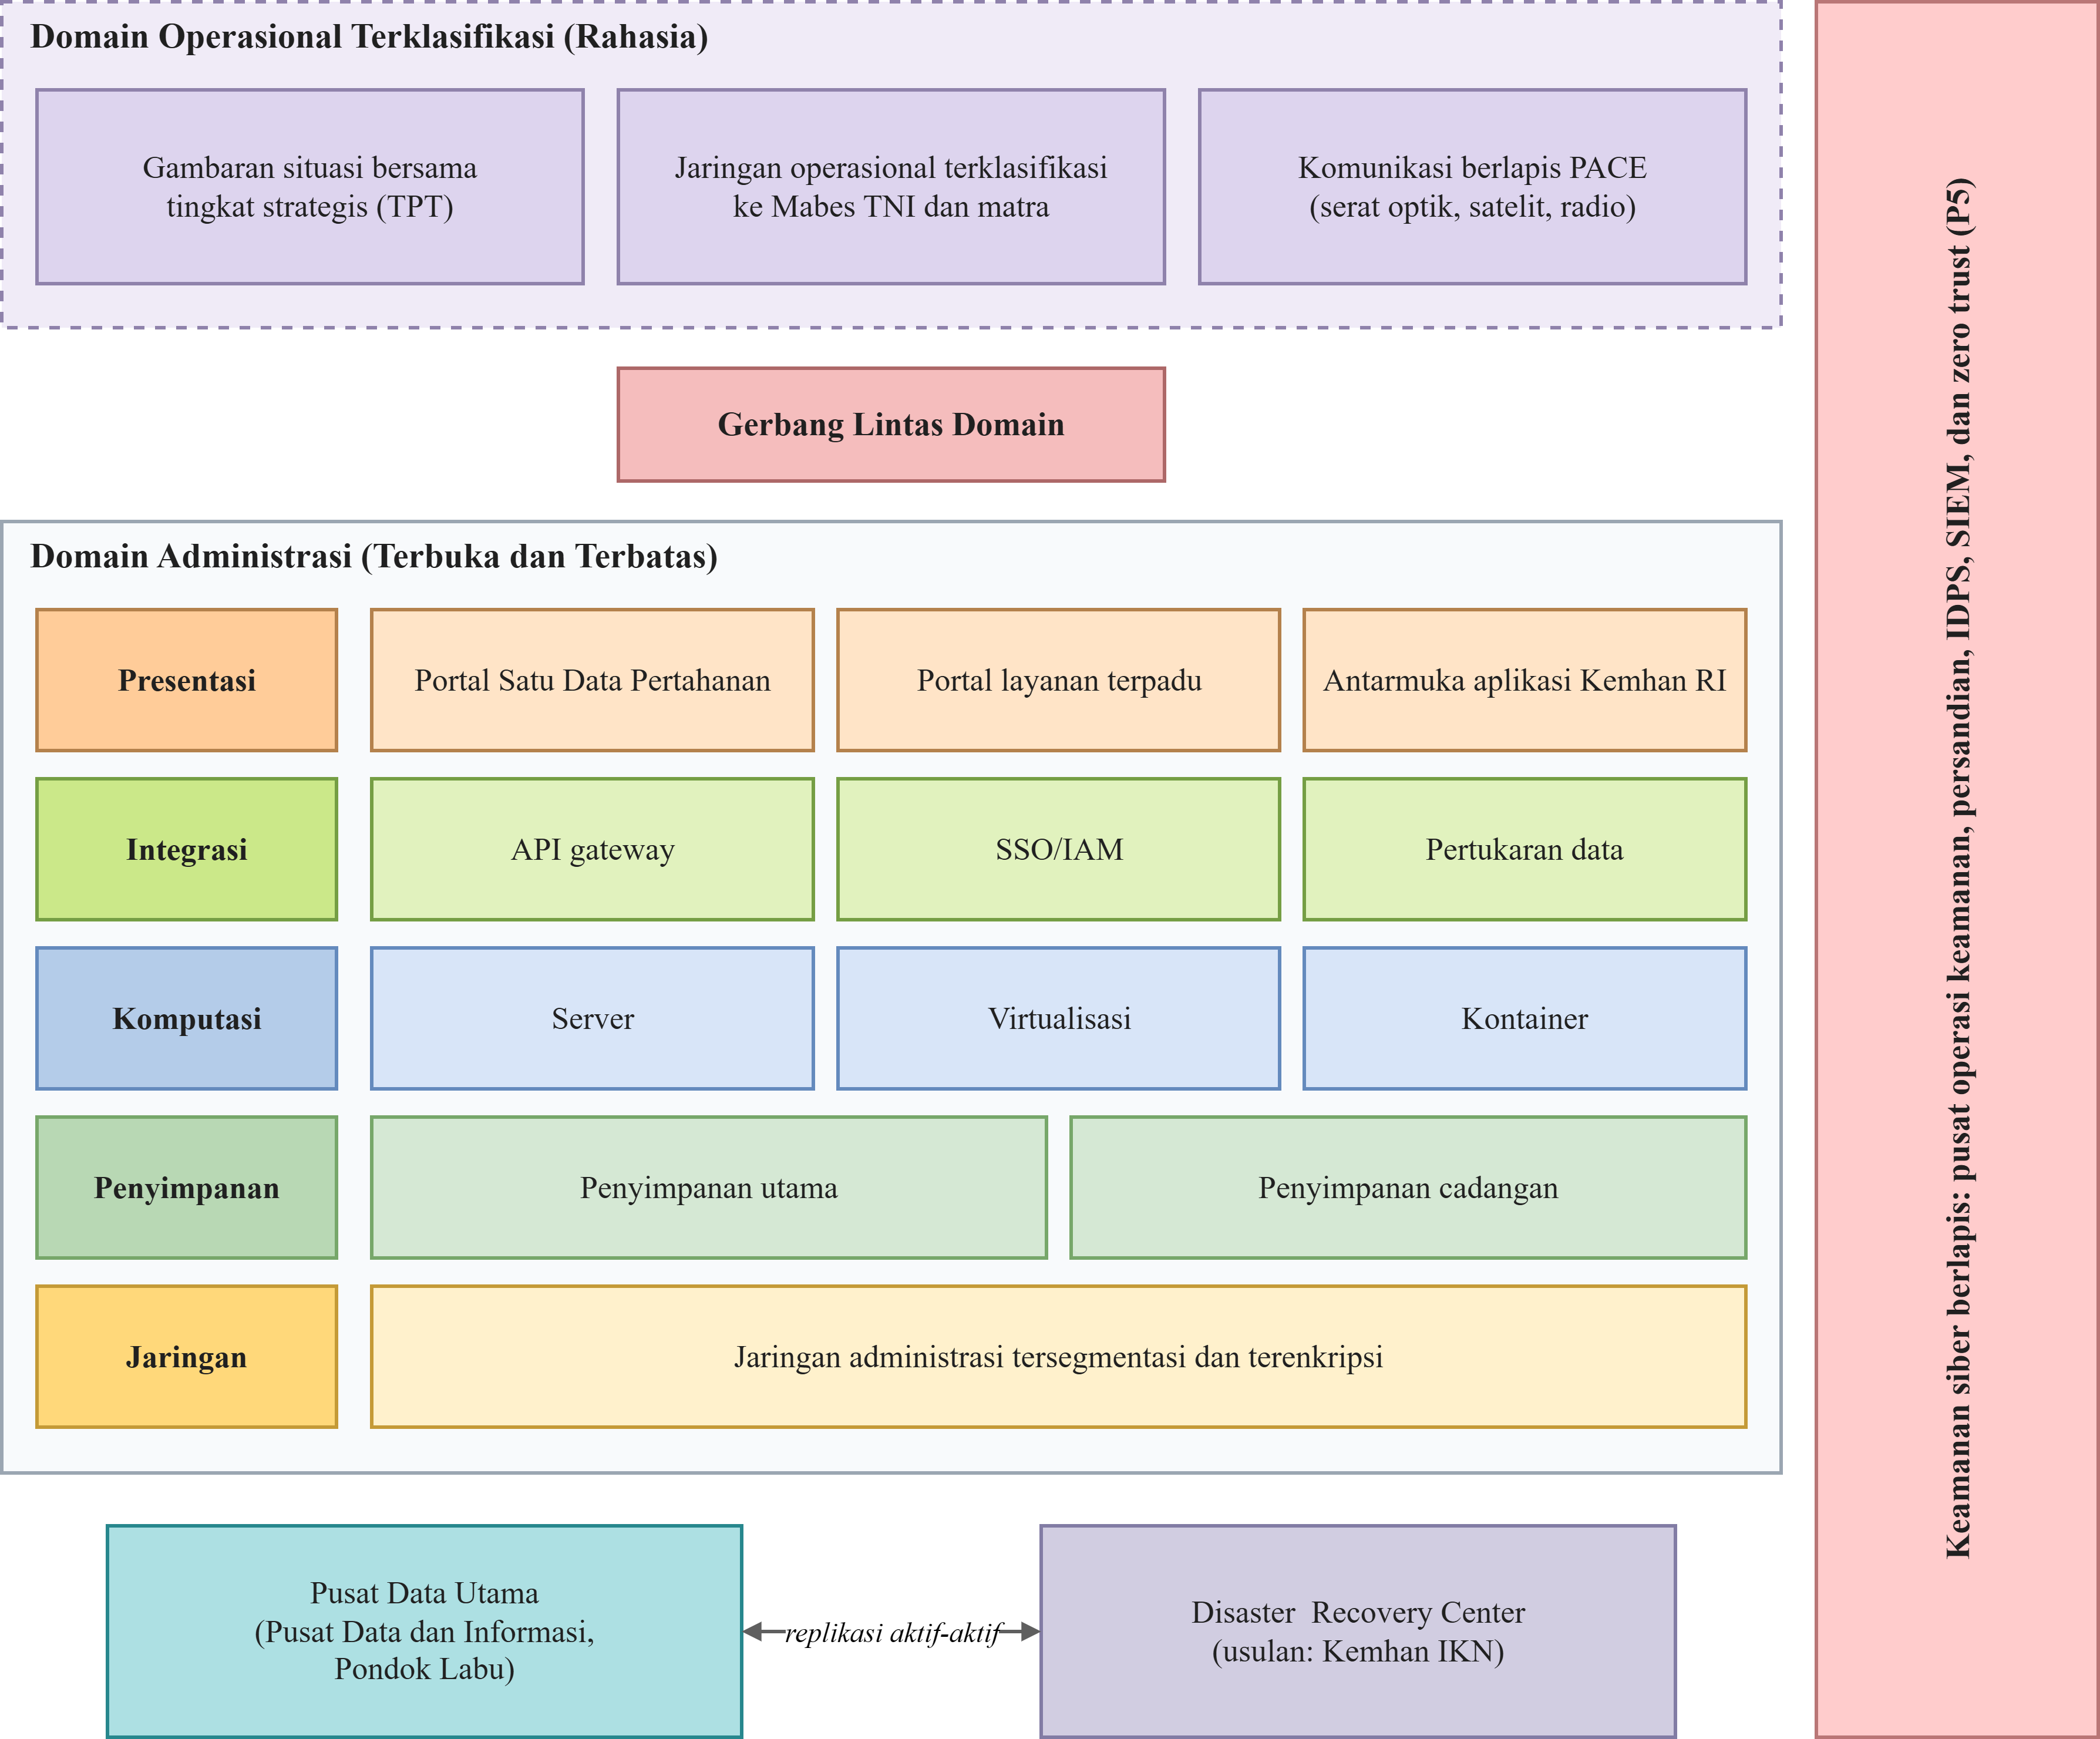
\includegraphics[width=1.00\linewidth,height=0.8\textheight,keepaspectratio]{images/Gambar_IV.13_Arsitektur_Teknologi_Target_Berwarna.drawio.png}
\caption{Arsitektur Teknologi Target}
\label{fig:IV.13}
\end{figure}

Gambar~\ref{fig:IV.13} menunjukkan bahwa arsitektur teknologi target terdiri atas komponen berikut.

\begin{enumerate}[label=\arabic*.]
\item Domain administrasi, yang terdiri atas lapisan presentasi, integrasi, komputasi, penyimpanan, dan jaringan administrasi yang tersegmentasi dan terenkripsi.
\item Domain operasional terklasifikasi (ABB-11), yang menghubungkan TPT tingkat strategis dengan Mabes TNI dan matra melalui komunikasi berlapis PACE (ABB-10).
\item Gerbang lintas domain (ABB-11), yang mengendalikan pertukaran data antara kedua domain sesuai pola P5.
\item Pusat data utama di Pusat Data dan Informasi, Pondok Labu, dan pusat pemulihan bencana yang diusulkan berlokasi di Kemhan IKN\label{sk:IKN} (ABB-08). Keduanya beroperasi aktif-aktif dengan replikasi data, sehingga titik tunggal kegagalan dapat dihilangkan.
\item Keamanan siber berlapis yang membentang pada kedua domain, dengan pusat operasi keamanan (ABB-12) sebagai pusat pemantauan.
\end{enumerate}

Komputasi \textit{edge} (ABB-09) tidak diterapkan pada Kemhan RI karena digunakan pada tingkat platform dan satuan di bawah Mabes TNI.

\subsection{Arsitektur Keamanan}
\label{sec:IV.6.4}

Arsitektur keamanan mengacu pada Permenhan Nomor 34 Tahun 2025 \cite{Permenhan34Tahun2025}, yang mengelompokkan pelindungan ke dalam empat domain, yaitu identifikasi, proteksi, deteksi, serta penanggulangan dan pemulihan. Komponen keamanan pada setiap domain disajikan pada Tabel~\ref{tab:IV.23}.

\begingroup\small\setstretch{1.0}
\begin{longtable}{@{}>{\raggedright\arraybackslash\hspace{0pt}}p{0.201\linewidth}>{\raggedright\arraybackslash\hspace{0pt}}p{0.441\linewidth}>{\raggedright\arraybackslash\hspace{0pt}}p{0.296\linewidth}@{}}
\caption{Komponen Keamanan per Domain}\label{tab:IV.23}\\
\toprule
\textbf{Domain} & \textbf{Komponen} & \textbf{Fungsi}\\
\midrule
\endfirsthead
\multicolumn{3}{@{}l}{\small\itshape \tablename\ \thetable{} (lanjutan)}\\
\toprule
\textbf{Domain} & \textbf{Komponen} & \textbf{Fungsi}\\
\midrule
\endhead
\bottomrule
\endlastfoot
Identifikasi & \textit{Vulnerability Assessment and Penetration Test} (VAPT\label{sk:VAPT}) & Mengidentifikasi kerentanan dan risiko keamanan sistem\\*
Proteksi & \textit{Firewall}, segmentasi jaringan, pemisahan domain klasifikasi, gerbang lintas domain, persandian, \textit{endpoint protection}, dan IDPS\label{sk:IDPS} & Melindungi jaringan, data, dan perangkat serta mencegah serangan\\
Deteksi & \textit{Cyber Threat Intelligence} (CTI\label{sk:CTI}) dan SIEM\label{sk:SIEM} pada pusat operasi keamanan & Mendeteksi anomali dan peristiwa keamanan siber\\*
Penanggulangan dan pemulihan & \textit{Digital forensic}, SOAR\label{sk:SOAR}, CSIRT\label{sk:CSIRT}, sistem cadangan, dan pusat pemulihan bencana & Menanggulangi insiden siber serta memulihkan layanan\\
\end{longtable}
\endgroup

Tabel~\ref{tab:IV.23} menunjukkan bahwa sebagian komponen telah tersedia pada kondisi \textit{baseline}, seperti VAPT, SIEM, dan \textit{Helpdesk} CSIRT. Oleh karena itu, arah pengembangannya adalah memadukan komponen tersebut dalam satu pusat operasi keamanan. Sesuai peta jalan tersebut, kematangan keamanan siber sektor pertahanan saat ini berada pada level 1 hingga level 2, dengan target level 3 pada tahun 2029 \cite{Permenhan34Tahun2025}.

\subsection{Analisis Kesenjangan}
\label{sec:IV.6.5}

Analisis kesenjangan arsitektur teknologi disajikan pada Tabel~\ref{tab:IV.24}.

\begingroup\small\setstretch{1.0}
\begin{longtable}{@{}>{\raggedright\arraybackslash\hspace{0pt}}p{0.066\linewidth}>{\raggedright\arraybackslash\hspace{0pt}}p{0.177\linewidth}>{\raggedright\arraybackslash\hspace{0pt}}p{0.210\linewidth}>{\raggedright\arraybackslash\hspace{0pt}}p{0.213\linewidth}>{\raggedright\arraybackslash\hspace{0pt}}p{0.210\linewidth}@{}}
\caption{Analisis Kesenjangan Arsitektur Teknologi}\label{tab:IV.24}\\
\toprule
\textbf{No.} & \textbf{Aspek} & \textbf{Kondisi \textit{Baseline}} & \textbf{Kondisi Target} & \textbf{Tindak Lanjut}\\
\midrule
\endfirsthead
\multicolumn{5}{@{}l}{\small\itshape \tablename\ \thetable{} (lanjutan)}\\
\toprule
\textbf{No.} & \textbf{Aspek} & \textbf{Kondisi \textit{Baseline}} & \textbf{Kondisi Target} & \textbf{Tindak Lanjut}\\
\midrule
\endhead
\bottomrule
\endlastfoot
\centering\arraybackslash 1 & Ketersediaan & Satu pusat data tanpa pusat pemulihan bencana & Pusat data utama dan pusat pemulihan bencana aktif-aktif & Pembangunan pusat pemulihan bencana dan replikasi aktif-aktif\\*
\centering\arraybackslash 2 & Komputasi & Server fisik & Server, virtualisasi, dan kontainer & Penerapan virtualisasi dan kontainer\\
\centering\arraybackslash 3 & Penyimpanan & Penyimpanan tanpa redundansi & Penyimpanan utama dan cadangan yang redundan & Penyediaan redundansi dan cadangan data\\
\centering\arraybackslash 4 & Jaringan & Belum tersegmentasi dan belum lintas matra & Tersegmentasi, terenkripsi, dan berlapis PACE & Penataan jaringan dan penerapan skema PACE\\
\centering\arraybackslash 5 & Integrasi & Belum ada lapisan integrasi & Lapisan integrasi (API \textit{gateway}, SSO/IAM, dan pertukaran data) & Pembangunan lapisan integrasi\\
\centering\arraybackslash 6 & Domain klasifikasi & Belum ada jaringan operasional terklasifikasi yang terpisah & Domain operasional terklasifikasi dengan gerbang lintas domain & Pembangunan jaringan terklasifikasi dan gerbang lintas domain\\*
\centering\arraybackslash 7 & Keamanan & Parsial (kematangan level 1–2) & Menyeluruh dengan pusat operasi keamanan (kematangan level 3) & Penerapan komponen keamanan per domain\\
\end{longtable}
\endgroup

Tabel~\ref{tab:IV.24} menunjukkan bahwa kesenjangan 1 merupakan risiko terbesar karena gangguan pada satu pusat data dapat menghentikan seluruh layanan pertahanan.

\section{Fase E: Opportunities and Solutions}
\label{sec:IV.7}

Fase \textit{Opportunities and Solutions} menerjemahkan hasil Fase B hingga D menjadi rencana pelaksanaan. Sesuai Tabel~\ref{tab:III.22}, fase ini menggunakan pola lintas domain dan ABB DERA untuk mengelompokkan kesenjangan ke dalam paket pekerjaan, mewujudkan ABB menjadi SBB, serta menyusun arsitektur transisi dan \textit{roadmap} arsitektur.

\subsection{Atribut Perubahan dan Kendala}
\label{sec:IV.7.1}

Atribut perubahan menggambarkan pergeseran kondisi yang ingin dicapai melalui transformasi, sebagaimana disajikan pada Tabel~\ref{tab:IV.25}.

\begingroup\small\setstretch{1.0}
\begin{longtable}{@{}>{\raggedright\arraybackslash\hspace{0pt}}p{0.201\linewidth}>{\raggedright\arraybackslash\hspace{0pt}}p{0.359\linewidth}>{\raggedright\arraybackslash\hspace{0pt}}p{0.378\linewidth}@{}}
\caption{Atribut Perubahan Utama}\label{tab:IV.25}\\
\toprule
\textbf{Atribut} & \textbf{Kondisi Saat Ini} & \textbf{Arah Perubahan}\\
\midrule
\endfirsthead
\multicolumn{3}{@{}l}{\small\itshape \tablename\ \thetable{} (lanjutan)}\\
\toprule
\textbf{Atribut} & \textbf{Kondisi Saat Ini} & \textbf{Arah Perubahan}\\
\midrule
\endhead
\bottomrule
\endlastfoot
Tata kelola transformasi & Berjalan parsial tanpa mandat lintas organisasi & Terorkestrasi oleh DTO dan \textit{Architecture Board} dengan DERA sebagai acuan\\*
Data & Terkotak per aplikasi dan satuan kerja & Satu Data Pertahanan yang terstandar dan terklasifikasi\\
Aplikasi & 71 aplikasi khusus bersifat \textit{silo} dan sebagian berfungsi serupa & Aplikasi terkonsolidasi dan terintegrasi\\
Infrastruktur & Satu pusat data tanpa pusat pemulihan bencana & Pusat data utama dan pusat pemulihan bencana aktif-aktif\\
Keamanan siber & Parsial dengan kematangan level 1–2 & Menyeluruh dengan kematangan level 3 dan pemisahan domain klasifikasi\\*
C6ISR & Belum ada gambaran situasi bersama dengan Mabes TNI & TPT tingkat strategis melalui domain operasional terklasifikasi\\
\end{longtable}
\endgroup

Tabel~\ref{tab:IV.25} menunjukkan bahwa perubahan terjadi serentak pada enam atribut. Oleh karena itu, transformasi perlu ditahapkan dengan memperhatikan kendala pada Tabel~\ref{tab:IV.26}.

\begingroup\small\setstretch{1.0}
\begin{longtable}{@{}>{\raggedright\arraybackslash\hspace{0pt}}p{0.281\linewidth}>{\raggedright\arraybackslash\hspace{0pt}}p{0.688\linewidth}@{}}
\caption{Kendala Implementasi dan Implikasinya}\label{tab:IV.26}\\
\toprule
\textbf{Kendala} & \textbf{Implikasi}\\
\midrule
\endfirsthead
\multicolumn{2}{@{}l}{\small\itshape \tablename\ \thetable{} (lanjutan)}\\
\toprule
\textbf{Kendala} & \textbf{Implikasi}\\
\midrule
\endhead
\bottomrule
\endlastfoot
Keterbatasan SDM digital & Pengembangan talenta digital berjalan paralel dengan paket teknis, sedangkan pelaksanaan awal memanfaatkan unit yang telah ada\\*
Sistem lama (\textit{legacy}) & Integrasi dilakukan bertahap melalui API dan standar terbuka, bukan penggantian sistem sekaligus\\
Kerahasiaan pertahanan & Data Rahasia baru dialirkan setelah domain operasional terklasifikasi dan gerbang lintas domain tersedia\\*
Keterbatasan anggaran dan waktu & Jangka pendek difokuskan pada inisiatif fondasi berbiaya rendah, sedangkan investasi besar ditempatkan pada jangka menengah dan panjang\\
\end{longtable}
\endgroup

Tabel~\ref{tab:IV.26} menunjukkan bahwa setiap kendala membatasi susunan paket pekerjaan dan urutan pelaksanaannya.

\subsection{Konsolidasi Kesenjangan}
\label{sec:IV.7.2}

Kesenjangan dari Fase B hingga D disatukan agar inisiatif yang beririsan tidak dilaksanakan berulang. Hasil konsolidasi disajikan pada Tabel~\ref{tab:IV.27}, dengan kolom asal kesenjangan memuat nomor tabel dan barisnya.

\begingroup\small\setstretch{1.0}
\begin{longtable}{@{}>{\raggedright\arraybackslash\hspace{0pt}}p{0.069\linewidth}>{\raggedright\arraybackslash\hspace{0pt}}p{0.240\linewidth}>{\raggedright\arraybackslash\hspace{0pt}}p{0.370\linewidth}>{\raggedright\arraybackslash\hspace{0pt}}p{0.229\linewidth}@{}}
\caption{Konsolidasi Kesenjangan}\label{tab:IV.27}\\
\toprule
\textbf{No.} & \textbf{Kelompok Kesenjangan} & \textbf{Inti Persoalan} & \textbf{Asal Kesenjangan}\\
\midrule
\endfirsthead
\multicolumn{4}{@{}l}{\small\itshape \tablename\ \thetable{} (lanjutan)}\\
\toprule
\textbf{No.} & \textbf{Kelompok Kesenjangan} & \textbf{Inti Persoalan} & \textbf{Asal Kesenjangan}\\
\midrule
\endhead
\bottomrule
\endlastfoot
\centering\arraybackslash 1 & Tata kelola dan mandat transformasi & Belum ada fungsi yang mengorkestrasi transformasi serta tata kelola arsitektur, data, dan portofolio aplikasi & Tabel~\ref{tab:IV.14} (1, 2); Tabel~\ref{tab:IV.18} (3); Tabel~\ref{tab:IV.21} (5)\\*
\centering\arraybackslash 2 & Proses bisnis, manajemen perubahan, dan talenta digital & Proses terfragmentasi, perubahan tidak dikelola, koordinasi lintas matra \textit{ad hoc}, dan kompetensi digital terbatas & Tabel~\ref{tab:IV.14} (3–6)\\
\centering\arraybackslash 3 & Standar dan berbagi-pakai data & Data terkotak tanpa standar, klasifikasi, dan kanal berbagi-pakai & Tabel~\ref{tab:IV.18} (1, 2, 4, 6)\\
\centering\arraybackslash 4 & Integrasi dan portofolio aplikasi & Aplikasi berdiri sendiri dan sebagian berfungsi serupa, akun terpisah, serta belum ada lapisan integrasi & Tabel~\ref{tab:IV.21} (1–3); Tabel~\ref{tab:IV.24} (5)\\
\centering\arraybackslash 5 & Infrastruktur pusat data dan jaringan & Satu pusat data tanpa pusat pemulihan bencana, server fisik, serta jaringan belum tersegmentasi dan belum berlapis & Tabel~\ref{tab:IV.24} (1–4)\\
\centering\arraybackslash 6 & Keamanan siber dan domain klasifikasi & Pelindungan parsial dan belum ada jaringan operasional terklasifikasi & Tabel~\ref{tab:IV.18} (5); Tabel~\ref{tab:IV.24} (6, 7)\\*
\centering\arraybackslash 7 & Dukungan C6ISR & Belum ada gambaran situasi bersama, pertukaran data situasi, maupun aplikasi operasional C6ISR bersama Mabes TNI & Tabel~\ref{tab:IV.14} (7); Tabel~\ref{tab:IV.18} (7); Tabel~\ref{tab:IV.21} (4)\\
\end{longtable}
\endgroup

Tabel~\ref{tab:IV.27} menunjukkan bahwa 26 kesenjangan dari tiga fase mengerucut menjadi tujuh kelompok. Penggabungan ini mencegah inisiatif yang sama dianggarkan dan dilaksanakan lebih dari satu kali.

\subsection{Paket Pekerjaan}
\label{sec:IV.7.3}

Ketujuh kelompok kesenjangan ditetapkan menjadi tujuh paket pekerjaan, sebagaimana disajikan pada Tabel~\ref{tab:IV.28}.

\begingroup\small\setstretch{1.0}
\begin{longtable}{@{}>{\raggedright\arraybackslash\hspace{0pt}}p{0.103\linewidth}>{\raggedright\arraybackslash\hspace{0pt}}p{0.217\linewidth}>{\raggedright\arraybackslash\hspace{0pt}}p{0.347\linewidth}>{\raggedright\arraybackslash\hspace{0pt}}p{0.240\linewidth}@{}}
\caption{Paket Pekerjaan Transformasi Digital Pertahanan}\label{tab:IV.28}\\
\toprule
\textbf{Kode} & \textbf{Paket Pekerjaan} & \textbf{Inisiatif Utama} & \textbf{Penanggung Jawab}\\
\midrule
\endfirsthead
\multicolumn{4}{@{}l}{\small\itshape \tablename\ \thetable{} (lanjutan)}\\
\toprule
\textbf{Kode} & \textbf{Paket Pekerjaan} & \textbf{Inisiatif Utama} & \textbf{Penanggung Jawab}\\
\midrule
\endhead
\bottomrule
\endlastfoot
WP-01 & Tata Kelola dan Organisasi Transformasi & Pembentukan DTO dan \textit{Architecture Board}; adopsi DERA; penetapan penyelenggara Satu Data Pertahanan; tata kelola portofolio aplikasi & Biro Organisasi dan Tata Laksana; DTO\\*
WP-02 & Proses Bisnis, Manajemen Perubahan, dan Talenta Digital & Standardisasi proses lintas unit; mekanisme koordinasi lintas matra; manajemen perubahan; pengembangan talenta digital & DTO; Biro Kepegawaian; Badan Pengembangan SDM Pertahanan\\
WP-03 & Satu Data Pertahanan & Klasifikasi data, kamus data, dan standar penamaan; Portal Satu Data Pertahanan; kode referensi dan data induk & Pusat Data dan Informasi; DTO (Bidang Tata Kelola Data)\\
WP-04 & Platform Integrasi dan Rasionalisasi Aplikasi & Rasionalisasi aplikasi; Platform Integrasi Pertahanan; SSO/IAM; dasbor eksekutif & Pusat Data dan Informasi; satuan kerja pemilik aplikasi\\
WP-05 & Infrastruktur Pusat Data dan Jaringan & Pusat pemulihan bencana dan replikasi; virtualisasi dan kontainer; jaringan tersegmentasi; skema PACE & Pusat Data dan Informasi\\
WP-06 & Keamanan Siber dan Domain Klasifikasi & Keamanan dasar dan VAPT; pusat operasi keamanan; jaringan operasional terklasifikasi dan gerbang lintas domain; kematangan level 3 & Pusat Siber dan Intelijen Teknologi Pertahanan; Pusat Data dan Informasi\\*
WP-07 & Dukungan C6ISR bersama Mabes TNI & Standar pertukaran data situasi; hak akses dan pengembangan TPT tingkat strategis & DTO; Badan Informasi dan Komunikasi Intelijen Pertahanan; Mabes TNI\\
\end{longtable}
\endgroup

Tabel~\ref{tab:IV.28} menunjukkan bahwa DTO mengarahkan seluruh paket melalui \textit{Architecture Board}, sedangkan Pusat Data dan Informasi menjadi pelaksana utama paket data, aplikasi, dan infrastruktur. WP-07 melibatkan Mabes TNI karena TPT digunakan bersama. Setiap paket kemudian mewujudkan ABB DERA menjadi SBB sesuai kondisi Kemhan RI, sebagaimana disajikan pada Tabel~\ref{tab:IV.29}.

\begingroup\small\setstretch{1.0}
\begin{longtable}{@{}>{\raggedright\arraybackslash\hspace{0pt}}p{0.319\linewidth}>{\raggedright\arraybackslash\hspace{0pt}}p{0.477\linewidth}>{\raggedright\arraybackslash\hspace{0pt}}p{0.142\linewidth}@{}}
\caption{Perwujudan ABB DERA menjadi SBB Kemhan RI}\label{tab:IV.29}\\
\toprule
\textbf{ABB DERA} & \textbf{SBB Kemhan RI} & \textbf{Paket}\\
\midrule
\endfirsthead
\multicolumn{3}{@{}l}{\small\itshape \tablename\ \thetable{} (lanjutan)}\\
\toprule
\textbf{ABB DERA} & \textbf{SBB Kemhan RI} & \textbf{Paket}\\
\midrule
\endhead
\bottomrule
\endlastfoot
ABB-01 Layanan identitas dan akses tunggal & Perluasan SSO Pusat Data dan Informasi menjadi SSO/IAM tingkat \textit{enterprise} \cite{Pusdatin2026SSO} & WP-04\\*
ABB-02 Layanan pertukaran data lintas entitas & Platform Integrasi Pertahanan dengan API \textit{gateway} & WP-04\\
ABB-03 Portal dan katalog data & Portal Satu Data Pertahanan & WP-03\\
ABB-04 Gambaran situasi bersama & TPT tingkat strategis & WP-07\\
ABB-07 Analitik dan dukungan keputusan & Dasbor eksekutif dan analitik pimpinan & WP-04\\
ABB-08 Pusat data dan pemulihan bencana aktif-aktif & Pusat data Pondok Labu dan pusat pemulihan bencana di Kemhan IKN & WP-05\\
ABB-10 Komunikasi berlapis PACE & Skema PACE Kemhan RI berbasis serat optik, satelit, dan radio & WP-05\\
ABB-11 Jaringan operasional terklasifikasi dan gerbang lintas domain & Jaringan Rahasia Kemhan RI yang terhubung dengan Mabes TNI & WP-06\\*
ABB-12 Pusat operasi keamanan & Pusat operasi keamanan yang memadukan VAPT, SIEM, dan CSIRT yang telah ada & WP-06\\
\end{longtable}
\endgroup

Tabel~\ref{tab:IV.29} menunjukkan bahwa sembilan dari dua belas ABB DERA diwujudkan pada Kemhan RI. ABB-05, ABB-06, dan ABB-09 tidak diwujudkan karena berada pada lingkup Mabes TNI. Sebagian paket menjadi prasyarat bagi paket lainnya, sebagaimana ditunjukkan pada Gambar~\ref{fig:IV.14}.

\begin{figure}[htbp]
\centering
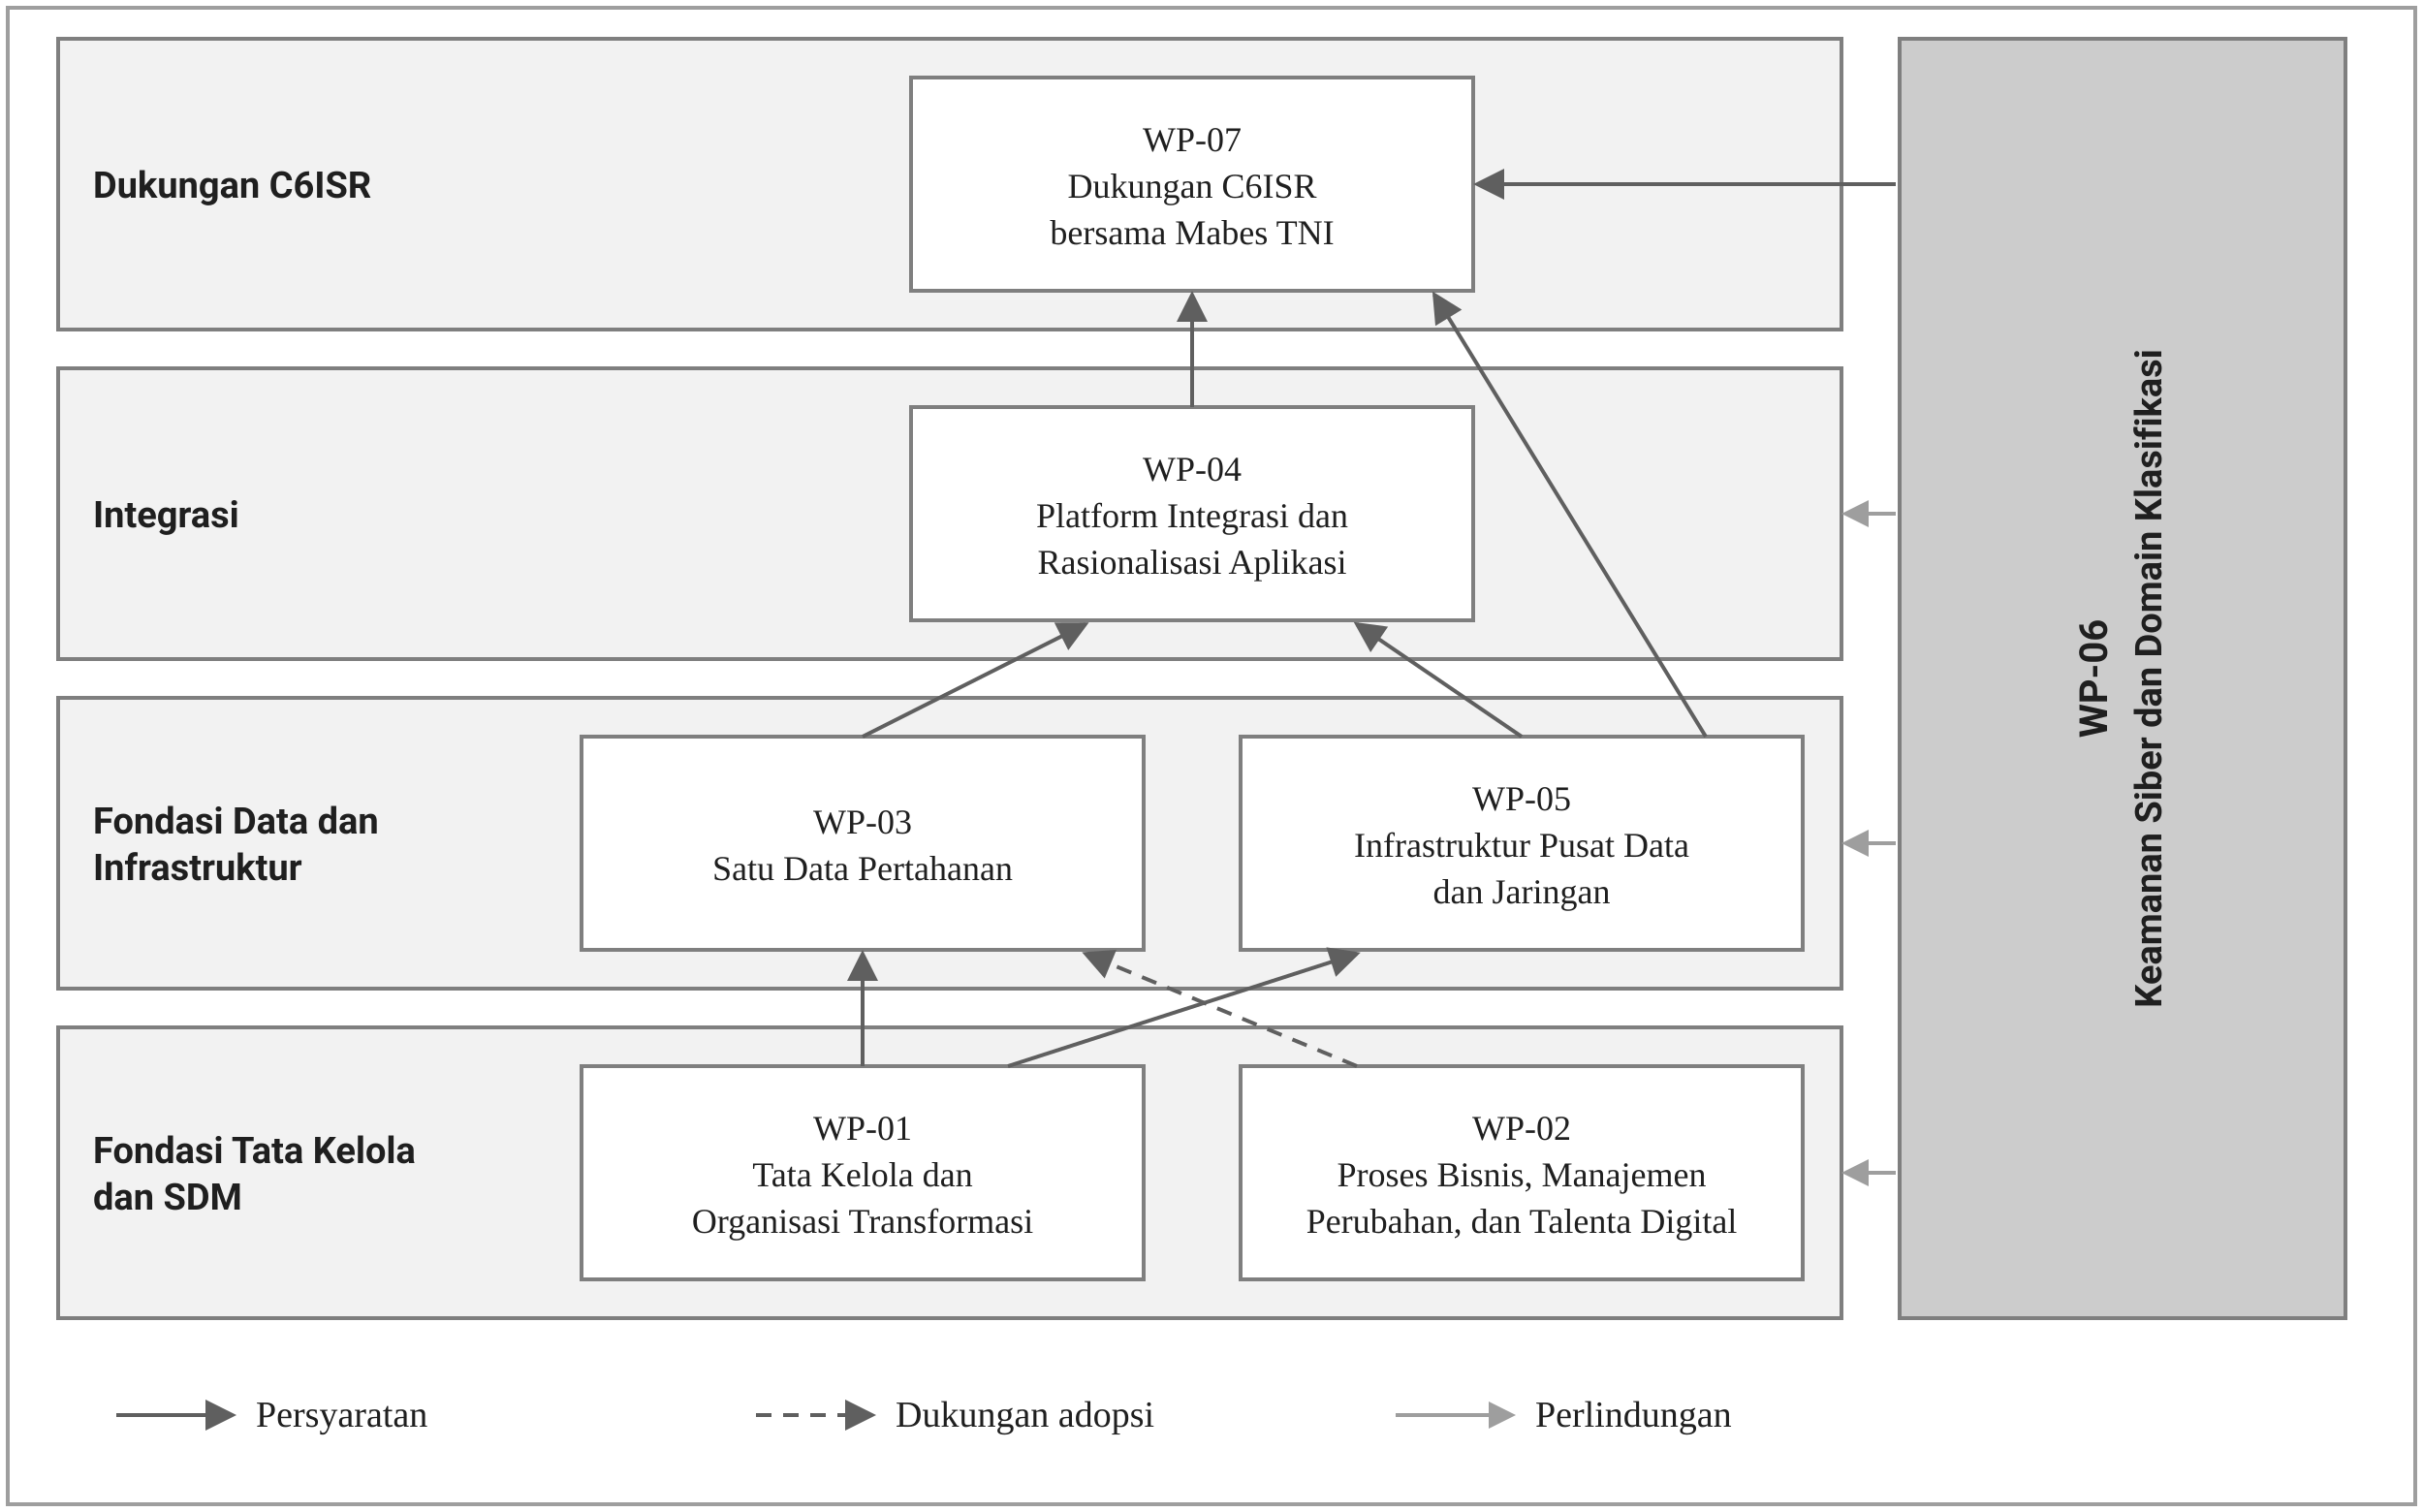
\includegraphics[width=1.00\linewidth,height=0.8\textheight,keepaspectratio]{images/Ketergantungan Paket Pekerjaan.png}
\caption{Ketergantungan Paket Pekerjaan}
\label{fig:IV.14}
\end{figure}

Gambar~\ref{fig:IV.14} menyusun paket pekerjaan dalam empat lapis. WP-01 dan WP-02 menjadi fondasi karena tanpa mandat dan tata kelola, inisiatif teknis berisiko berjalan parsial. WP-03 dan WP-05 menyediakan data terstandar dan infrastruktur bagi WP-04. WP-07 baru dapat diwujudkan setelah data dapat dipertukarkan melalui WP-04, infrastruktur dan PACE tersedia melalui WP-05, serta jaringan terklasifikasi tersedia melalui WP-06. WP-06 digambarkan vertikal karena melindungi seluruh paket sejak jangka pendek.

\subsection{Kesiapan dan Risiko}
\label{sec:IV.7.4}

Kesiapan transformasi dinilai pada enam faktor \cite{TOGAF2022}, yaitu kepemimpinan dan tata kelola (sedang), SDM digital (rendah–sedang), data dan interoperabilitas (rendah), infrastruktur teknologi (sedang), keamanan siber (sedang), serta regulasi dan kebijakan (tinggi). Penilaian ini didasarkan pada Tabel~\ref{tab:II.1} dan permasalahan prioritas Satu Data Pertahanan \cite{Pusdatin2026SatuData}. Kesiapan tersebut dan risiko pada Tabel~\ref{tab:IV.10} dipetakan ke setiap paket, sebagaimana disajikan pada Tabel~\ref{tab:IV.30}.

\begingroup\small\setstretch{1.0}
\begin{longtable}{@{}>{\raggedright\arraybackslash\hspace{0pt}}p{0.103\linewidth}>{\raggedright\arraybackslash\hspace{0pt}}p{0.263\linewidth}>{\raggedright\arraybackslash\hspace{0pt}}p{0.252\linewidth}>{\raggedright\arraybackslash\hspace{0pt}}p{0.290\linewidth}@{}}
\caption{Kesiapan dan Risiko per Paket Pekerjaan}\label{tab:IV.30}\\
\toprule
\textbf{Paket} & \textbf{Kesiapan} & \textbf{Risiko Utama} & \textbf{Mitigasi dalam Rencana}\\
\midrule
\endfirsthead
\multicolumn{4}{@{}l}{\small\itshape \tablename\ \thetable{} (lanjutan)}\\
\toprule
\textbf{Paket} & \textbf{Kesiapan} & \textbf{Risiko Utama} & \textbf{Mitigasi dalam Rencana}\\
\midrule
\endhead
\bottomrule
\endlastfoot
WP-01 & Kepemimpinan dan tata kelola (sedang); regulasi (tinggi) & Resistensi perubahan organisasi & Mandat DTO ditetapkan sejak jangka pendek dengan dukungan pimpinan\\*
WP-02 & SDM digital (rendah–sedang) & Keterbatasan SDM digital & Pelatihan, rekrutmen, dan kerja sama kelembagaan berjalan paralel\\
WP-03 & Data dan interoperabilitas (rendah); regulasi (tinggi) & Kompleksitas integrasi sistem \textit{legacy} & Standar data ditetapkan sebelum portal dibangun\\
WP-04 & Data dan interoperabilitas (rendah) & Kompleksitas integrasi sistem \textit{legacy} & Integrasi bertahap melalui API dan standar terbuka\\
WP-05 & Infrastruktur teknologi (sedang) & Keterbatasan anggaran dan waktu & Investasi infrastruktur ditahapkan berdasarkan prioritas\\
WP-06 & Keamanan siber (sedang) & Ancaman siber selama transisi & Keamanan dasar didahulukan dan \textit{security by design} diterapkan pada setiap paket\\*
WP-07 & Data dan interoperabilitas (rendah) & Penerapan DERA tidak seragam antarorganisasi & Standar pertukaran data ditetapkan bersama Mabes TNI melalui \textit{Architecture Board}\\
\end{longtable}
\endgroup

Tabel~\ref{tab:IV.30} menunjukkan bahwa WP-03, WP-04, dan WP-07 memiliki kesiapan terendah karena bergantung pada data dan interoperabilitas. Oleh karena itu, jangka pendek pada ketiga paket tersebut difokuskan pada penetapan standar yang berbiaya rendah tetapi menurunkan risiko integrasi.

\subsection{Arsitektur Transisi}
\label{sec:IV.7.5}

Berdasarkan ketergantungan dan kesiapan tersebut, strategi implementasi yang dipilih adalah pendekatan bertahap dengan prinsip fondasi terlebih dahulu. Pendekatan ini sejalan dengan tahapan adopsi DERA pada III.5.3 dan menghasilkan dua arsitektur transisi sebelum arsitektur target tercapai, sebagaimana disajikan pada Tabel~\ref{tab:IV.31}.

\begingroup\small\setstretch{1.0}
\begin{longtable}{@{}>{\raggedright\arraybackslash\hspace{0pt}}p{0.149\linewidth}>{\raggedright\arraybackslash\hspace{0pt}}p{0.252\linewidth}>{\raggedright\arraybackslash\hspace{0pt}}p{0.255\linewidth}>{\raggedright\arraybackslash\hspace{0pt}}p{0.252\linewidth}@{}}
\caption{Arsitektur Transisi per Domain}\label{tab:IV.31}\\
\toprule
\textbf{Domain} & \textbf{Transisi Tahap 1 (Fondasi Tata Kelola dan Standar)} & \textbf{Transisi Tahap 2 (Integrasi Data dan Platform)} & \textbf{Arsitektur Target (Pertahanan Cerdas Terintegrasi)}\\
\midrule
\endfirsthead
\multicolumn{4}{@{}l}{\small\itshape \tablename\ \thetable{} (lanjutan)}\\
\toprule
\textbf{Domain} & \textbf{Transisi Tahap 1 (Fondasi Tata Kelola dan Standar)} & \textbf{Transisi Tahap 2 (Integrasi Data dan Platform)} & \textbf{Arsitektur Target (Pertahanan Cerdas Terintegrasi)}\\
\midrule
\endhead
\bottomrule
\endlastfoot
Bisnis & DTO dan \textit{Architecture Board} berjalan; DERA diadopsi & Proses bisnis terstandar; koordinasi lintas matra terlembaga & Budaya transformasi berkelanjutan\\*
Data & Penyelenggara Satu Data, klasifikasi, dan kamus data ditetapkan & Portal Satu Data Pertahanan beroperasi & Interoperabilitas dengan Portal Satu Data Indonesia\\
Aplikasi & Peta rasionalisasi aplikasi tersedia & Platform integrasi dan SSO/IAM beroperasi; aplikasi berfungsi serupa digabungkan & Aplikasi terintegrasi penuh; dasbor eksekutif beroperasi\\
Teknologi & Pusat pemulihan bencana dan keamanan dasar tersedia & Virtualisasi, jaringan tersegmentasi, PACE, pusat operasi keamanan, dan jaringan terklasifikasi beroperasi & Pusat data aktif-aktif; kematangan keamanan siber level 3\\*
C6ISR & Standar pertukaran data situasi dan hak akses TPT ditetapkan & TPT tingkat strategis dikembangkan & TPT beroperasi bersama Mabes TNI\\
\end{longtable}
\endgroup

Tabel~\ref{tab:IV.31} menunjukkan bahwa keluaran Tahap 1 sebagian besar berupa keputusan, regulasi, dan standar. Tahap 2 menghasilkan integrasi data dan platform, sedangkan arsitektur target mewujudkan keterpaduan pada seluruh domain, termasuk dukungan C6ISR bersama Mabes TNI.

\subsection{Roadmap Arsitektur}
\label{sec:IV.7.6}

Paket pekerjaan, ketergantungan, dan arsitektur transisi dirangkum menjadi \textit{roadmap} arsitektur, sebagaimana ditunjukkan pada Gambar~\ref{fig:IV.15}.

\begin{figure}[htbp]
\centering
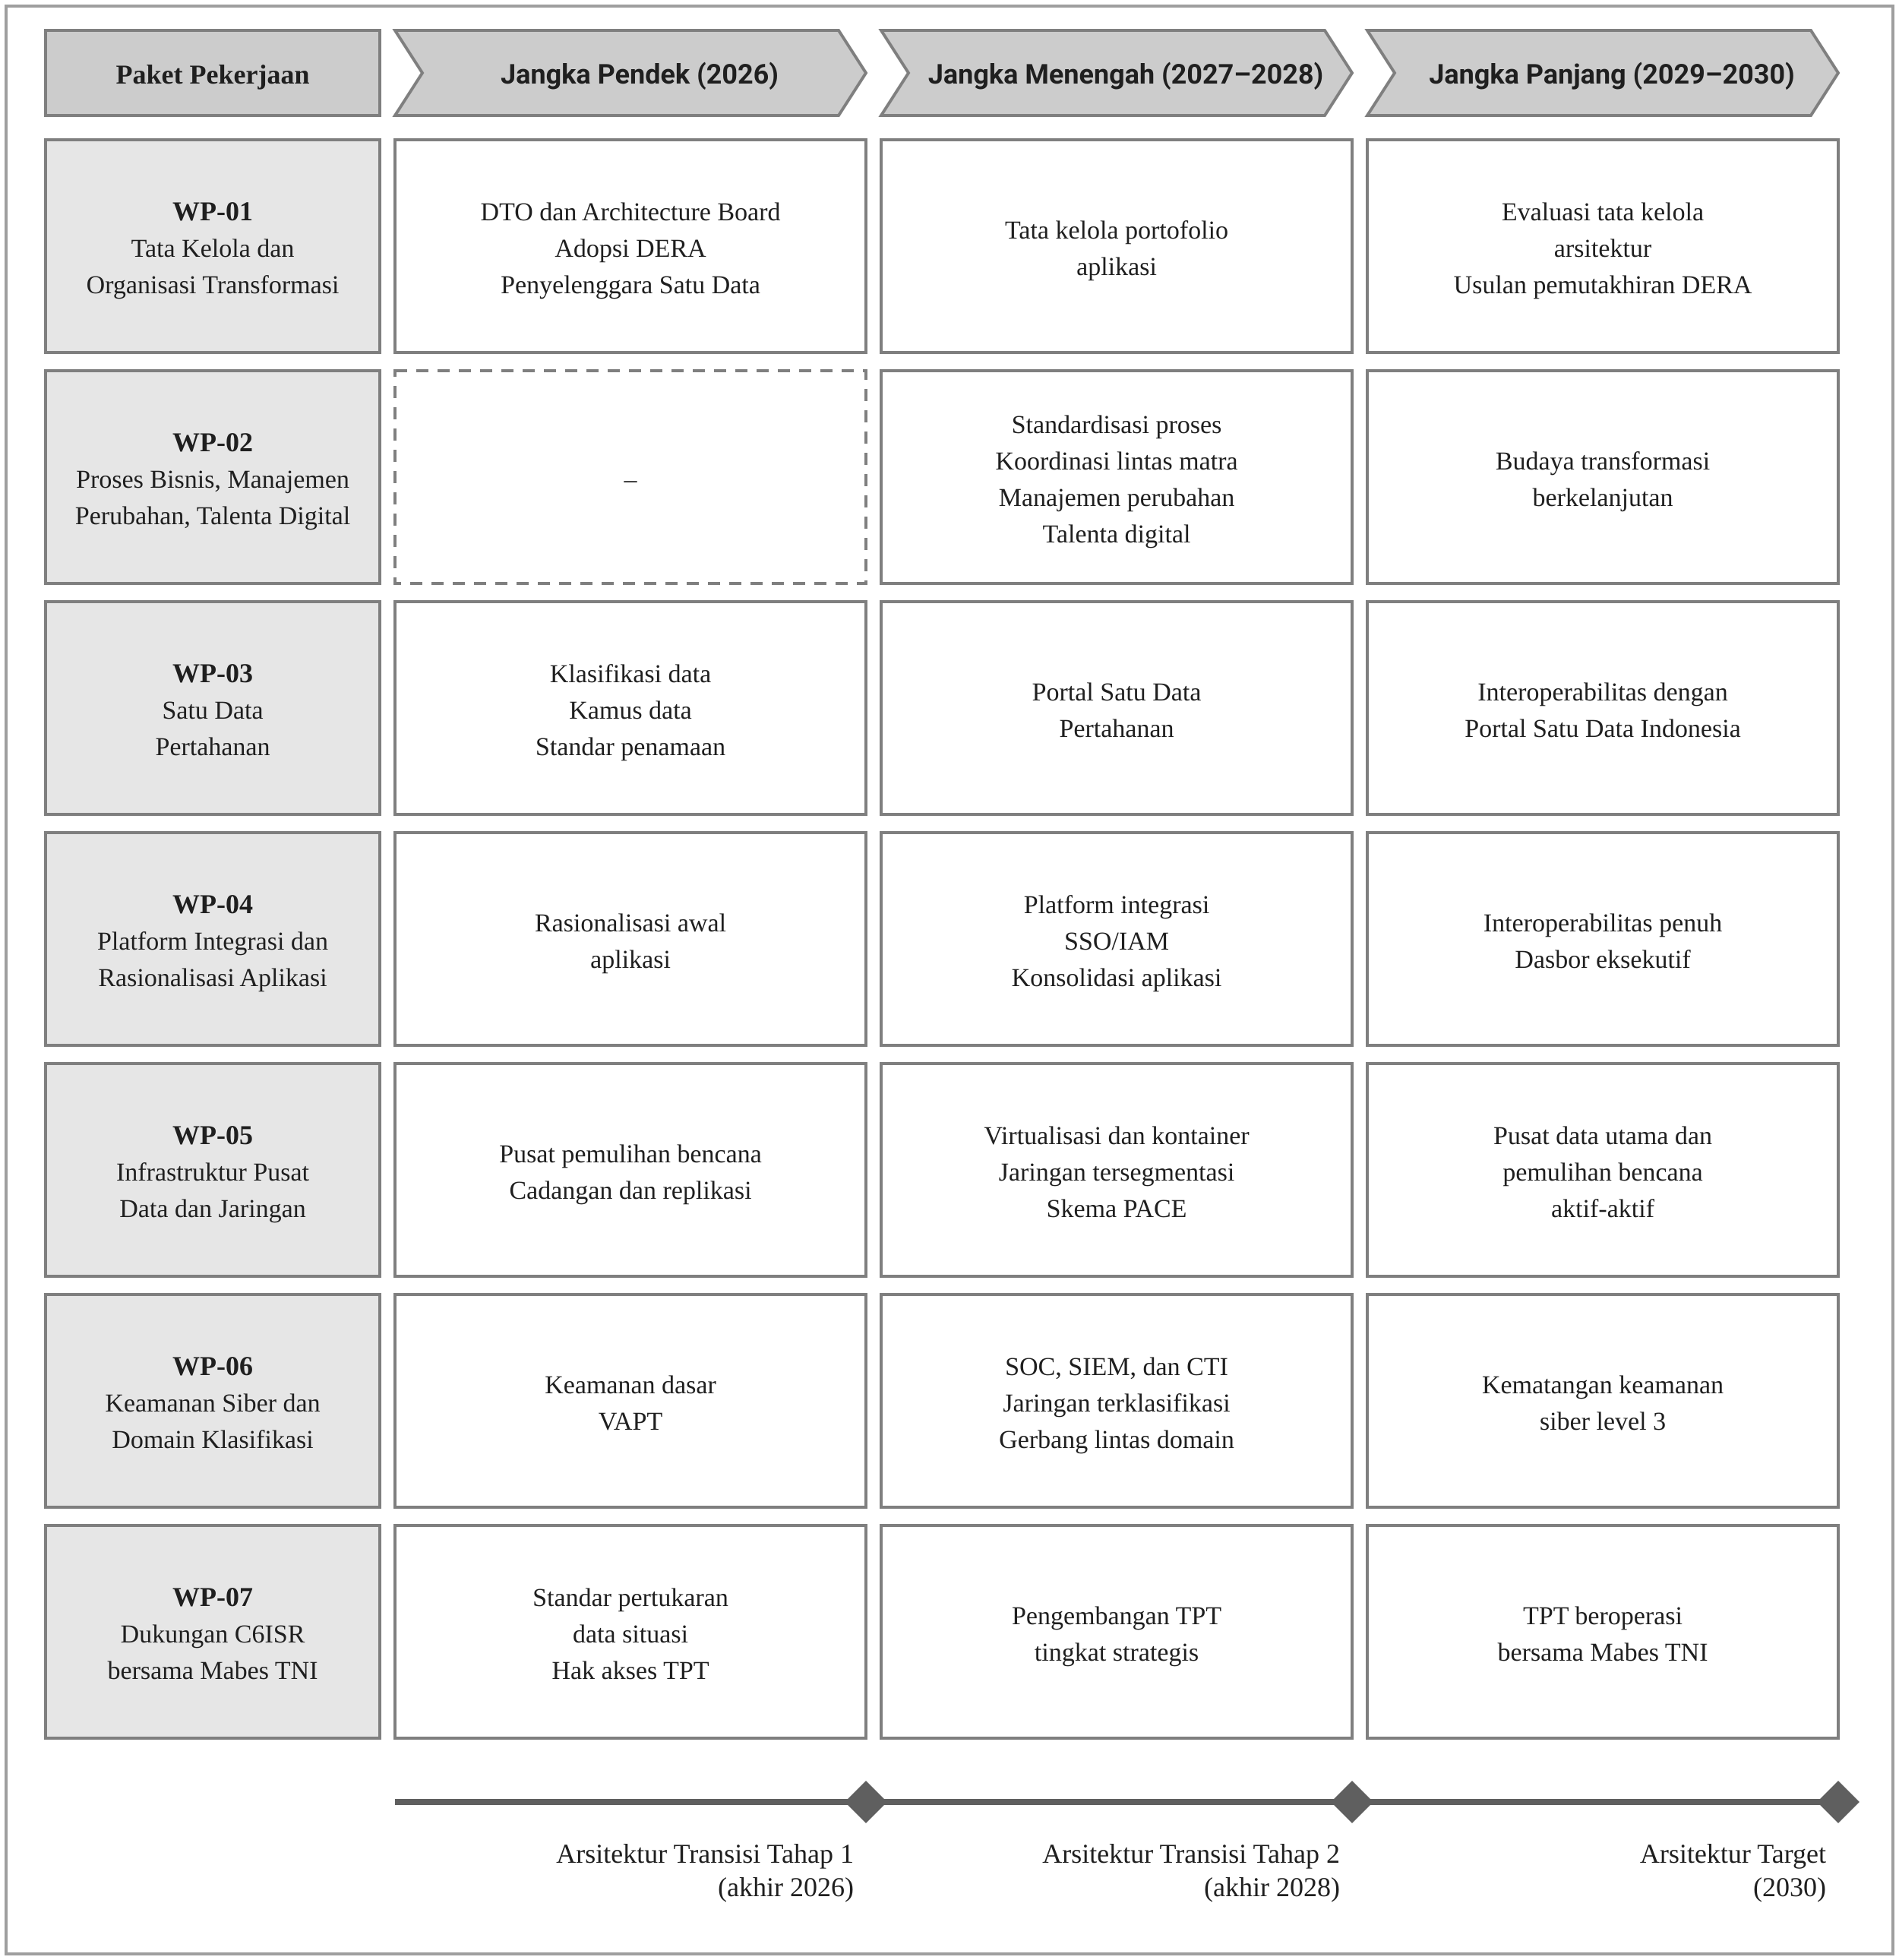
\includegraphics[width=0.96\linewidth,height=0.8\textheight,keepaspectratio]{images/Roadmap Arsitektur.png}
\caption{\textit{Roadmap} Arsitektur}
\label{fig:IV.15}
\end{figure}

Gambar~\ref{fig:IV.15} menempatkan setiap paket pekerjaan pada tiga horizon waktu, yaitu jangka pendek (2026), jangka menengah (2027–2028), dan jangka panjang (2029–2030). Penanda di bagian bawah menunjukkan saat tercapainya Arsitektur Transisi Tahap 1, Arsitektur Transisi Tahap 2, dan Arsitektur Target. WP-02 baru dimulai pada jangka menengah karena bergantung pada terbentuknya DTO, sedangkan WP-06 berjalan pada seluruh horizon sebagai pelindung paket lainnya.

\section{Fase F: Migration Planning}
\label{sec:IV.8}

Fase \textit{Migration Planning} menyusun rencana implementasi dan migrasi berdasarkan paket pekerjaan, arsitektur transisi, dan \textit{roadmap} arsitektur. Fase ini menggunakan CRM dan tahapan adopsi DERA sebagai acuan prioritas (Tabel~\ref{tab:III.22}).

\subsection{Tata Kelola Implementasi}
\label{sec:IV.8.1}

Rencana implementasi dihubungkan dengan tata kelola arsitektur, perencanaan dan penganggaran, serta pengawasan, sebagaimana disajikan pada Tabel~\ref{tab:IV.32}.

\begingroup\small\setstretch{1.0}
\begin{longtable}{@{}>{\raggedright\arraybackslash\hspace{0pt}}p{0.201\linewidth}>{\raggedright\arraybackslash\hspace{0pt}}p{0.307\linewidth}>{\raggedright\arraybackslash\hspace{0pt}}p{0.430\linewidth}@{}}
\caption{Model Tata Kelola Implementasi}\label{tab:IV.32}\\
\toprule
\textbf{Peran} & \textbf{Pihak} & \textbf{Tanggung Jawab}\\
\midrule
\endfirsthead
\multicolumn{3}{@{}l}{\small\itshape \tablename\ \thetable{} (lanjutan)}\\
\toprule
\textbf{Peran} & \textbf{Pihak} & \textbf{Tanggung Jawab}\\
\midrule
\endhead
\bottomrule
\endlastfoot
Pengarah & Menteri Pertahanan; Sekretaris Jenderal & Menetapkan arah kebijakan serta menyetujui prioritas dan anggaran transformasi\\*
Pengendali arsitektur & DTO dan \textit{Architecture Board} & Menetapkan kontrak arsitektur dan menilai kesesuaian proyek berdasarkan KK-01 hingga KK-09\\
Pengelola program & DTO (Bidang Strategi dan \textit{Roadmap} Transformasi Digital) & Mengoordinasikan jadwal, ketergantungan, dan pelaporan kemajuan paket pekerjaan\\
Perencana dan penganggar & Ditjen Perencanaan Pertahanan; Biro Perencanaan dan Keuangan & Menyelaraskan paket pekerjaan dengan dokumen perencanaan dan penganggaran pertahanan\\
Pelaksana & Pusat Data dan Informasi; Pusat Siber dan Intelijen Teknologi Pertahanan; satuan kerja terkait & Melaksanakan paket pekerjaan sesuai kontrak arsitektur\\
Mitra operasional & Mabes TNI dan ketiga matra & Melaksanakan dan memvalidasi WP-07 bersama Kemhan RI\\*
Pengawas & Inspektorat Jenderal & Mengawasi kepatuhan pelaksanaan terhadap peraturan perundang-undangan\\
\end{longtable}
\endgroup

Tabel~\ref{tab:IV.32} menunjukkan bahwa setiap proyek dilaksanakan berdasarkan kontrak arsitektur antara \textit{Architecture Board} dan pelaksana. Kontrak tersebut memuat lingkup proyek, standar yang wajib dipenuhi, dan kriteria penerimaan, termasuk kriteria kesesuaian DERA.

\subsection{Nilai Manfaat dan Sumber Daya}
\label{sec:IV.8.2}

Nilai manfaat setiap paket ditentukan dari kontribusinya terhadap tujuan strategis pada Tabel~\ref{tab:IV.7}. Karena data anggaran rinci belum tersedia, kebutuhan biaya dikelompokkan ke dalam tiga kelas, yaitu rendah untuk penetapan regulasi dan penataan organisasi, sedang untuk pengembangan sistem, serta tinggi untuk pembangunan infrastruktur fisik. Hasilnya disajikan pada Tabel~\ref{tab:IV.33}.

\begingroup\small\setstretch{1.0}
\begin{longtable}{@{}>{\raggedright\arraybackslash\hspace{0pt}}p{0.103\linewidth}>{\raggedright\arraybackslash\hspace{0pt}}p{0.194\linewidth}>{\raggedright\arraybackslash\hspace{0pt}}p{0.450\linewidth}>{\raggedright\arraybackslash\hspace{0pt}}p{0.160\linewidth}@{}}
\caption{Nilai Manfaat dan Kebutuhan Sumber Daya Paket Pekerjaan}\label{tab:IV.33}\\
\toprule
\textbf{Paket} & \textbf{Tujuan Strategis} & \textbf{Sarana Penyampaian} & \textbf{Kelas Biaya}\\
\midrule
\endfirsthead
\multicolumn{4}{@{}l}{\small\itshape \tablename\ \thetable{} (lanjutan)}\\
\toprule
\textbf{Paket} & \textbf{Tujuan Strategis} & \textbf{Sarana Penyampaian} & \textbf{Kelas Biaya}\\
\midrule
\endhead
\bottomrule
\endlastfoot
WP-01 & 3, 7 & Penetapan regulasi dan penataan organisasi & Rendah\\*
WP-02 & 1, 6 & Standardisasi proses, pelatihan, dan rekrutmen & Sedang\\
WP-03 & 1, 3, 7 & Penetapan regulasi data dan pengembangan sistem & Sedang\\
WP-04 & 1, 3, 6 & Pengembangan sistem dan penggabungan aplikasi & Sedang\\
WP-05 & 1, 4, 5 & Pembangunan pusat pemulihan bencana, jaringan, dan sarana komunikasi & Tinggi\\
WP-06 & 2, 4 & Pengadaan perangkat keamanan dan pembentukan pusat operasi keamanan & Sedang\\*
WP-07 & 1, 3, 4 & Penetapan standar dan pengembangan TPT bersama Mabes TNI & Sedang\\
\end{longtable}
\endgroup

Tabel~\ref{tab:IV.33} menunjukkan bahwa WP-03, WP-04, WP-05, dan WP-07 mendukung tiga tujuan strategis sekaligus. Namun, WP-05 membutuhkan biaya tertinggi karena melibatkan infrastruktur fisik.

\subsection{Prioritas Paket Pekerjaan}
\label{sec:IV.8.3}

Prioritas paket pekerjaan ditentukan berdasarkan empat kriteria dengan skor 1–3, yaitu:

\begin{enumerate}[label=\arabic*.]
\item manfaat strategis, berdasarkan jumlah tujuan strategis pada Tabel~\ref{tab:IV.33} (satu tujuan = 1, dua tujuan = 2, tiga tujuan = 3);
\item biaya, berdasarkan kelas biaya pada Tabel~\ref{tab:IV.33} (tinggi = 1, sedang = 2, rendah = 3);
\item kesiapan, berdasarkan tingkat kesiapan terendah pada Tabel~\ref{tab:IV.30} (rendah atau rendah–sedang = 1, sedang = 2, tinggi = 3); dan
\item ketergantungan, berdasarkan jumlah paket yang mensyaratkan paket tersebut pada Gambar~\ref{fig:IV.14} (tidak ada = 1, satu paket = 2, dua paket atau lebih = 3).
\end{enumerate}

Skor keempat kriteria dijumlahkan dengan rentang 4–12. Paket dengan skor 9–12 ditetapkan sebagai Prioritas I, skor 7–8 sebagai Prioritas II, dan skor 4–6 sebagai Prioritas III. Hasilnya disajikan pada Tabel~\ref{tab:IV.34}.

\begingroup\small\setstretch{1.0}
\begin{longtable}{@{}>{\raggedright\arraybackslash\hspace{0pt}}p{0.097\linewidth}>{\raggedright\arraybackslash\hspace{0pt}}p{0.108\linewidth}>{\raggedright\arraybackslash\hspace{0pt}}p{0.087\linewidth}>{\raggedright\arraybackslash\hspace{0pt}}p{0.118\linewidth}>{\raggedright\arraybackslash\hspace{0pt}}p{0.183\linewidth}>{\raggedright\arraybackslash\hspace{0pt}}p{0.087\linewidth}>{\raggedright\arraybackslash\hspace{0pt}}p{0.133\linewidth}@{}}
\caption{Skor Prioritas Paket Pekerjaan}\label{tab:IV.34}\\
\toprule
\textbf{Paket} & \textbf{Manfaat} & \textbf{Biaya} & \textbf{Kesiapan} & \textbf{Ketergantungan} & \textbf{Total} & \textbf{Prioritas}\\
\midrule
\endfirsthead
\multicolumn{7}{@{}l}{\small\itshape \tablename\ \thetable{} (lanjutan)}\\
\toprule
\textbf{Paket} & \textbf{Manfaat} & \textbf{Biaya} & \textbf{Kesiapan} & \textbf{Ketergantungan} & \textbf{Total} & \textbf{Prioritas}\\
\midrule
\endhead
\bottomrule
\endlastfoot
WP-01 & \centering\arraybackslash 2 & \centering\arraybackslash 3 & \centering\arraybackslash 2 & \centering\arraybackslash 3 & \centering\arraybackslash 10 & \centering\arraybackslash I\\*
WP-05 & \centering\arraybackslash 3 & \centering\arraybackslash 1 & \centering\arraybackslash 2 & \centering\arraybackslash 3 & \centering\arraybackslash 9 & \centering\arraybackslash I\\
WP-06 & \centering\arraybackslash 2 & \centering\arraybackslash 2 & \centering\arraybackslash 2 & \centering\arraybackslash 3 & \centering\arraybackslash 9 & \centering\arraybackslash I\\
WP-03 & \centering\arraybackslash 3 & \centering\arraybackslash 2 & \centering\arraybackslash 1 & \centering\arraybackslash 2 & \centering\arraybackslash 8 & \centering\arraybackslash II\\
WP-04 & \centering\arraybackslash 3 & \centering\arraybackslash 2 & \centering\arraybackslash 1 & \centering\arraybackslash 2 & \centering\arraybackslash 8 & \centering\arraybackslash II\\
WP-07 & \centering\arraybackslash 3 & \centering\arraybackslash 2 & \centering\arraybackslash 1 & \centering\arraybackslash 1 & \centering\arraybackslash 7 & \centering\arraybackslash II\\*
WP-02 & \centering\arraybackslash 2 & \centering\arraybackslash 2 & \centering\arraybackslash 1 & \centering\arraybackslash 1 & \centering\arraybackslash 6 & \centering\arraybackslash III\\
\end{longtable}
\endgroup

Tabel~\ref{tab:IV.34} menunjukkan bahwa Prioritas I terdiri atas WP-01, WP-05, dan WP-06. Ketiganya menjadi prasyarat atau pelindung paket lainnya, dan WP-05 menutup risiko terbesar, yaitu titik tunggal kegagalan pusat data. Skor ketergantungan WP-06 dihitung dari perannya melindungi seluruh paket. Prioritas menunjukkan urutan pemusatan sumber daya, bukan tingkat kepentingan. WP-07 memiliki manfaat strategis tinggi, tetapi berada pada Prioritas II karena kesiapannya rendah dan bergantung pada tiga paket lainnya.

\subsection{Rencana Implementasi dan Migrasi 2026–2030}
\label{sec:IV.8.4}

Berdasarkan prioritas tersebut, implementasi dilaksanakan dalam tiga tahap migrasi. Setiap tahap diakhiri dengan tinjauan \textit{Architecture Board} sebelum tahap berikutnya dimulai, sebagaimana disajikan pada Tabel~\ref{tab:IV.35}.

\begingroup\small\setstretch{1.0}
\begin{longtable}{@{}>{\raggedright\arraybackslash\hspace{0pt}}p{0.217\linewidth}>{\raggedright\arraybackslash\hspace{0pt}}p{0.149\linewidth}>{\raggedright\arraybackslash\hspace{0pt}}p{0.301\linewidth}>{\raggedright\arraybackslash\hspace{0pt}}p{0.240\linewidth}@{}}
\caption{Tahapan Migrasi 2026–2030}\label{tab:IV.35}\\
\toprule
\textbf{Tahap} & \textbf{Periode} & \textbf{Fokus Paket Pekerjaan} & \textbf{Titik Keputusan}\\
\midrule
\endfirsthead
\multicolumn{4}{@{}l}{\small\itshape \tablename\ \thetable{} (lanjutan)}\\
\toprule
\textbf{Tahap} & \textbf{Periode} & \textbf{Fokus Paket Pekerjaan} & \textbf{Titik Keputusan}\\
\midrule
\endhead
\bottomrule
\endlastfoot
Tahap 1: Fondasi Tata Kelola dan Standar & 2026 & WP-01, WP-05, dan WP-06 (Prioritas I); inisiatif jangka pendek WP-03, WP-04, dan WP-07 & Tinjauan Arsitektur Transisi Tahap 1\\*
Tahap 2: Integrasi Data dan Platform & 2027–2028 & WP-03 dan WP-04 (Prioritas II); WP-07 mulai dikembangkan; WP-02 dimulai & Tinjauan Arsitektur Transisi Tahap 2\\*
Tahap 3: Pertahanan Cerdas Terintegrasi & 2029–2030 & Penyelesaian WP-07 dan WP-02 (Prioritas III) serta seluruh paket & Tinjauan arsitektur target dan \textit{Request for Architecture Work} siklus berikutnya\\
\end{longtable}
\endgroup

Tabel~\ref{tab:IV.35} menunjukkan bahwa setiap tahap memiliki titik keputusan. Apabila suatu tahap belum tercapai, \textit{Architecture Board} dapat menyesuaikan jadwal tahap berikutnya tanpa mengubah arsitektur target. Target kematangan keamanan siber level 3 pada tahun 2029 berada pada Tahap 3. Pengalaman penerapan pada setiap tahap juga menjadi umpan balik bagi pemutakhiran DERA.
